\documentclass[9pt]{beamer}
% \documentclass[reqno]{beamer}

\usepackage{booktabs} % better tables

\usepackage{subfigure}

\usepackage{times}
\usepackage[utf8]{inputenc}  % pour les accents
\usepackage{euler}
\usepackage{amsmath}
\usepackage{amssymb}
\usepackage{dsfont}
\usepackage{amsthm}
\usepackage{color}
\usepackage{listings}
\usepackage{algorithm}
\usepackage{algorithmic}
\usepackage{booktabs}       % professional-quality tables
\usepackage{tikz}
\usetikzlibrary{decorations.pathreplacing}

%\newtheorem{algorithm}{Algorithm}

\newcommand\independent{\protect\mathpalette{\protect\independenT}{\perp}}
\def\independenT#1#2{\mathrel{\rlap{$#1#2$}\mkern2mu{#1#2}}} 

\newcommand{\ie}{\emph{i.e.}{}}
\newcommand{\st}{\text{\emph{s.t.}}{}}
\newcommand{\eg}{\emph{e.g.}{}}
\newcommand\iid{\ensuremath{\mathit{i.i.d.}}\ }
\newcommand{\rv}{\emph{r.v.}{}}
\newcommand{\ud}{\text{d}{}}
\newcommand{\ind}{\mathds{1}{}}

\newcommand\red{\color{red} }
\newcommand\blue{\color{blue} }
\newcommand\green{\color{green} }
\newcommand{\crit}{\mathcal{C}}

\definecolor{blue}{rgb}{0.05,0.05,0.8}
\definecolor{red}{rgb}{0.7,0.1,0.1}
\definecolor{green}{rgb}{0.1,0.4,0.1}

\def\argmin{\operatornamewithlimits{arg\,min}}
\def\argmax{\operatornamewithlimits{arg\,max}}
\def\supess{\operatornamewithlimits{ess\,sup}}

% \DeclareMathOperator{\argmin}{argmin}
\def\bb{\mathbb}
\def\mb{\mathbf}
\def\leb{\text{Leb}}


% \usetheme{Darmstadt} %\theme
% \useoutertheme{sidebar}
% \useinnertheme{circles}

%\usecolortheme{beaver}
%\usecolortheme{seagull}
\usecolortheme{seahorse}
%\setbeamercolor*{frametitle}{parent=palette primary}


% \useoutertheme{infolines}
\setbeamertemplate{navigation symbols}{} 
\setbeamertemplate{footline}{
  \hspace*{.5cm}\tiny{%\insertauthor
    \hspace*{50pt}
    \hfill\insertframenumber%/\inserttotalframenumber
    \hspace*{.5cm}}\vspace*{.1cm}} 

% \addtobeamertemplate{footline}{\insertframenumber}%/\inserttotalframenumber} 
% \setbeamertemplate{footline}{\hspace*{.5cm}\scriptsize{%\insertauthor
%     \hspace*{50pt} \hfill\insertframenumber\hspace*{.5cm}}\vspace*{.1cm}} 

%\setbeamertemplate{theorems}[numbered]

 \setbeamercolor{block title}{bg=blue!10,fg=blue}
 \setbeamercolor{block body}{bg=blue!10,fg=black}

% %\setbeamercolor{block title alerted}{bg=green!10,fg=black}
% \setbeamercolor{block body alerted}{bg=red!10,fg=black}

 \setbeamercolor{block title example}{bg=green!10,fg=green}
 \setbeamercolor{block body example}{bg=green!10,fg=black}


\title{
Machine Learning and Extremes  for Anomaly Detection
}

\author[Nicolas Goix]{ Nicolas Goix \\
% \\
% \vspace{1em}
 {\footnotesize LTCI, CNRS, Telecom ParisTech, Université Paris-Saclay, France 
 }
}
%}
\date{PhD Defense, Telecom Paristech, November 28th 2016}



\AtBeginSection[]
{
 \begin{frame}<beamer>
 \frametitle{}
 \tableofcontents[currentsection]
 \end{frame}
}

\begin{document}
\begin{frame}
 \titlepage
\end{frame}


% \begin{frame}
% \frametitle{Outline}
% \tableofcontents%[section, subsection]
% \end{frame}

% \begin{frame}
%   \frametitle{Outline}
%   \tableofcontents
% \end{frame}


%\section{Introduction}


\begin{frame}
\frametitle{Anomaly Detection (AD)}

\textbf{`Finding patterns in the data that do not conform to expected behavior'}
\begin{figure}
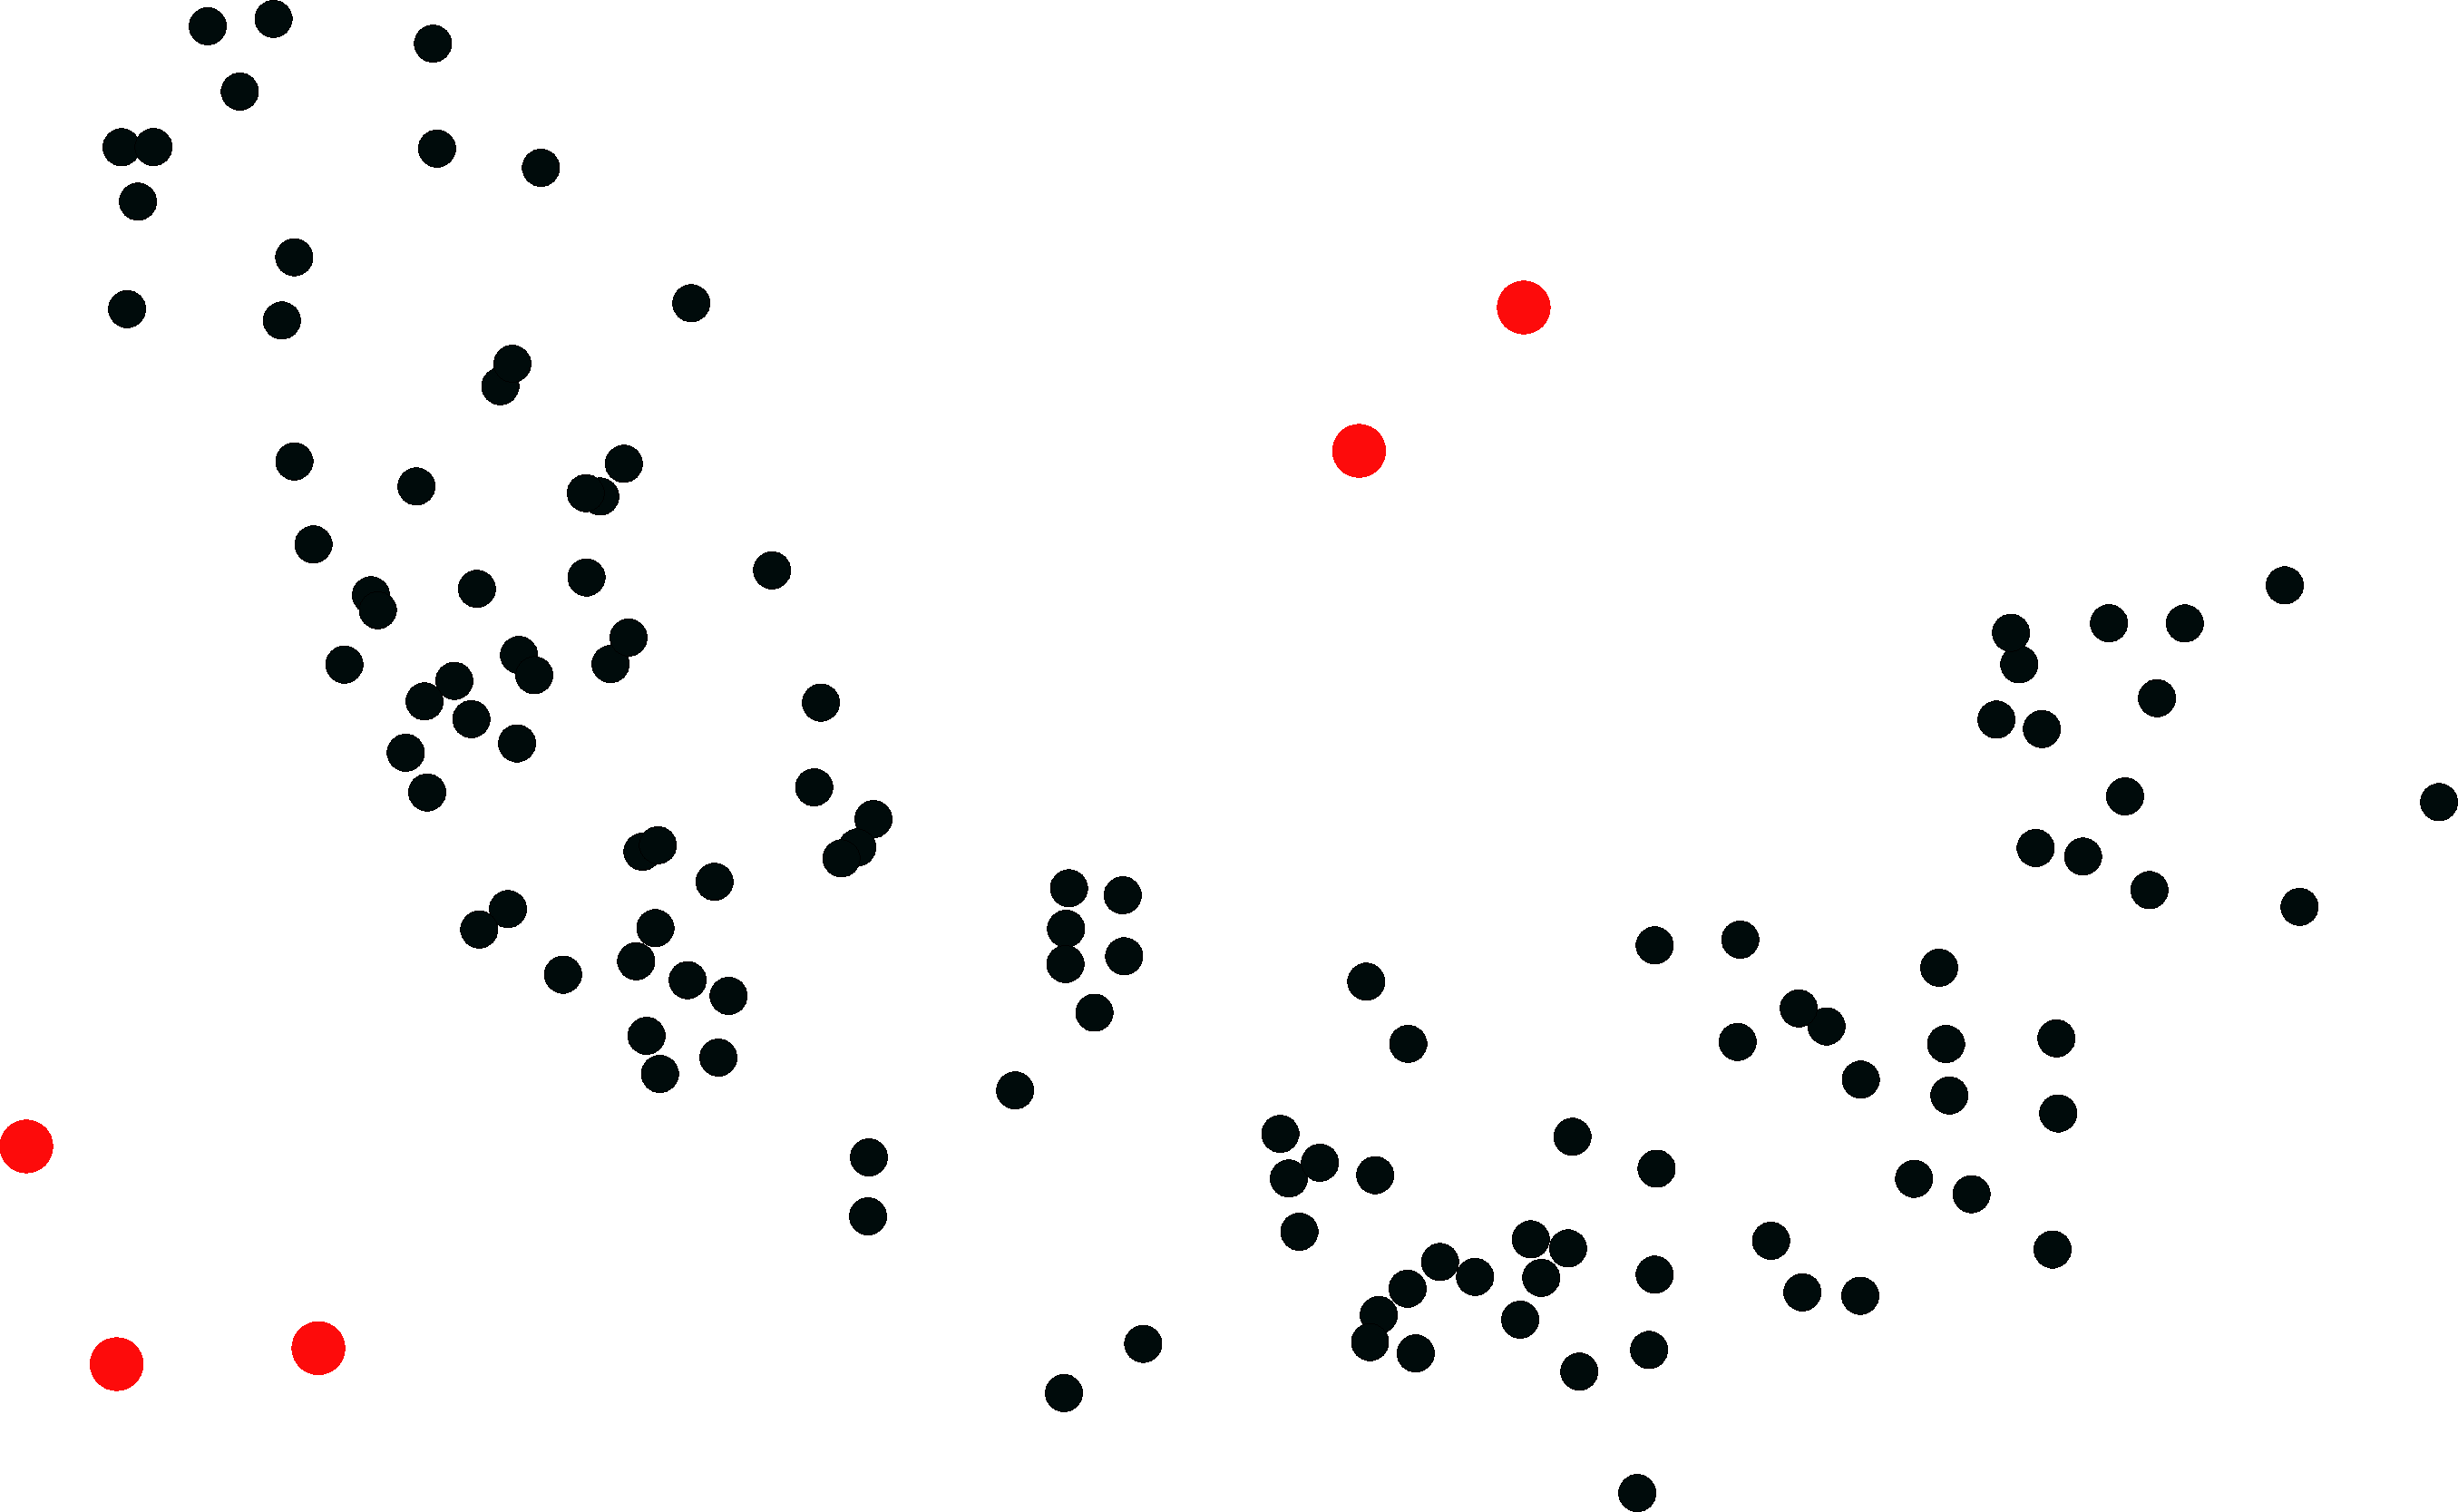
\includegraphics[height=4cm]{sourcefigs/AD_intro.pdf}
\end{figure}
\textbf{Applications}: Network intrusions, credit card fraud detection, insurance, finance, military surveillance, predictive maintenance... \\~\\
\end{frame}



\begin{frame}
\frametitle{Machine Learning context}
%In a machine learning context, AD can been seen as a classification task but where the usual assumption -dataset contains info regarding all classes- breaks down.
\begin{block}{Different kinds of Anomaly Detection}
\begin{itemize}
\item \textbf{Supervised} AD {\red (not dealt with)}\\
Labels available for both normal data and anomalies\\
(similar to rare class mining)\\~\\

\item \textbf{Novelty Detection} {\red (our theoretical framework)}\\
Synonym: one-class classification.
The algorithm learns on normal data only\\~\\

\item \textbf{Outlier Detection} {\red (extended application framework)}\\
Training set (unlabeled) = normal + abnormal data \\
(assumption: anomalies are very rare)
\end{itemize}
\end{block}
\begin{figure}
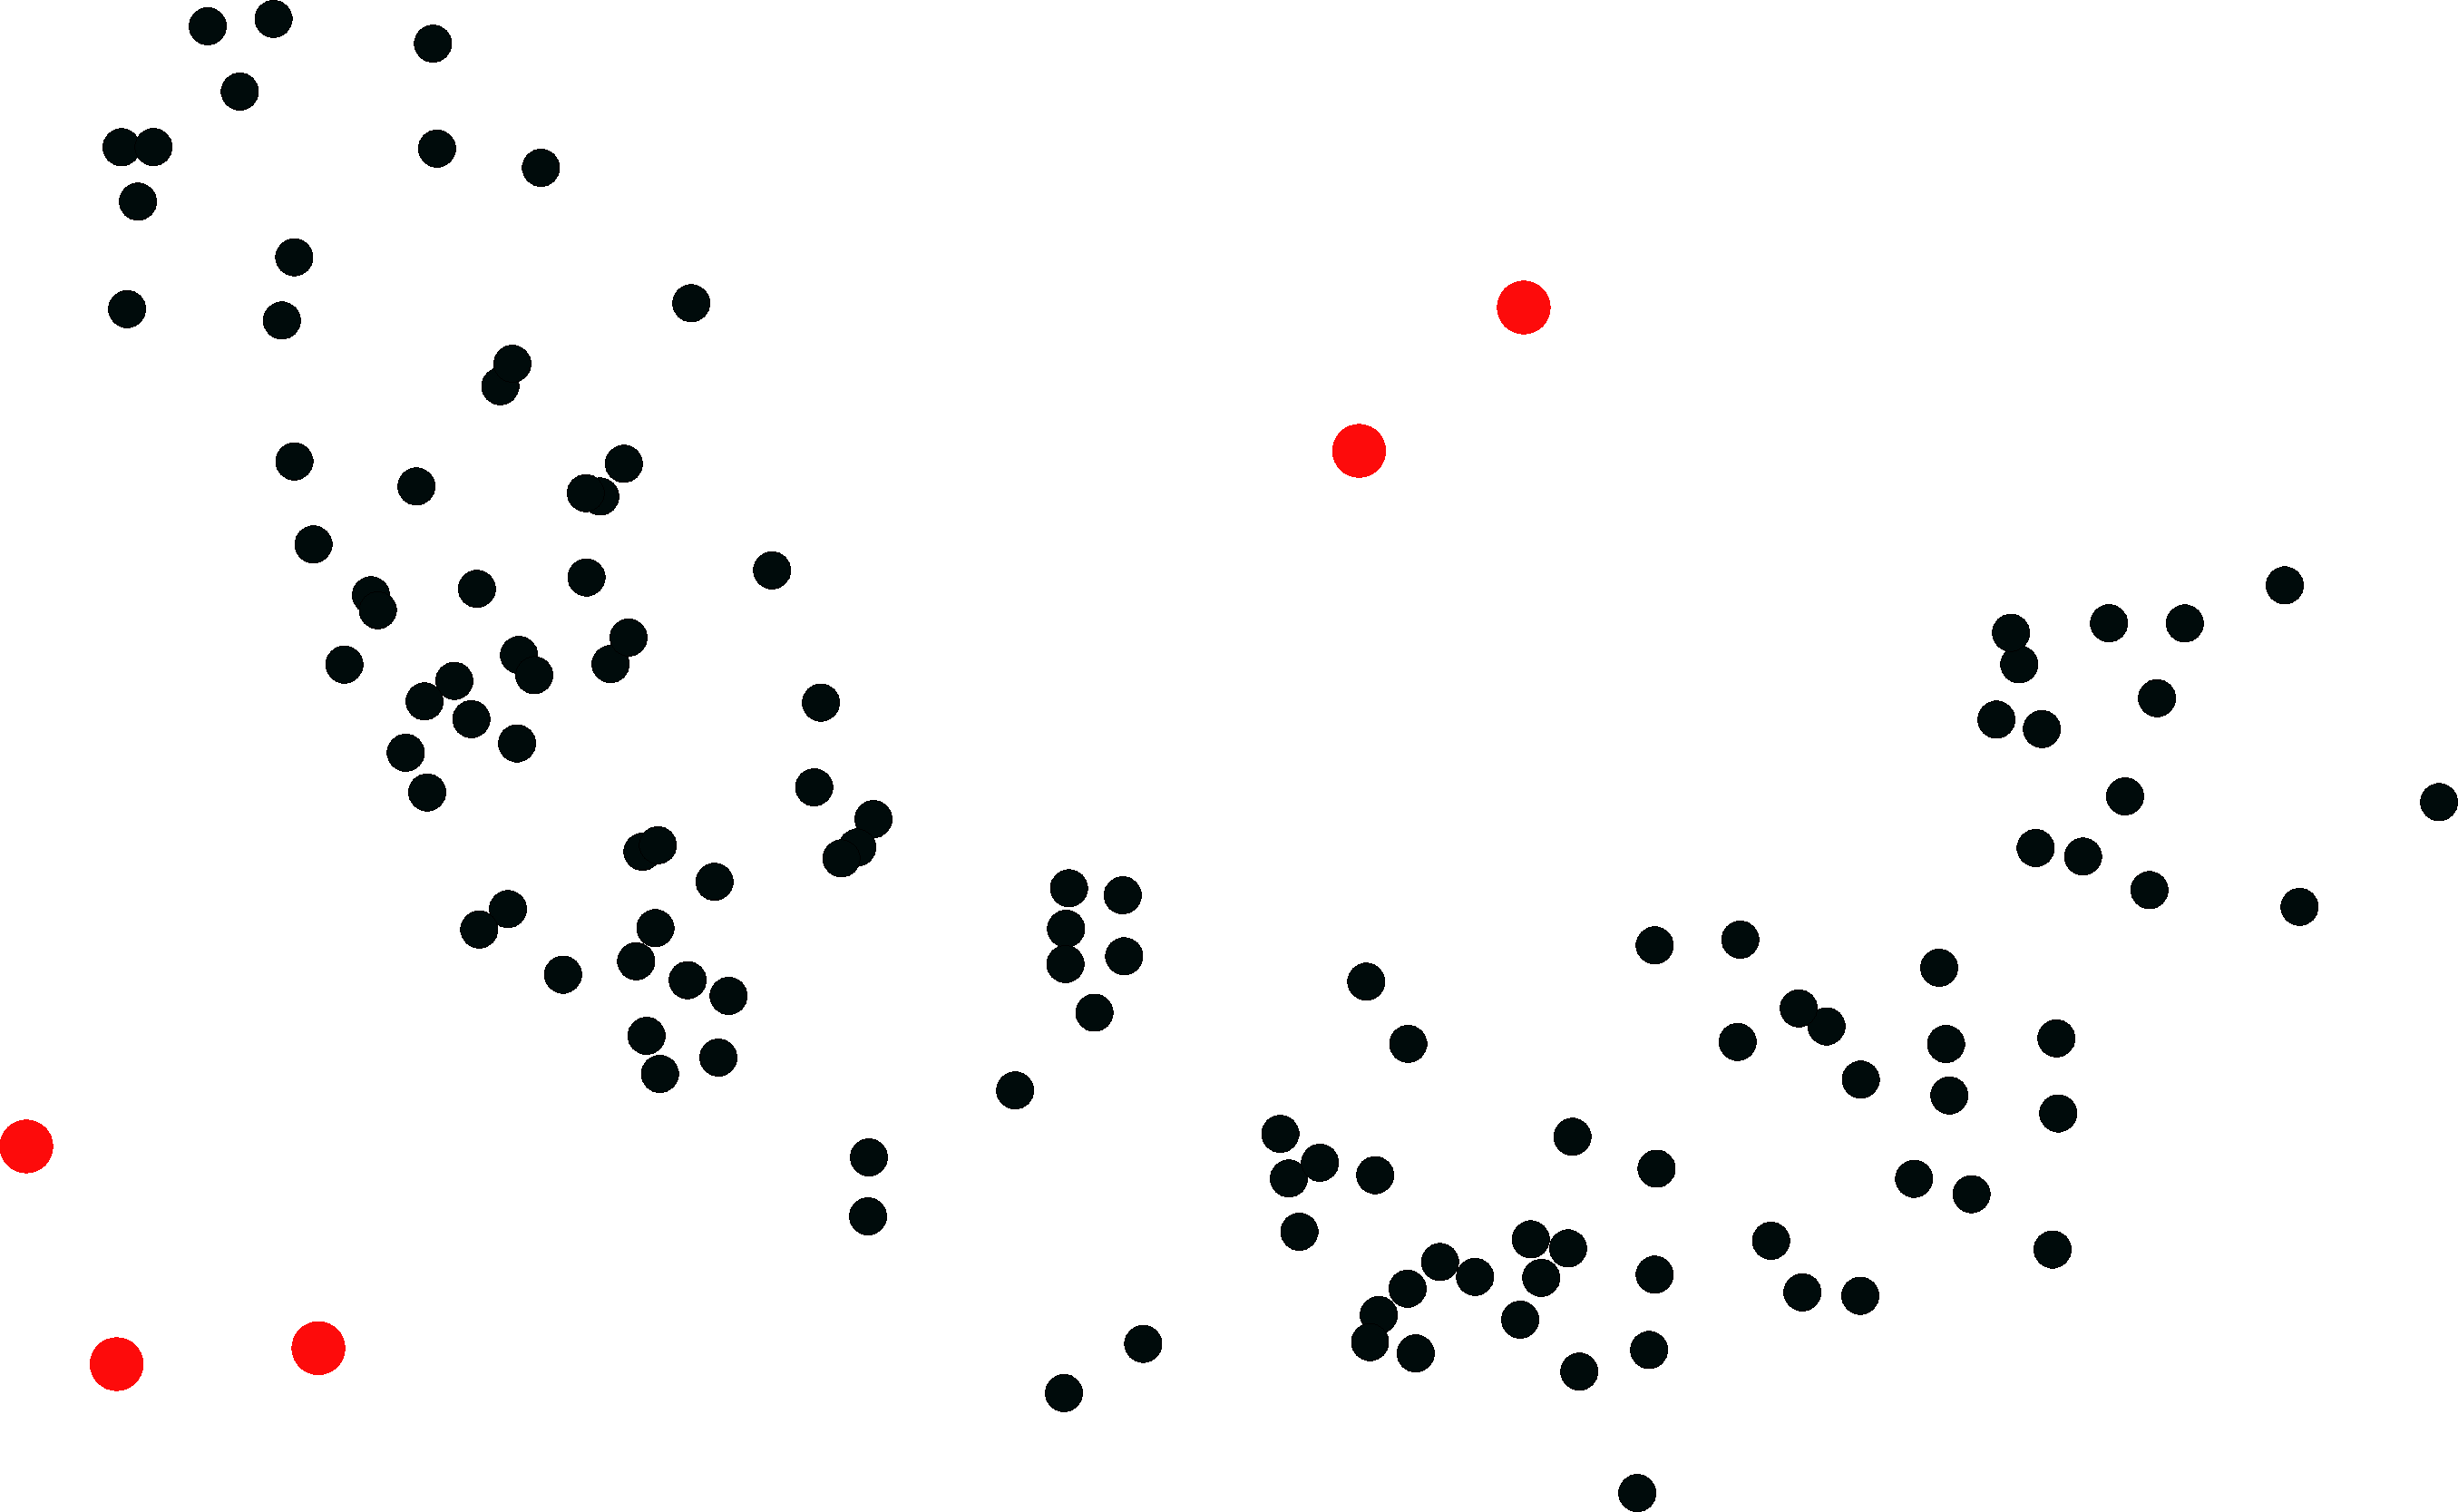
\includegraphics[height=2.7cm]{sourcefigs/AD_intro.pdf}
\end{figure}
\end{frame}


\begin{frame}
\frametitle{Some literature in Anomaly Detection}
%\begin{exampleblock}{Some litterature in Anomaly Detection:}
\begin{itemize}
\item \textbf{Statistical AD techniques}\\
{\small [Hawkins 1980, Liu and Weng 1991, Eskin 2000, Agarwal 2006]}\\~\\

% fit a statistical model for normal behavior (ex: gaussian, gaussian mixture) \\~\\

\item \textbf{K-nearest neighbors}\\
{\small [Breunig \emph{et al.} 2000, Tang \emph{et al.} 2002, Papadimitriou \emph{et al.} 2002, Hautamaki \emph{et al.} 2004]}\\~\\


%- ex: Local Outlier Factor (LOF) {\small [Breunig \emph{et al.} 2000]} \\~\\%and variantes (COF ODIN LOCI)\\
%- Drawback: Density estimation hard in high dimension\\

%\item \textbf{clustering-based}\\
%- ex: CLARANS, DBSCAN, BIRCH,...\\
%- Drawback: Clustering not designed for AD\\

\item \textbf{Support estimation}\\
{\small [Einmahl and Mason 92, Polonik 97, Sch{\"o}lkopf \emph{et al.} 2000, Vert and Vert 2006, Scott and Nowak 2006]}\\~\\

% - One-Class-SVM {\small [Sch{\"o}lkopf \emph{et al.} 2000, Vert and Vert 2006]}\\
% - Minimum Volume set estimate {\small[Einmahl and Mason 92, Polonik 97, Scott and Nowak 2006]}\\~\\

\item \textbf{High-dimensional techniques}\\
{\small [Aggarwal and Yu 2001, Shyu \emph{et al.} 2003, Shi and Horvath 2012, Liu \emph{et al.} 2008]}

% - Dimensionality reduction {\small [Aggarwal and Yu 2001, Shyu \emph{et al.} 2003]}\\
% - One-class Random Forests {\small [Shi and Horvath 2012, Désir \emph{et al.} 2012]}\\
% - Isolation Forest {\small [Liu \emph{et al.} 2008]}
% %- `Aggarwal and Yu' algorithm

%\item \textbf{others}: spectral techniques (PCA), clustering-based, random forest,...% Aggarwal \& Yu algorithm ... 
\end{itemize}
%\end{exampleblock}
\end{frame}


\begin{frame}
\frametitle{Background: scoring functions}
%In a machine learning context, AD can been seen as a classification task but where the usual assumption -dataset contains info regarding all classes- breaks down.

Notation: Normal behavior $\to$ density {\blue f}.
\begin{block}{AD algorithm returns a \textbf{scoring function {\green $s: \mathbb{R}^d \to \mathbb{R}$}}}

%{\footnotesize
%- AD algorithms return {\blue $s: \mathbb{R}^d \to \mathbb{R}$}.\\
\begin{itemize}
\item {\green $s$} defines a {\green pre-order} on $\mathbb{R}^d$ = `degree of normality'.\\
\item {\green $s$} level sets are estimates of {\blue $f$} level sets.\\
\item {\green $s$} can be interpreted as a {\green continuum of level sets estimates} (at different levels).
\end{itemize}
\end{block}
{\small
\textbf{Remark.} Ideal scoring functions: % $s=f$ or $s=2f+3$ or
{\green $s=T \circ f$} any increasing transform of $f$.
}
%($f=2s$, $f=s^2$ if $s \ge 0$, ...).
%
\begin{figure}[htb]
\centering
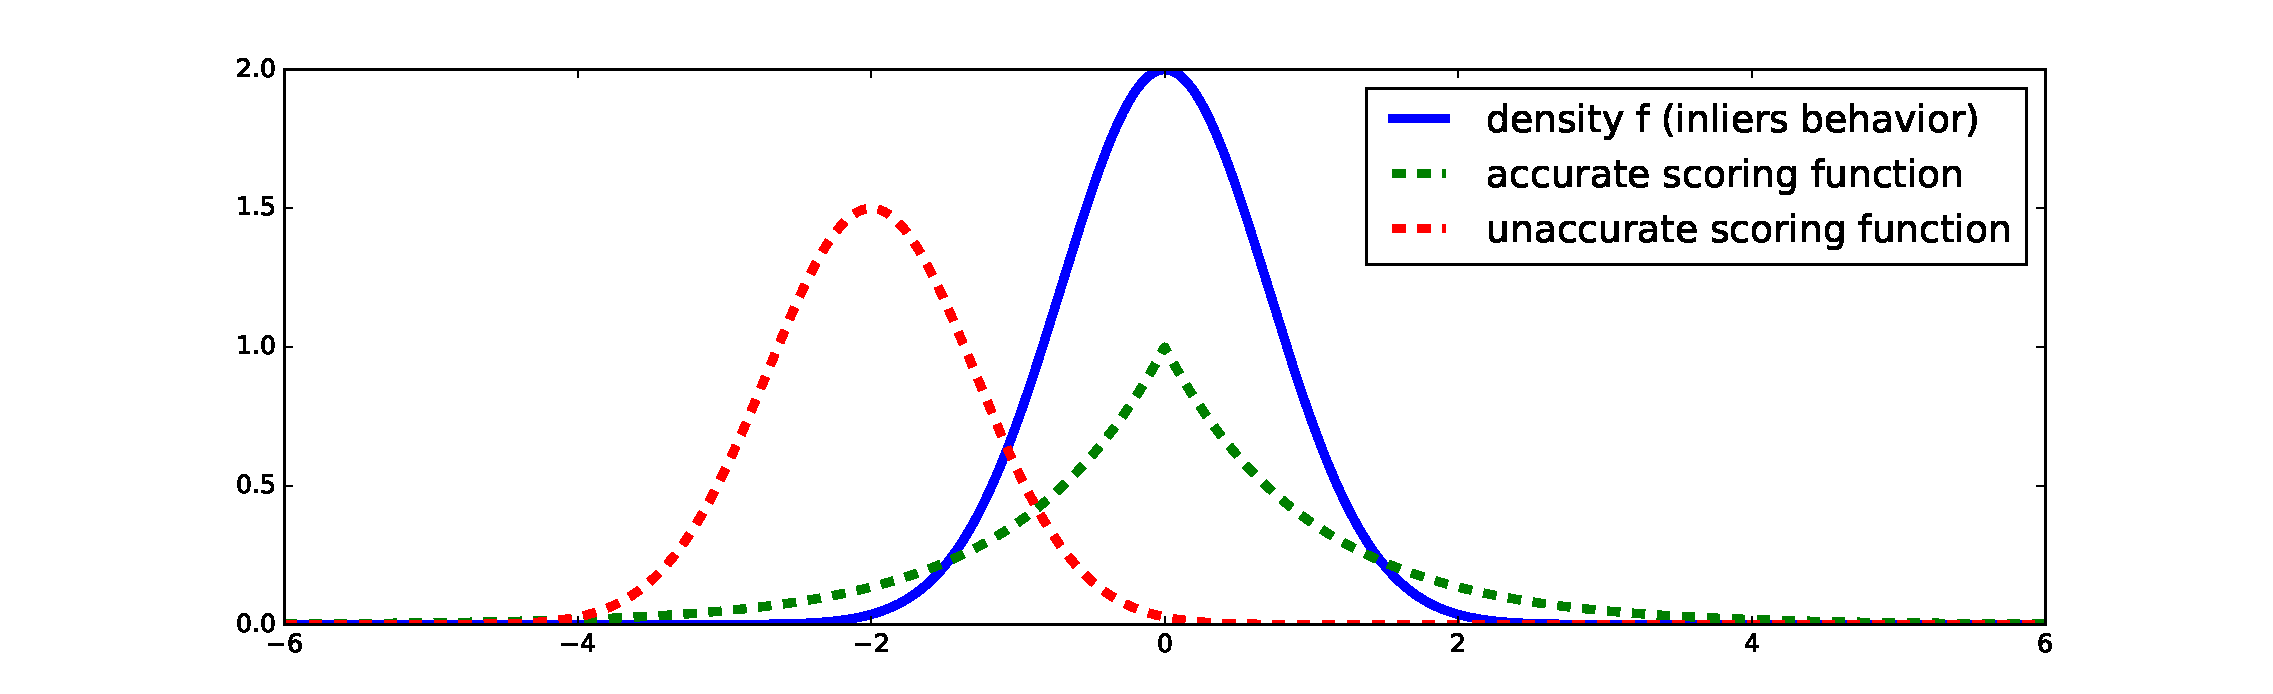
\includegraphics[width=1.01\columnwidth]{sourcefigs/scoring.pdf}
\end{figure}

\end{frame}




% \begin{frame}
% \frametitle{Contributions and Outline}

% \begin{block}{Contributions}

% \begin{itemize}
% \item Performance criterion for learning scoring functions: Excess-Mass Curve (Part I).

% \item Learning scoring functions on extreme regions (Part II).

% \item Evaluating scoring functions in non-small dimensions (Part I).

% \item One-class splitting criteria for Random Forests. (not in this presentation)
% \end{itemize}
 
% \end{block}

% \end{frame}


% \begin{frame}
% \frametitle{Outline}
% %In a machine learning context, AD can been seen as a classification task but where the usual assumption -dataset contains info regarding all classes- breaks down.

% \begin{block}{}
% \begin{itemize}
% \item Part I: Performance criterion on {\blue $s$}.\\
% {\footnotesize ~~(model selection)} \\~\\~\\
% %{\small ~~~~~~~~~~~~ $\to$ Evaluation criterion for AD algorithms.}\\~\\~\\~\\
% \item Part II: Building good {\blue $s$} on extreme regions. \\
% {\footnotesize ~~ (model design)}
% %{\small ~~~~~~~~~~~~ $\to$ Gaining in accuracy on extreme regions.}
% \end{itemize}
% \end{block}
% \end{frame}

\begin{frame}
\frametitle{Outline}
\tableofcontents
\end{frame}


\section{Part I: Performance criterion for scoring functions}
% \subsection{Definition}




% \begin{frame}
% \frametitle{Context}
% %In a machine learning context, AD can been seen as a classification task but where the usual assumption -dataset contains info regarding all classes- breaks down.

% \begin{block}{Novelty Detection { \footnotesize (`One-Class Classification', `semi-supervised AD')}}~\\~\\

% \begin{itemize}
% \item \textbf{Data: {\red inliers}}.\\
% i.i.d. observations in $\mathbb{R}^d$ from the normal behavior, density {\red $f$}.\\~\\
% %{\footnotesize Remark: In practice, data can be polluted by a small proportion of anomalies.}

% \item \textbf{Output to evaluate: {\blue scoring function $s: \mathbb{R}^d \to \mathbb{R}$}} \\
% %{\footnotesize
% %- AD algorithms return {\blue $s: \mathbb{R}^d \to \mathbb{R}$}.\\
% - $s$ defines a {\blue pre-order} on $\mathbb{R}^d$ = `degree of abnormality'.\\
% - $s$ level sets are estimates of $f$ level sets.\\
% - $s$ can be interpreted as a box which contains {\blue an infinite number of level sets estimates} (at different levels).\\~\\
% \end{itemize}

% \textbf{Remark.} Ideal scoring functions: $s=f$ or $s=2f+3$ or $s=T \circ f$ any increasing transform of $f$. \\
% %($f=2s$, $f=s^2$ if $s \ge 0$, ...).

% \end{block}
% \end{frame}


% \begin{frame}
% \frametitle{Problem reformulation}
% We want a criterion $\mathcal{C}(s)$ which measures \emph{how well the level sets of $f$ are approximated by those of $s$}.
% %$$\mathcal{C}(s) (t) \simeq ~\inf_{u>0}~ \leb(\{ s >u\}~\Delta~\{f>t\})$$
% \begin{block}{}
% \begin{itemize}
% \item \textbf{Fact:} For any strictly increasing transform $T$, level sets of $T \circ f$ are exactly those of $f$.\\
% $\Rightarrow$ Criterion $\mathcal{C}(s) = \|s-f\|$ is not relevant! ($\mathcal{C}(2f) > 0$)\\~\\

% \item \textbf{We are looking for a criterion s.t:}\\
% - $\crit^{\Phi}(s) = \| \Phi(s) - \Phi(f) \|$ with $\Phi$ s.t. $\Phi(T \circ s) = \Phi(s)$. \\
% - $ \{ \text{level sets of optimal }~ s^*\} = \{ \text{level sets of } ~f \}$. \\
% - $\crit^{\Phi}(s)$ = `distance' between level sets of $s$ and those of $f$.

% \end{itemize}
% \end{block}
%  % $\Rightarrow \Phi(s) := MV_s$ or $EM_s$, the Mass-Volume and Excess-Mass curves of $s$.
% Question: How to choose $\Phi(s)$ ?
% \end{frame}


\begin{frame}
\frametitle{Existing criterion: Mass-Volume curve}
% For a random variable $\mb X$, \emph{normal region}: region of minimum volume among all regions with probability greater than $\alpha \in (0,1)$.\\~\\

\begin{minipage}{0.6\textwidth}
	{\blue Minimum volume set} {\small [Einmahl and Mason 1992, Polonik 1997]}
	\begin{equation*}
	\Gamma^*_{\alpha} = \argmin_{\Gamma\text{ borelian} } ~~~\text{Leb}(\Gamma)~~~s.t.~~~ \mathbb{P}(\mb X \in \Gamma) \geq \alpha
	\end{equation*}
\end{minipage}
\begin{minipage}{0.3\textwidth}
	\centering
	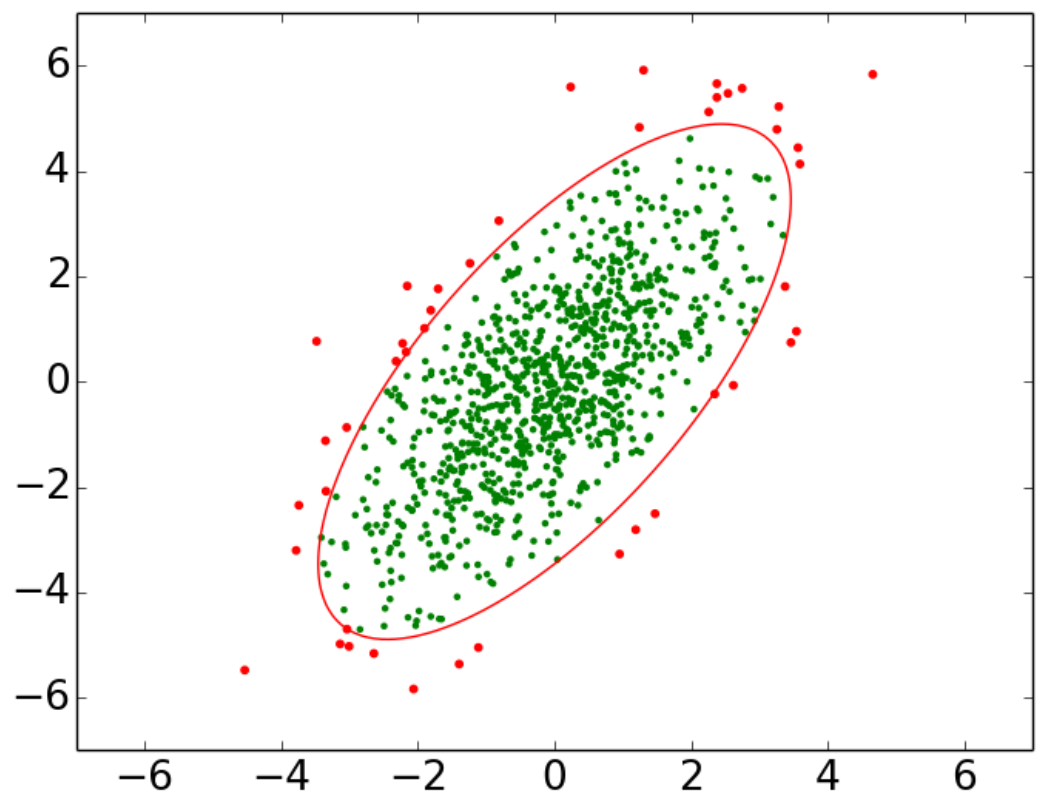
\includegraphics[width=0.95\textwidth]{img/anomaly_detection_end_col.png}
\end{minipage}

% Under regularity assumptions, minimum-volume sets are \textbf{density level sets}:
% $$\exists t_\alpha>0,~~~ \Gamma^*_{\alpha} = \{f > t_\alpha\} =: \Omega_{t_\alpha} $$

{\blue Mass Volume curve} of a scoring function $s$ {\small [Clémençon and Jakubowicz, 2013]}:
% \footnotesize{
\begin{align*}
MV_s(\alpha) ~:&=~ \inf_{\Gamma \text{ level-set of } s} \big\{~ \leb(\Gamma) ~~~s.t.~~ \mathbb{P}(\mb X \in \Gamma) \ge \alpha~\big\} \\
MV^*(\alpha) ~:&=~ MV_f(\alpha) %\overset{prop}{=}  \min_{\Gamma~ \text{borelian}} \big\{~\leb(\Gamma) ~~~\st~~ \mathbb{P}(\mb X \in \Gamma) \ge \alpha ~\big\} 
\end{align*}
%
\begin{figure}[htb]
\centering
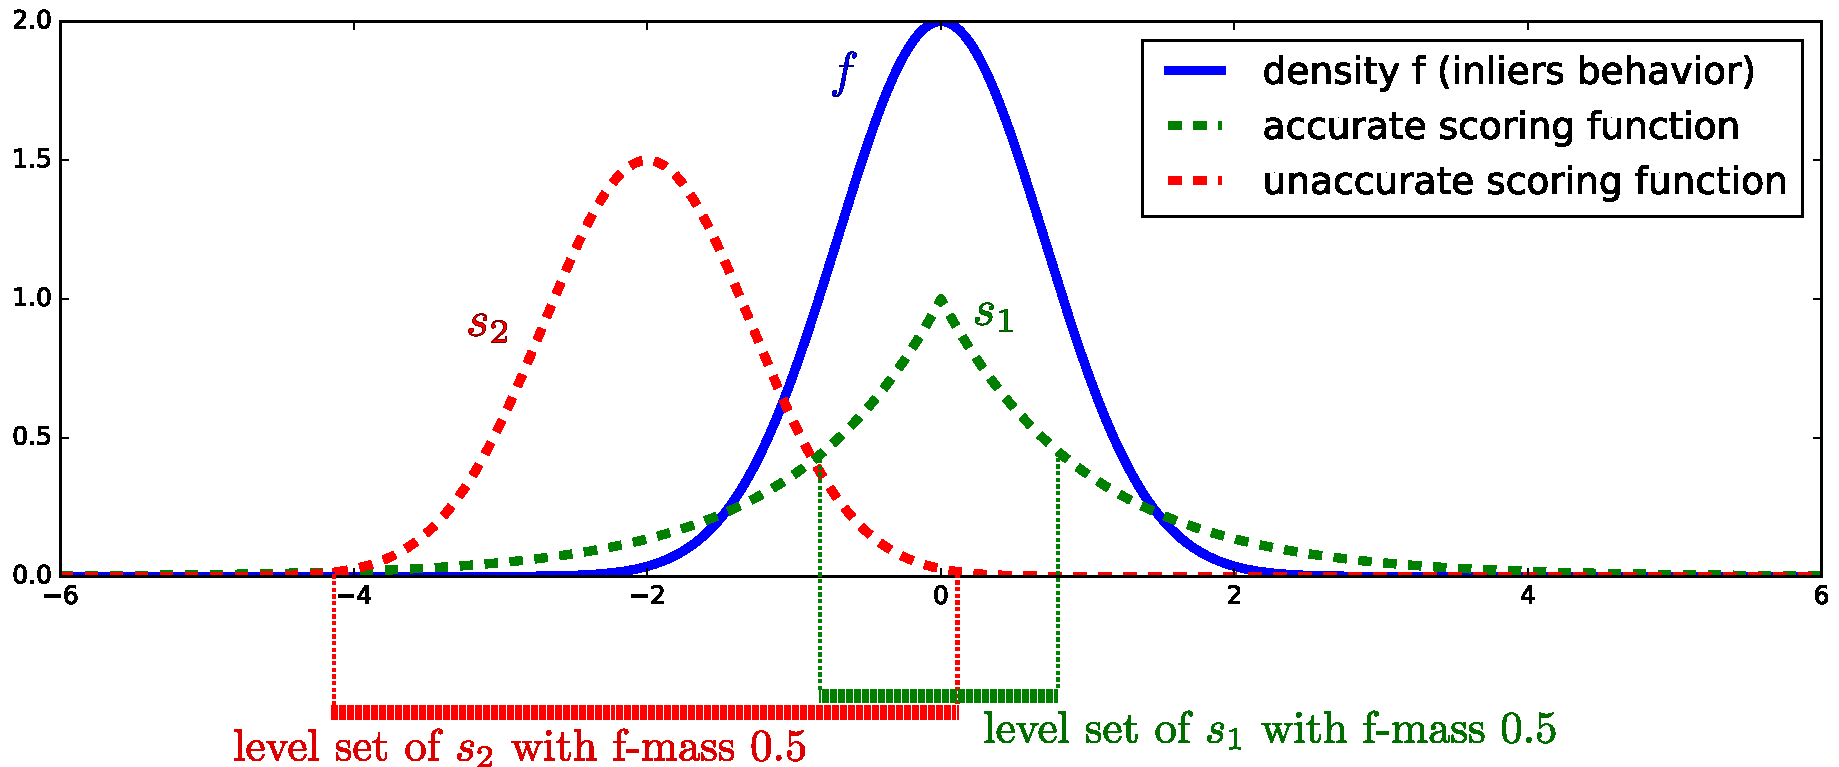
\includegraphics[width=0.87\columnwidth]{sourcefigs/scoring2.pdf}
\end{figure}

\end{frame}


% \begin{frame}\frametitle{Existing criterion: Mass-Volume curve}

% Properties:

% \begin{itemize}
% \item For any scoring function $s$, $MV^*(\alpha) \le MV_s(\alpha)$
% \item For any increasing transform $T$, $MV^*(\alpha)  = MV_{T \circ f}(\alpha)$
% \item $MV^*(\alpha) = \text{Leb}(\Gamma_\alpha^*) := \min_{\Omega~ \text{borelian}} ~\big\{\leb(\Omega) ~~~\st~~ \mathbb{P}(\mb X \in \Omega) \ge \alpha\big\}$\\~\\
% ($MV_s(\alpha) ~:=~ \inf_{\Omega \text{ level-set of } s}~~~ \big\{\leb(\Omega) ~~~~s.t.~~~~ \mathbb{P}(\mb X \in \Omega) \ge \alpha\big\}
% $)
% \end{itemize}


% \begin{figure}[htb]
% \centering
% \subfigure[Scoring functions]{%
% 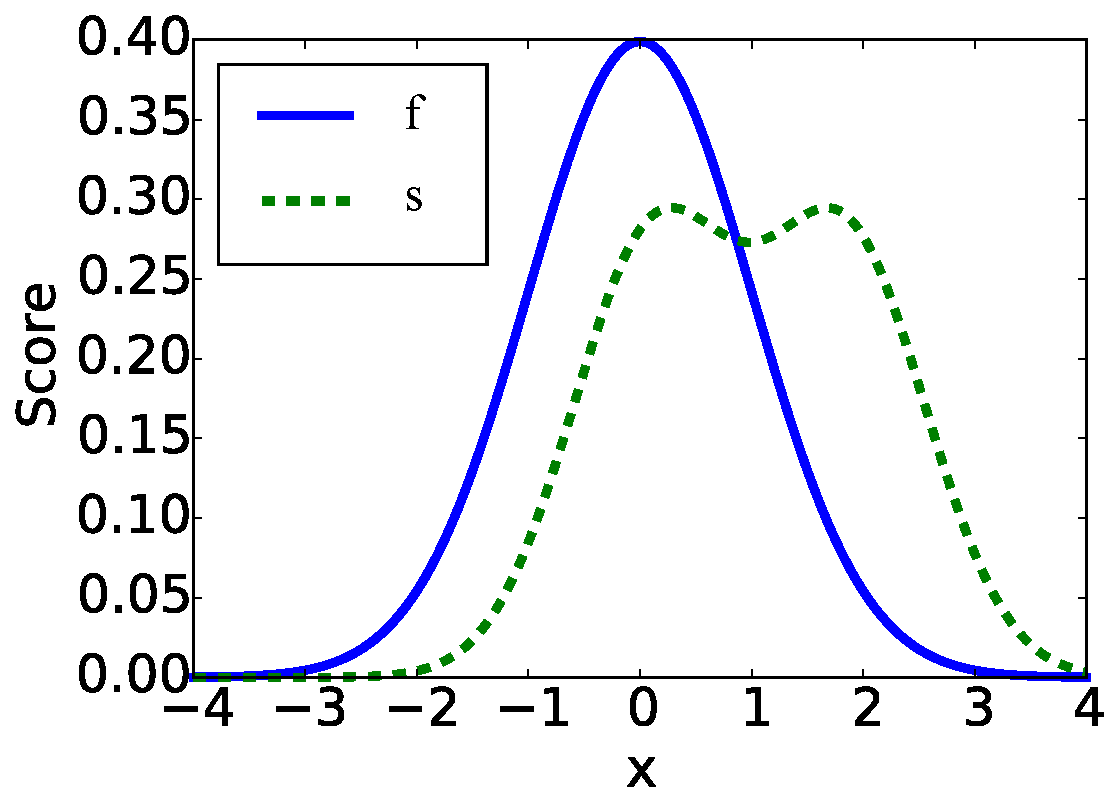
\includegraphics[width=0.45\columnwidth]{img/mv_curves_examples_1_comp_inkscape.pdf}}
% \subfigure[Mass Volume curves]{%
% 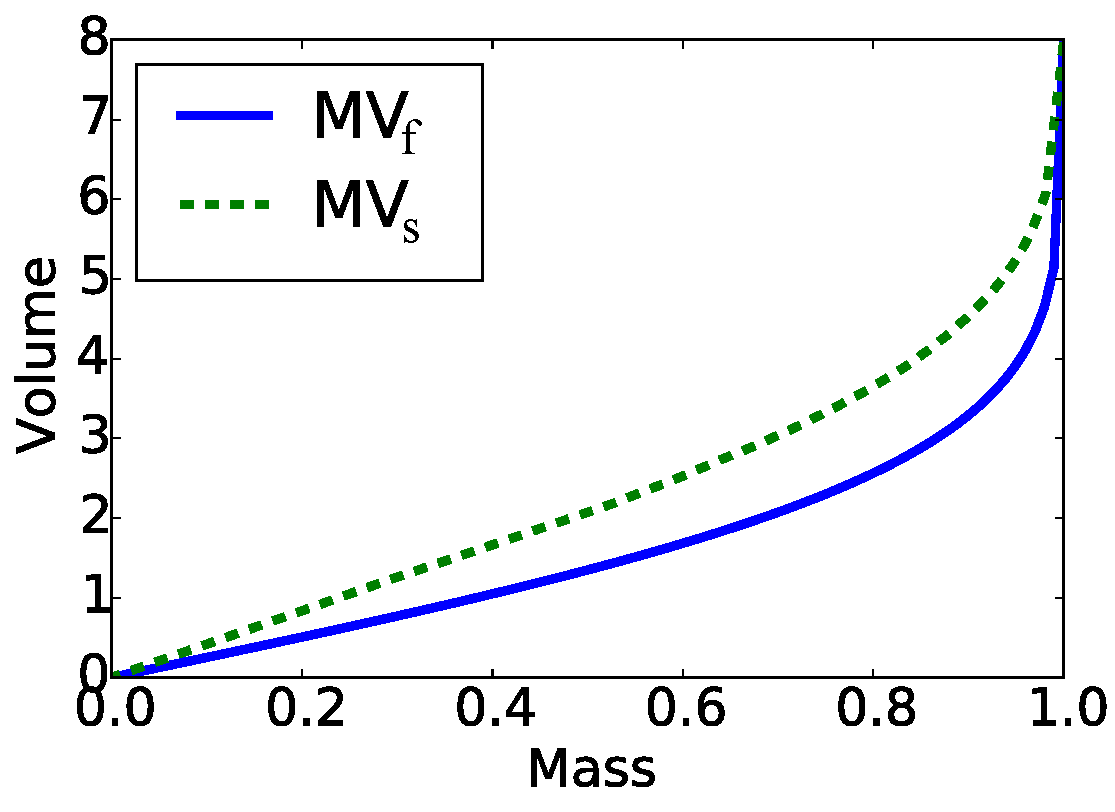
\includegraphics[width=0.45\columnwidth]{img/mv_curves_examples_2_comp_inkscape.pdf}}
% \end{figure}


% \end{frame}



\begin{frame}
\frametitle{Existing criterion: Mass-Volume curve}
\begin{figure}
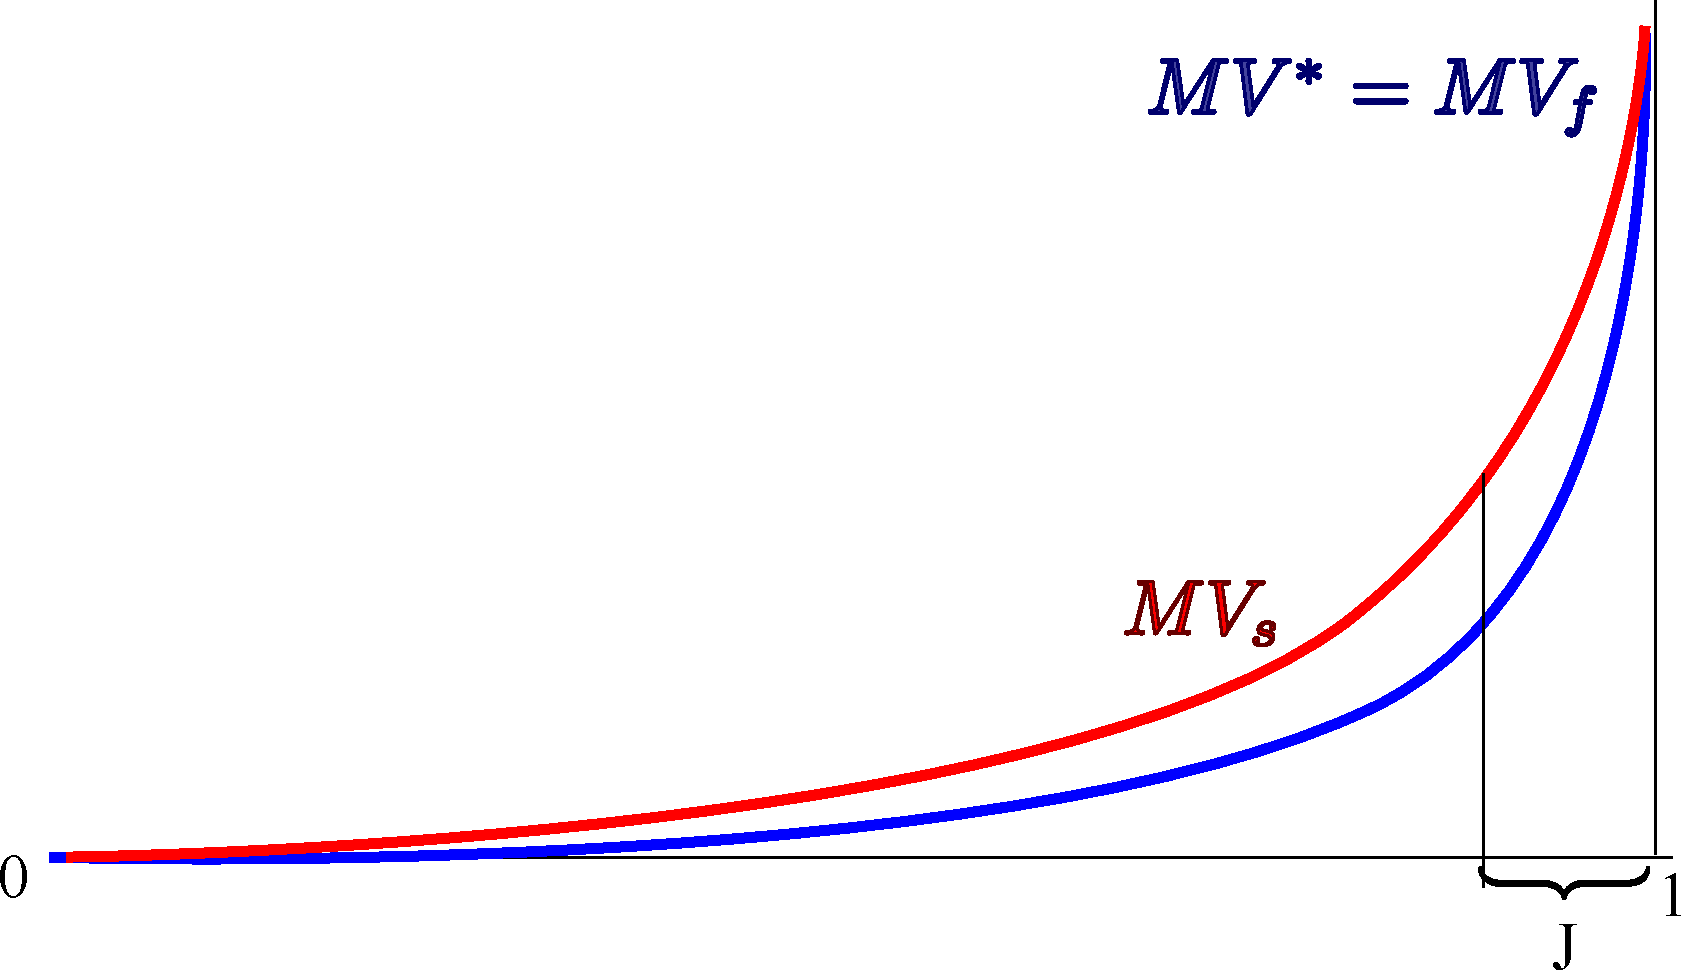
\includegraphics[width = 0.7\linewidth]{sourcefigs/mv.pdf}
\end{figure}

Main drawbacks of MV:
\begin{itemize}
\item When optimized \emph{w.r.t.} different levels $\alpha$ over a finite class, produces \textbf{not necessarily nested} empirical level sets.
\item $\to$ \textbf{low convergence rates} -- of order $O(n^{-1/4})$.
\item MV \textbf{diverges} in $1$ in case of unbounded support.
\end{itemize}

\end{frame}

\begin{frame}
\frametitle{Our contribution: Excess-Mass curve  {\small [Goix, Sabourin, Clémençon 2015]}}

Excess-Mass {\small [Hartigan 1987, Polonik 1995]}\\
{\blue \large Excess-Mass curve }
\begin{align*}
EM_s(t) ~~:&=~ \sup_{\Omega \text{ level-set of } s}~~~\big\{ \mathbb{P}(\mb X \in \Omega) ~-~ t \leb(\Omega) \big\}\\
EM^*(t) ~~:&=~  EM_f(t) %\overset{prop}{=}  \max_{\Omega\text{ borelian} } ~\big\{{\mathbb{P}} (\mb X\in \Omega)-t\leb(\Omega) \big\} 
%&EM^*(t) \ge EM_s(t)~~~~~~~~~~~~\text{for all scoring function}~~ s
\end{align*}

\begin{alertblock}{Property: Previous drawbacks are fixed with EM.}
\begin{itemize}
\item Produces \textbf{nested} empirical level sets.
\item $\to$ \textbf{convergence rates} of order $O(n^{-1/2})$.
\item EM curve \textbf{finite} even in case of unbounded support.
\end{itemize}
\end{alertblock}


\begin{figure}
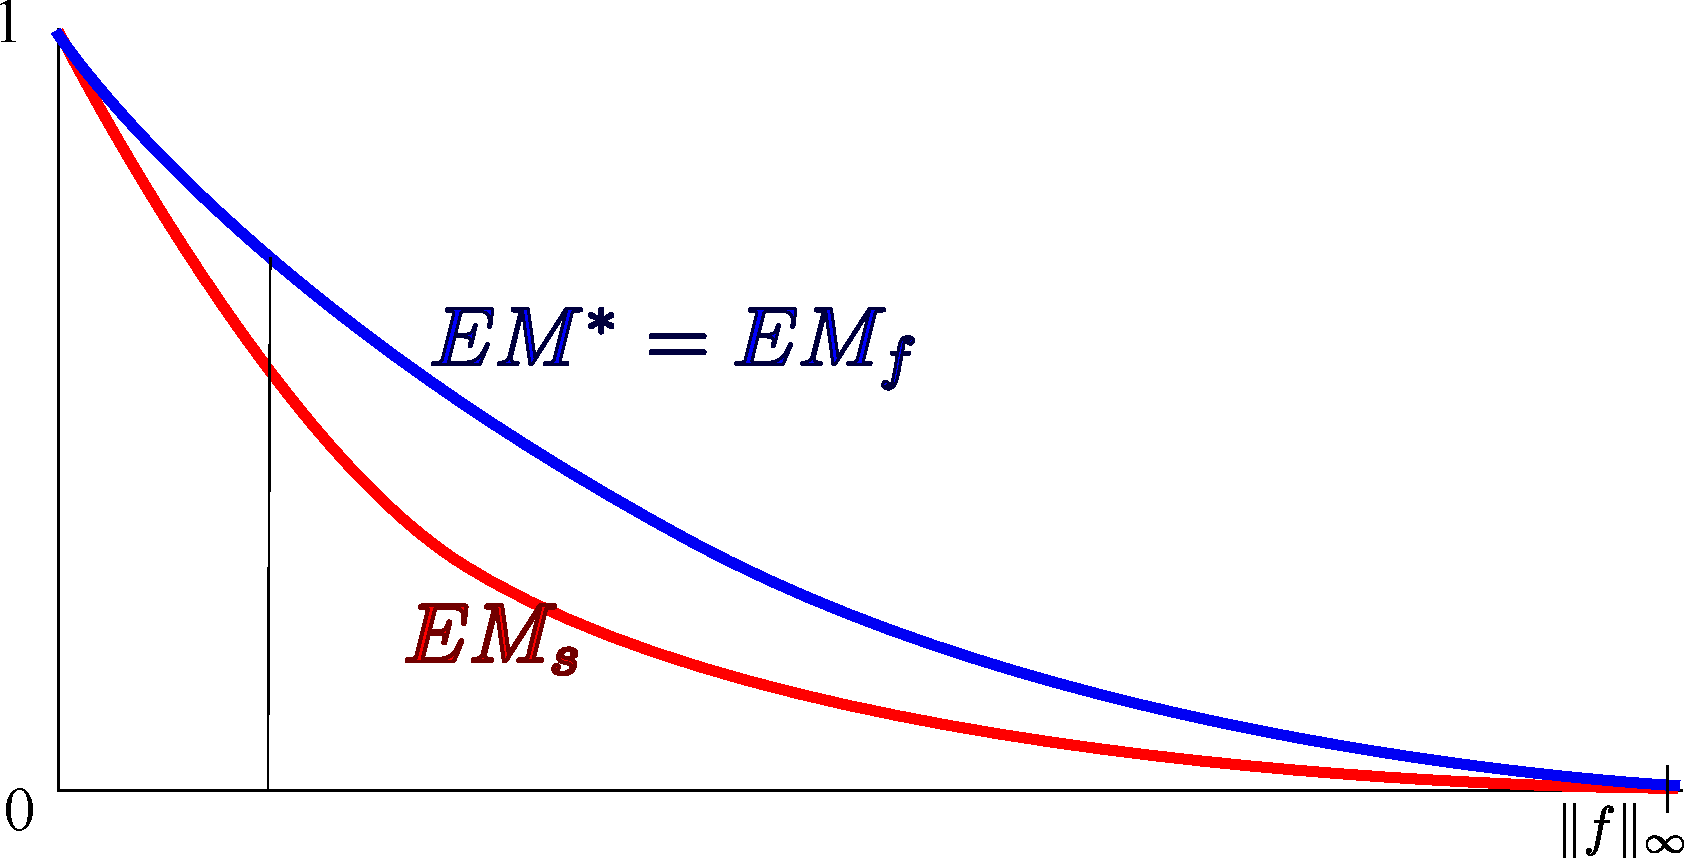
\includegraphics[width = 0.6\linewidth]{sourcefigs/em.pdf}
\end{figure}


\end{frame}


% \begin{frame}
% \frametitle{MV and EM criteria}
% \begin{itemize}
% \item \textbf{Interpretation:} $(EM_f - EM_s)(t) \simeq ~\inf_{u>0}~ \leb(\{ s >u\}~\Delta~\{f>t\})$ \\~\\~\\
% % \begin{align*}
% % &\| EM_s - EM_f\|_{L^1(I)} : \text{ how well $t$-level sets of $f$ are approximated by}\\
% % &~~~~~~~~~~~~~~~~~~~~~~~~~~~~~~~~~~\text{ level sets of $s$, $t \in I$}.\\
% % &\| MV_s - MV_f\|_{L^1(J)} : \text{ how well $\alpha$-level sets of $f$ are approximated by} \\
% % &~~~~~~~~~~~~~~~~~~~~~~~~~~~~~~~~~~\text{ level sets of $s$, $\alpha \in J$}.\\
% % %&(EM_s - EM_f)(t) \simeq \inf_{u>0} Leb (\{ s >u\}\Delta\{f>t\})
% % \end{align*}


% \item How well {\red $t$}-level sets of $f$ are approximated by level sets of $s$, ${\red t} \in I$ ? \\
% {\centering $\updownarrow$\\
% how {\blue small} is $EM_f - EM_s$ on $I$ ? \\$\updownarrow$\\
% ~~~~~~~~~~~~~~~~~~~~~~~~~~~\textbf{how {\blue large} is $EM_s$ on $I$ ?} ~~~~$\to$  {\red $\mathcal{C}^{EM}(s) = \|EM_s\|_{1, I}$}  \\~\\~\\}

% \item How well {\red $\alpha$} minimum-volume sets of $f$ are approximated by level sets of $s$, ${\red \alpha} \in J$ ? \\
% {\centering $\updownarrow$\\
%  how {\blue small} is $MV_s - MV_f$ on $J$ ? \\
% $\updownarrow$\\
% ~~~~~~~~~~~~~~~~~~~~~~~~~\textbf{how {\blue small} is $MV_s$ on $J$ ?} ~~~$\to$  {\red $\mathcal{C}^{MV}(s) = \|MV_s\|_{1, J}$}
% }
 
% \end{itemize}


% \end{frame}


% \subsection{Learning a scoring function}

\begin{frame}
\frametitle{Learning a scoring function with M-estimation}



% We are looking for nearly optimal scoring functions of the form {\blue $s(x) = \sum_{j=1}^N a_j \mathds{1}_{x \in \Omega_j}$}, with $a_j \ge 0$,~ $\Omega_j \in \mathcal{G}$ a VC-class.\\

$\mathcal{G}$: VC-class of sets.

\begin{block}{}
{\blue Procedure}:  Fix $t_0 > 0$\\
For $k=1, \ldots, N$,
%
\begin{align*}
&t_{k+1} ~~=~ \frac{t_k}{(1 + \frac{1}{\sqrt n})}\\
&\widehat \Omega_{t_{k+1}} =~~ \argmax_{\Omega \in \mathcal{G},~ \widehat \Omega_{t_k} \subset \Omega } ~~~~ \mathbb{P}_n(X \in \Omega) ~-~ t_{k+1} \leb(\Omega)
\end{align*}
%
%where $\mathbb{P}_n(X \in \Omega) = \frac{1}{n} \sum_{i=1}^n \mathds{1}_{X_i \in \Omega}$, we obtain
$s_N(x) := \sum_{j=1}^N(t_j - t_{j+1}) \mathds{1}_{x \in \widehat \Omega_{t_j}}$
\begin{figure}
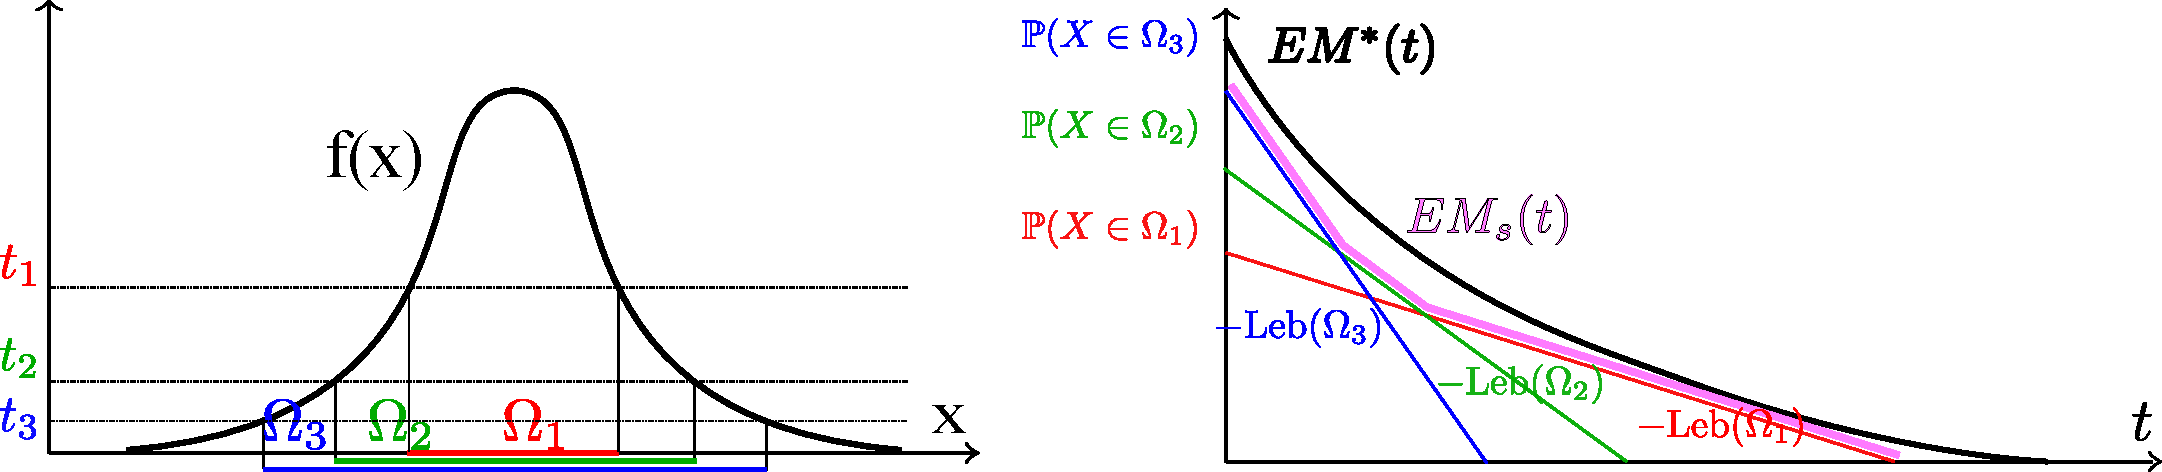
\includegraphics[width=0.5\linewidth]{sourcefigs/em_optim.pdf}
\end{figure}
\end{block}

\end{frame}

\begin{frame}
\frametitle{Learning a scoring function with M-estimation}

\begin{block}{Theorem}
Assume the density $f$ bounded, with compact support and without flat parts and $\mathcal{G}$ VC-class.
Then if $t_N = \mathcal{O}(n^{-1/2})$, with probability at least $1-\delta$, %(\eg~if $N \sim \sqrt n \log n$)
\begin{align*}
\sup_{t \in ]0,t_1]}|EM^*(t)-EM_{s_N}(t)| ~\le~ \left[A+\sqrt{2\log(1/\delta)}\right]\frac{1}{\sqrt n}+ bias(\mathcal{G}). %+ o_N(1).
\end{align*}
\end{block}
~\\~\\~\\~\\~\\~\\
\begin{figure}
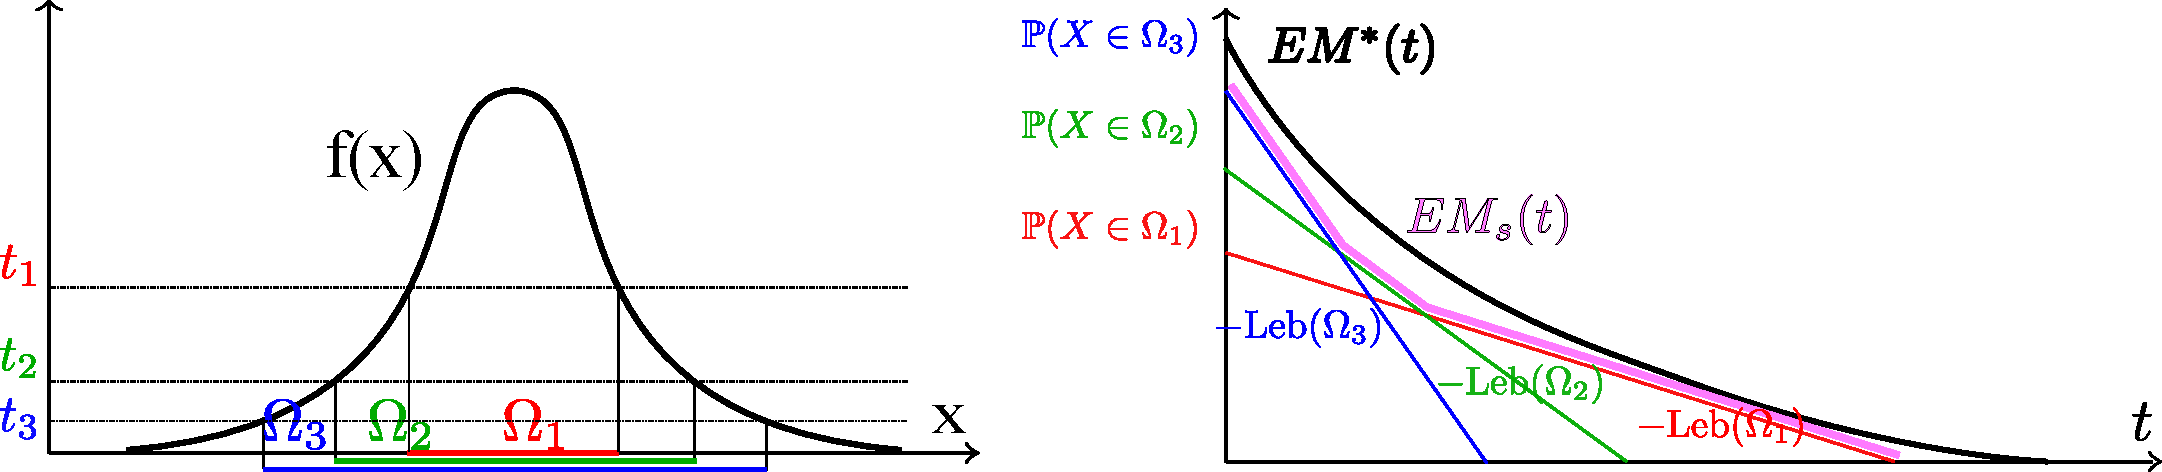
\includegraphics[width=0.5\linewidth]{sourcefigs/em_optim.pdf}
\end{figure}

\end{frame}


\section{Part II: Learning accurate scoring functions on extreme regions}



% \subsection{Multivariate EVT \& Representation of Extremes}

\begin{frame}
\frametitle{Why dealing with extremes?}
\begin{alertblock}{General ideas:}
\begin{itemize}
\item Extreme observations play a special role when dealing with outlying data.\\~\\
\item But no anomaly detection algorithm has \textbf{specific treatment for such multivariate extreme observations}. Univariate EVT: [Roberts 99, Lee and Roberts 2008, Clifton \emph{et al.} 2011]\\~\\
\item Our goal:
  \begin{itemize}
  \item Define a notion of sparsity for extremes observations.
  \item Provide a method which can improve performance of standard AD algorithms by combining them with a \textbf{multivariate extreme analysis} of the \textbf{dependence structure}, using this notion of sparsity.
  \end{itemize}
\end{itemize}
\end{alertblock}
\end{frame}

% \begin{frame}
% \begin{figure}
% \centering
% 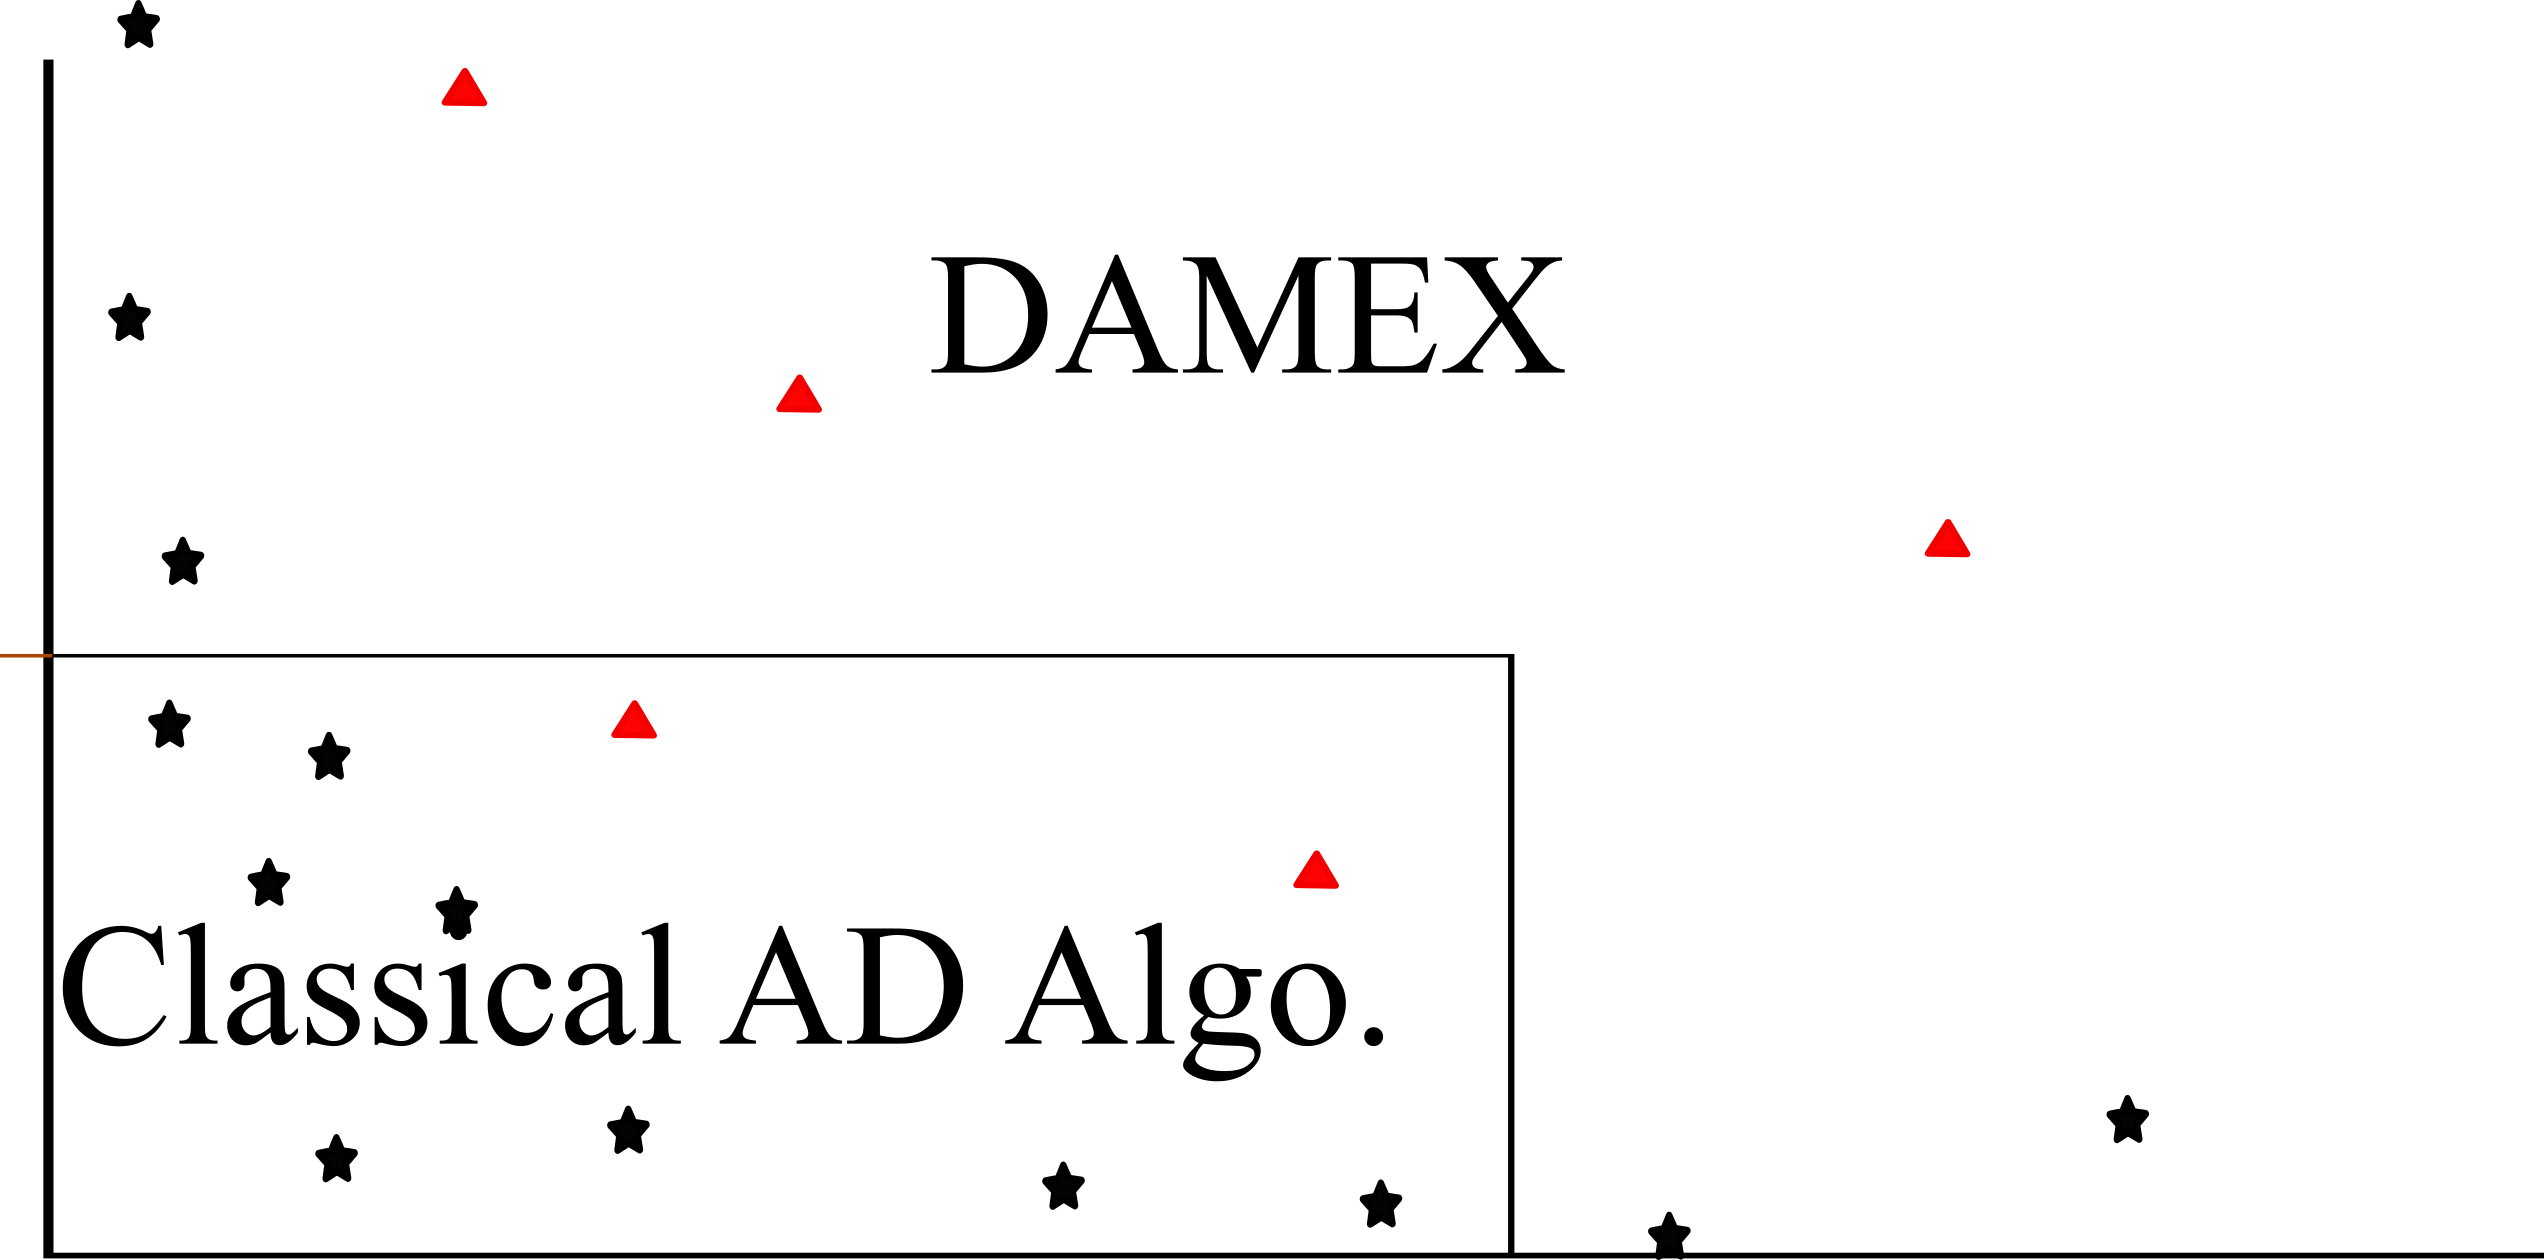
\includegraphics[height=3.5cm]{sourcefigs/extreme_AD.png}
% \end{figure}
% \end{frame}


\begin{frame}
\frametitle{Purpose}
\noindent
\begin{align*}
\mb X = (X_1,\ldots,X_5)
\end{align*}
~\\
{\large Goal: find the groups of features which can be large together}
\begin{align*}
\text{ex:~~~~}\{X_1, X_2\},~\{X_1, X_3, X_4\},~\{X_5\}
\end{align*}
~\\~\\
{\large Namely: characterize the extreme dependence structure\\~\\~\\

$\to$ Anomalies~~=~~ points which violate this structure
}
\end{frame}



\begin{frame}
\frametitle{Theoretical framework}
\begin{itemize}
\item \textbf{Context} 

  \begin{itemize}
  \item Random vector    $  \mb X = (X_{1},\ldots,X_{d})  $
    \vspace{0.3cm}
  \item Margins: $X_{j}\sim F_j$ ~~~~~~~~~($F_j$ continuous)\\
    \vspace{0.3cm}
  \end{itemize}
    \vspace{0.3cm}

\item \textbf{Preliminary step: Standardization of each marginal}\\
    \vspace{0.3cm}
    \begin{itemize}
    \item   Standard Pareto: 
    $V_{j} = \frac{1}{1- F_j (X_{j})} $  ~~~~\Big($\mathbb{P}(V_j \ge x) = \frac{1}{x}$,~~ $x\ge 1$\Big) \\
    \end{itemize}
% OR\\
%     \vspace{0.3cm}

%   \item Uniform:
%     $U_{j} = 1- F_j (X_{j}) $
%     \vspace{0.3cm}


\end{itemize}

\end{frame}


\begin{frame}
\frametitle{Problematic of Extreme Value Theory}
\vspace{0.2cm}
Describe $\mb V$'s distribution, when $\mb V$ exceeds some large threshold.
\vspace{0.2cm}
    $$
    \mathbb{P}(\mb V\in A) = \text{?} ~~~~~~~~~~~~ (A  \text{ `far from the origin'}).
    $$
  \begin{figure}
    \centering
    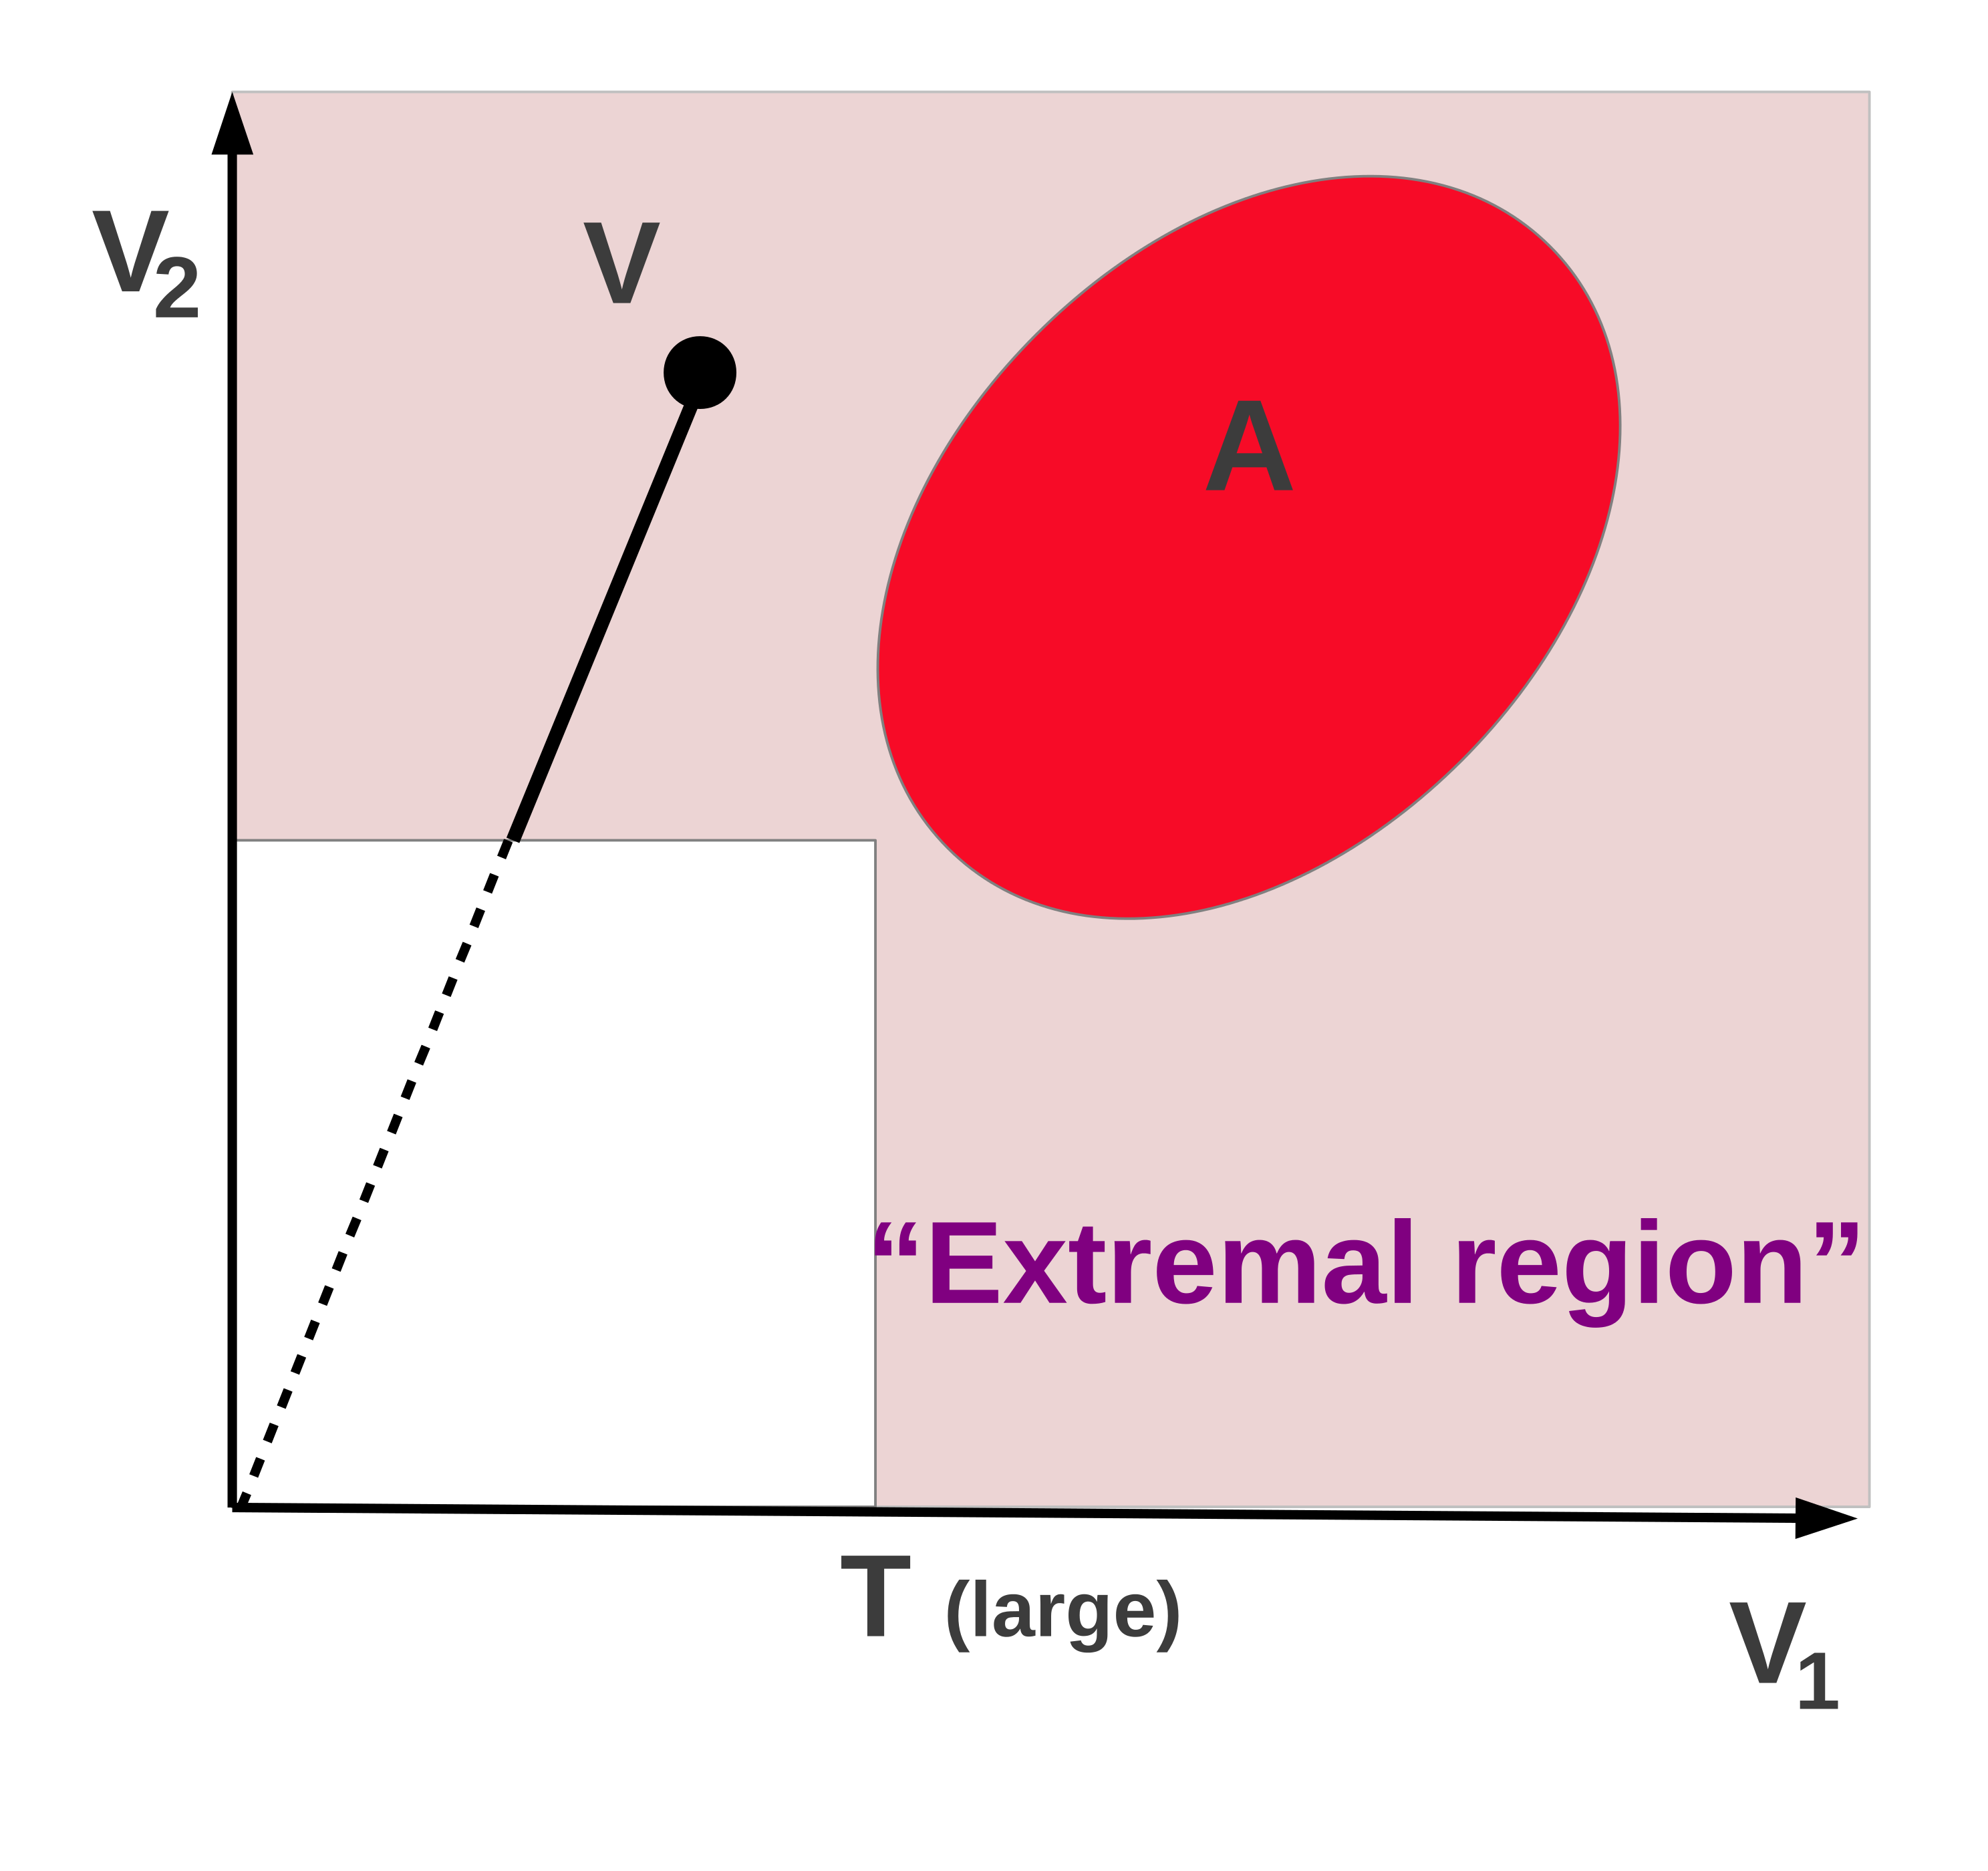
\includegraphics[scale=0.3]{sourcefigs/application4.png}
  \end{figure}
\end{frame}

\begin{frame}
  \frametitle{Fundamental hypothesis and consequences}%, fundamental result}

  \begin{itemize}
\item Standard assumption: let $A$ extreme region, $$\mathbb{P}[\mb V\in t~A] \simeq t^{-1}\mathbb{P}[\mb V\in A] \quad \text{(radial homogeneity)} $$ 
\item Formally:
\begin{exampleblock}{\textbf{regular variation} (after standardization):}
  $$\text{If~~~} 0 \notin \overline A,~~~~~~~~ t \mathbb{P}[\mb V\in t~A]\xrightarrow[t\to\infty]{} \mu(A). ~~~~~~~~~~~~~~~~~~~~~~~~~~~~~~~~~~$$
~~~~~~~~~~~~~~~~~~~~~~~~~~~~~~~~~~~~~~~~~~~~~~~~~~~~~~~~~~~~$\mu$: exponent measure

\end{exampleblock}
   Necessarily: $\mu(tA) = t^{-1} \mu(A)$ 

\vspace*{1cm}
\item
 $\Rightarrow $ \textbf{angular measure} on sphere $\mb S_{d-1}$: 
    $ \Phi(B) =\mu\{t B, t\ge 1\} % \quad B\subset \mb S_{d-1}
    $ 
\end{itemize}
\end{frame}

\begin{frame}
\frametitle{General model of multivariate EVT}
%
% We have achieved our goal:~
$\mathbb{P} [\mb V \in A]~~\simeq~~\mu(A)$, ~~if $A$ extreme region.\\~\\

\begin{block}{ { Model} for excesses }
%~~~~~For an extreme region  A: $$ \mathbb{P}[ \mb V \in A ]  ~~\simeq~~  \mu(A) \text{~~,~} t \to \infty$$
For a large $r>0$ and a region $B$ on the unit sphere: $$ \mathbb{P}\left[\|\mb V\|> r  ,~~\mb{\frac{V}{\|V\|}} \in B \right]  ~~\underset{r \to \infty}{\sim}~~  \frac{1}{r}\,\Phi(B)  = \mu(\{t B, t\ge r\})$$
\end{block}
\vspace*{.5cm}
$\Rightarrow$ $\Phi$ (or $\mu$) \textbf{rules the joint distribution of extremes} (if margins are known).
\begin{figure}[h]
\centering
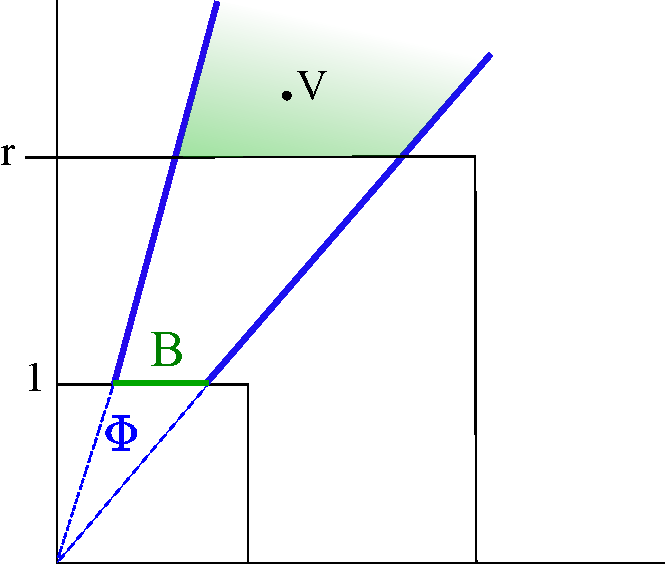
\includegraphics[width=0.4\linewidth]{sourcefigs/phi.pdf}
\end{figure}
\end{frame}




\begin{frame}
  \frametitle{Angular distribution}
$\Phi$ rules  the joint distribution of extremes:\\~\\
% end{itemize}
     \begin{figure}[h]
      \centering
      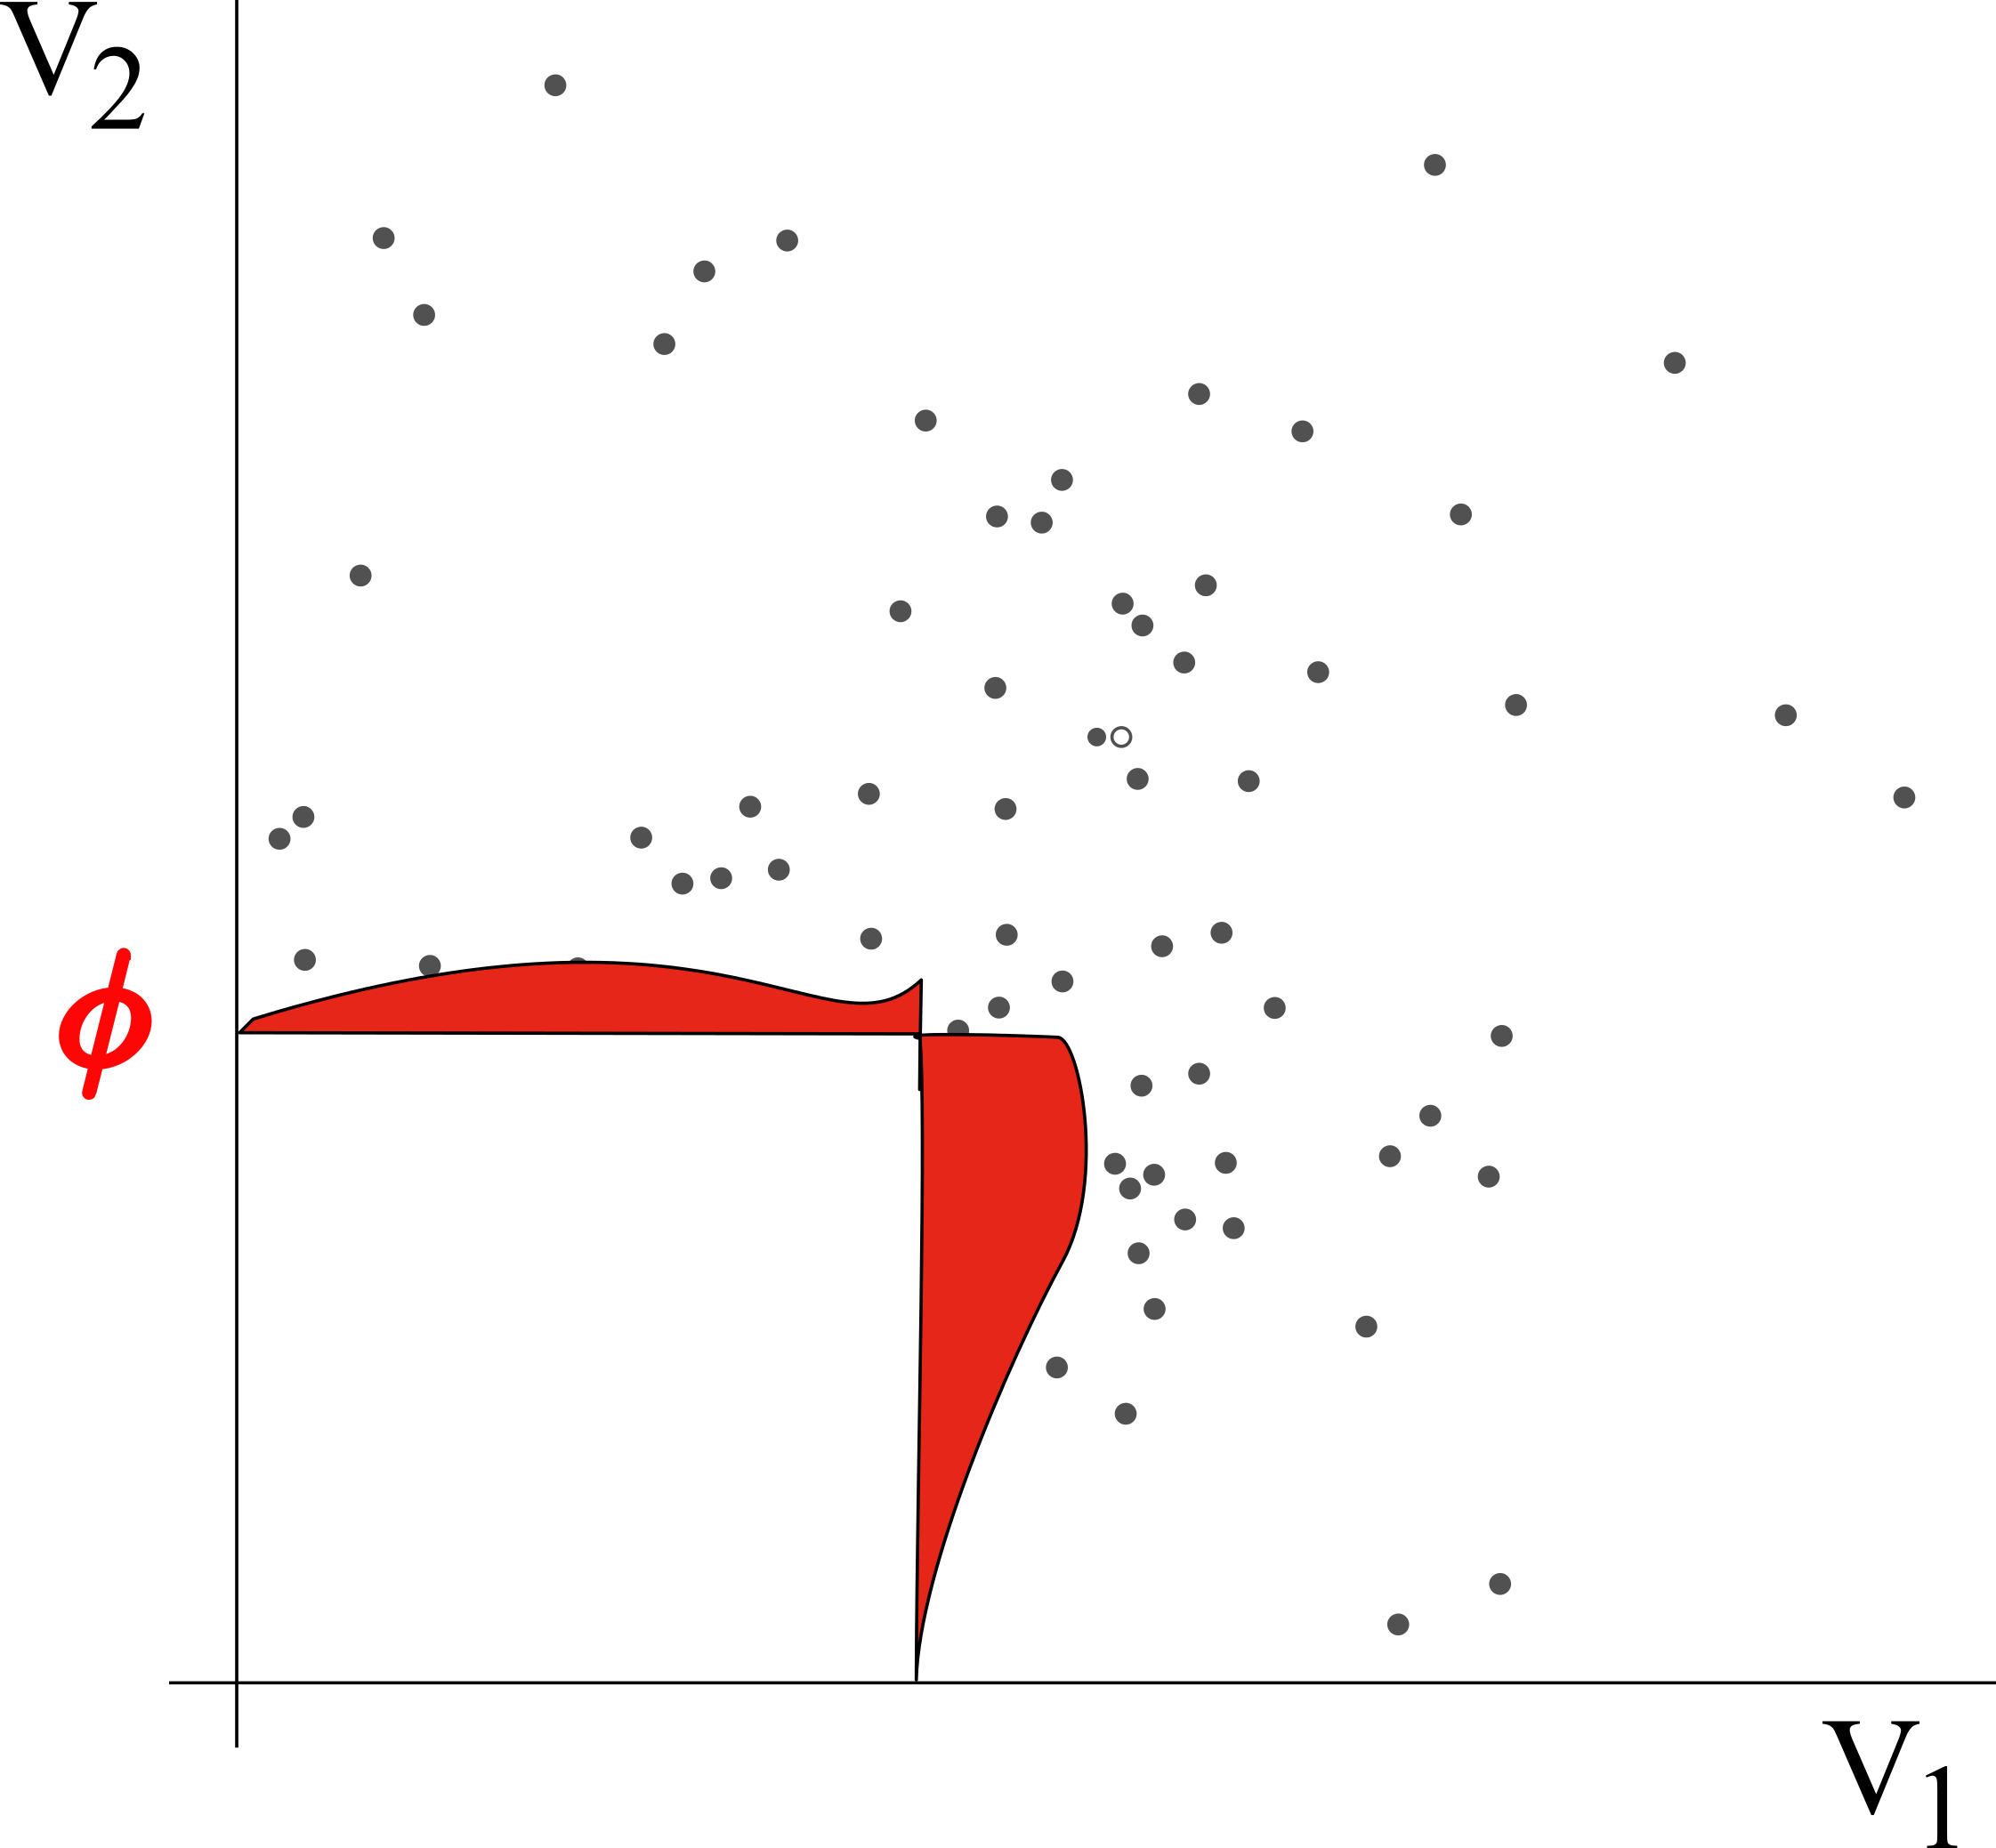
\includegraphics[scale=0.3]{sourcefigs/Example2D_depSquare.png}
      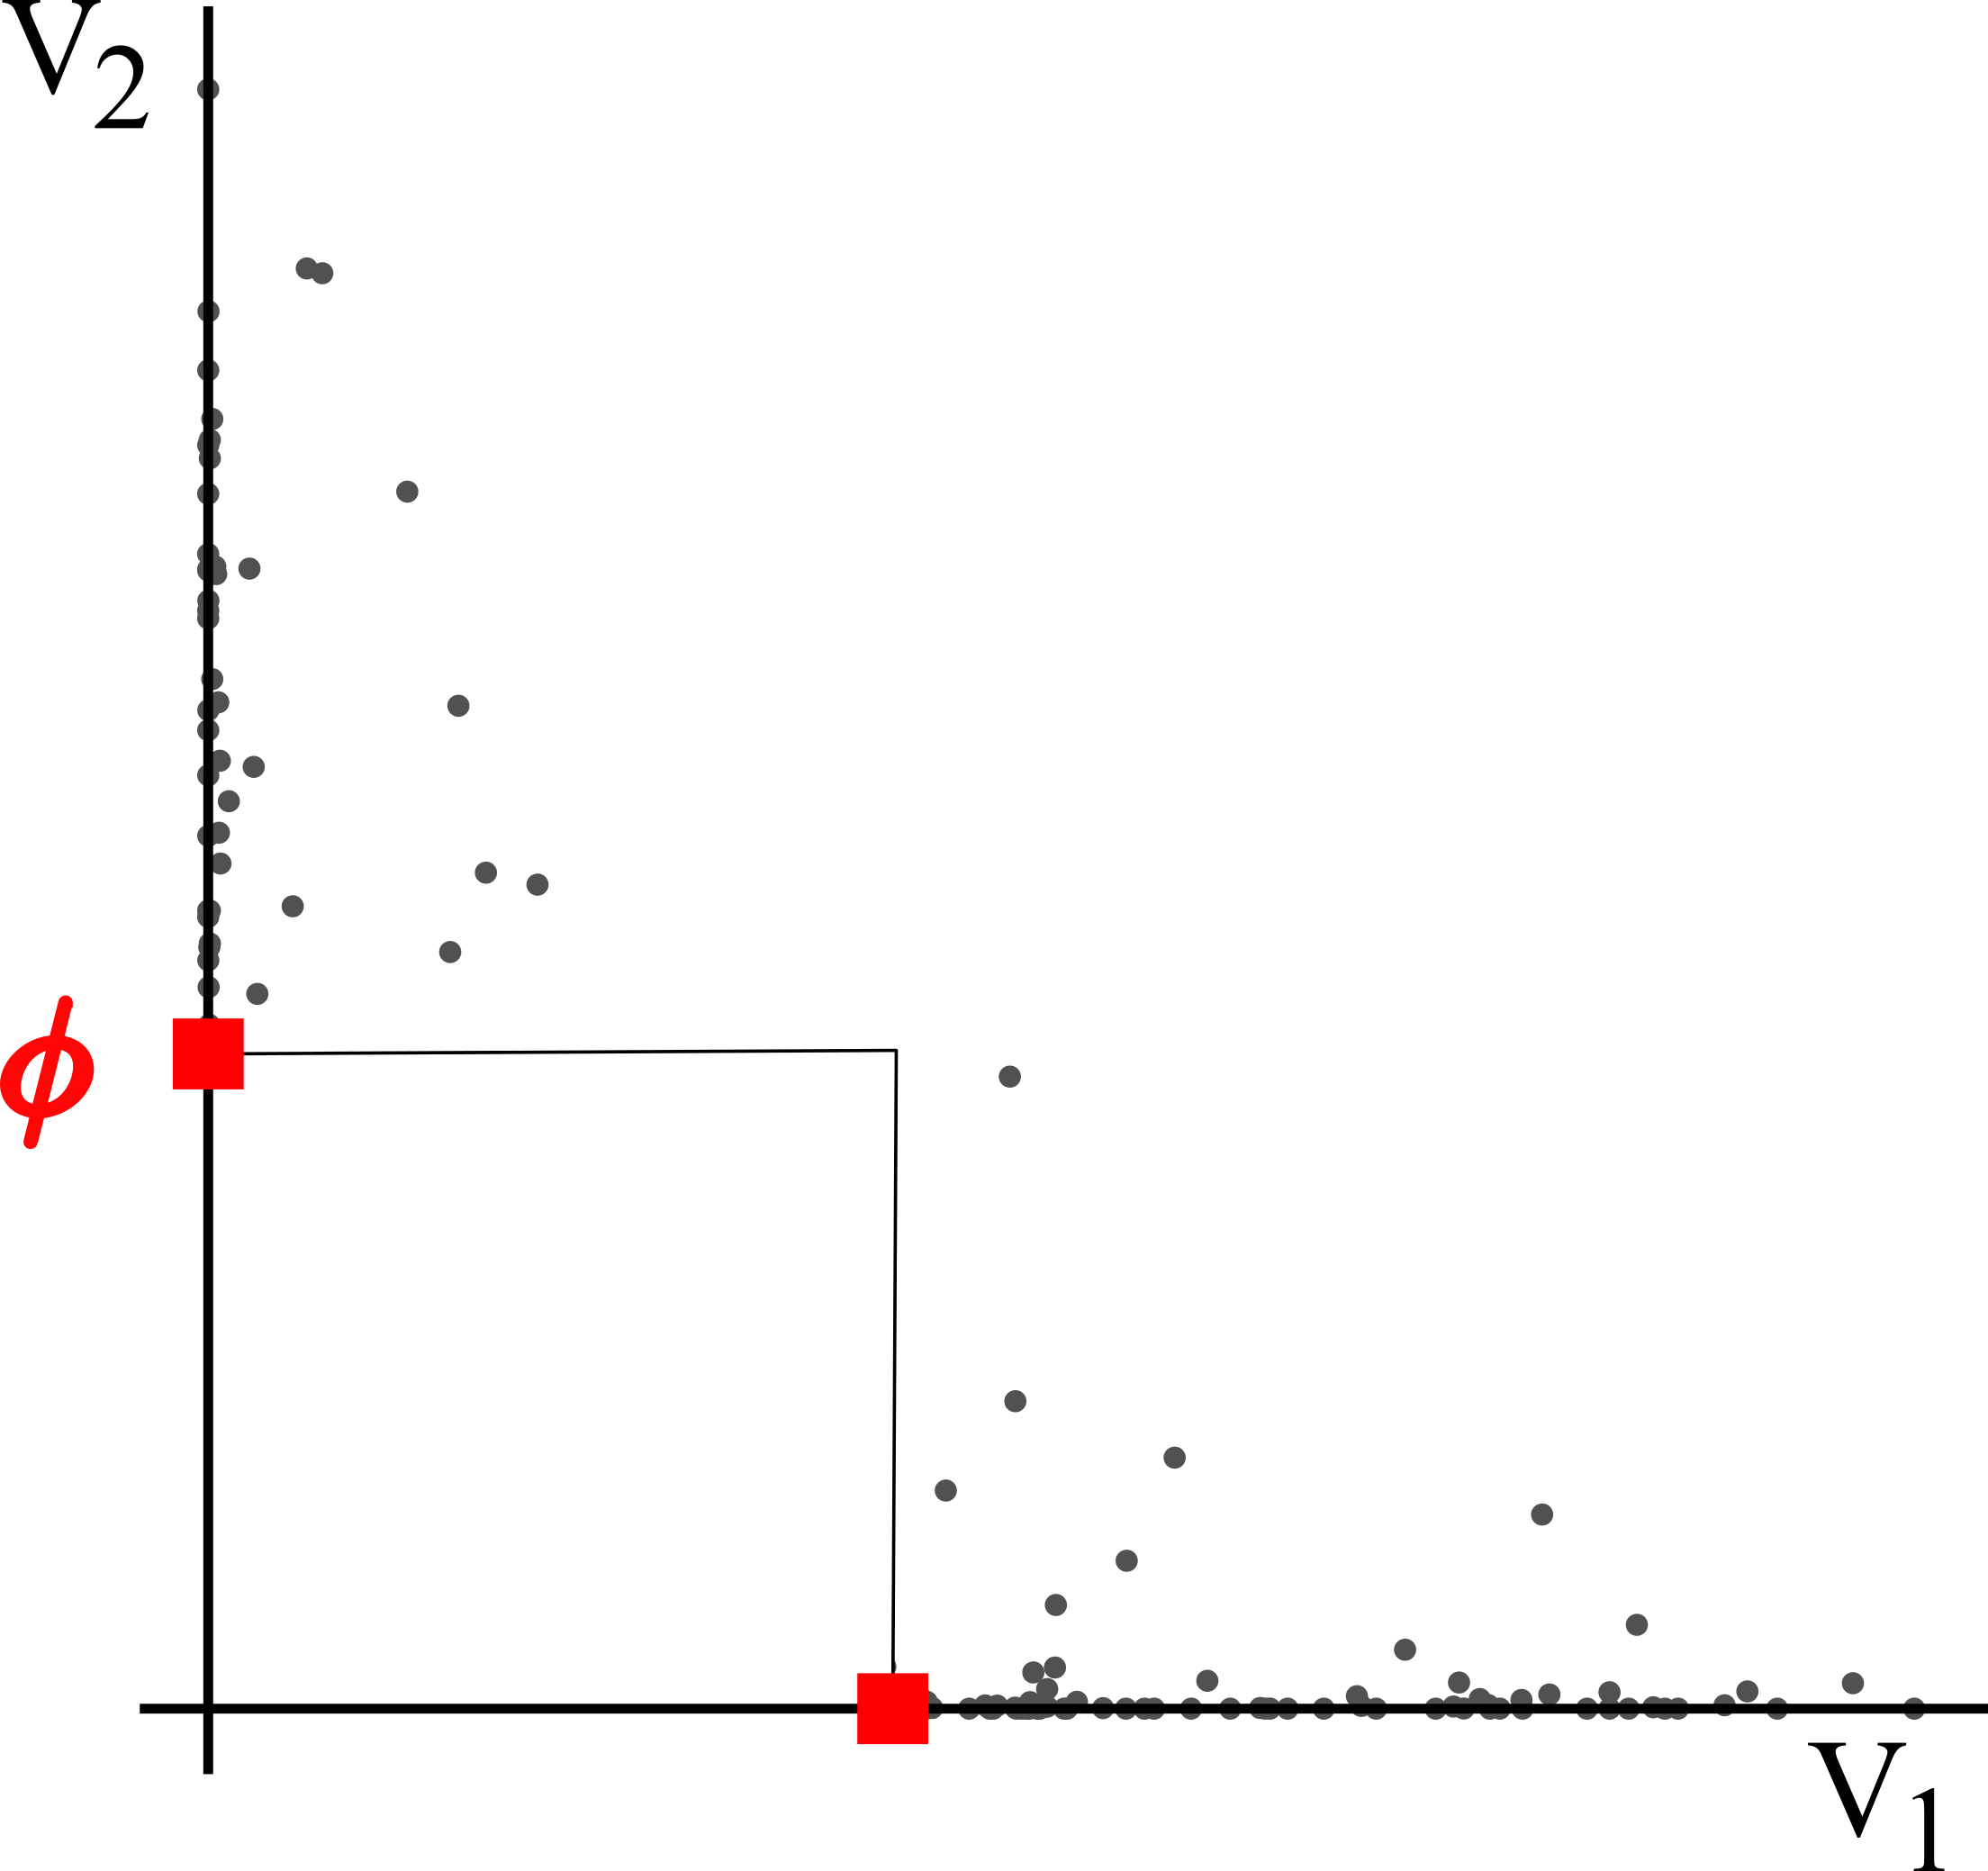
\includegraphics[scale=0.3]{sourcefigs/Example2D_indepSquare.png}
    \end{figure}

    \begin{tabular}{ll}
      Asymptotic dependence:  & ~~~~~~~~~~~~~~~~Asymptotic independence:\\
$(V_1,V_2)$ may be large together. & ~~~~~~~~~~~~~~~~Only $V_1$ \emph{or} $V_2$ may be large.
    \end{tabular}

\end{frame}


\begin{frame}
\frametitle{General Case}
  \begin{figure}
    \centering
    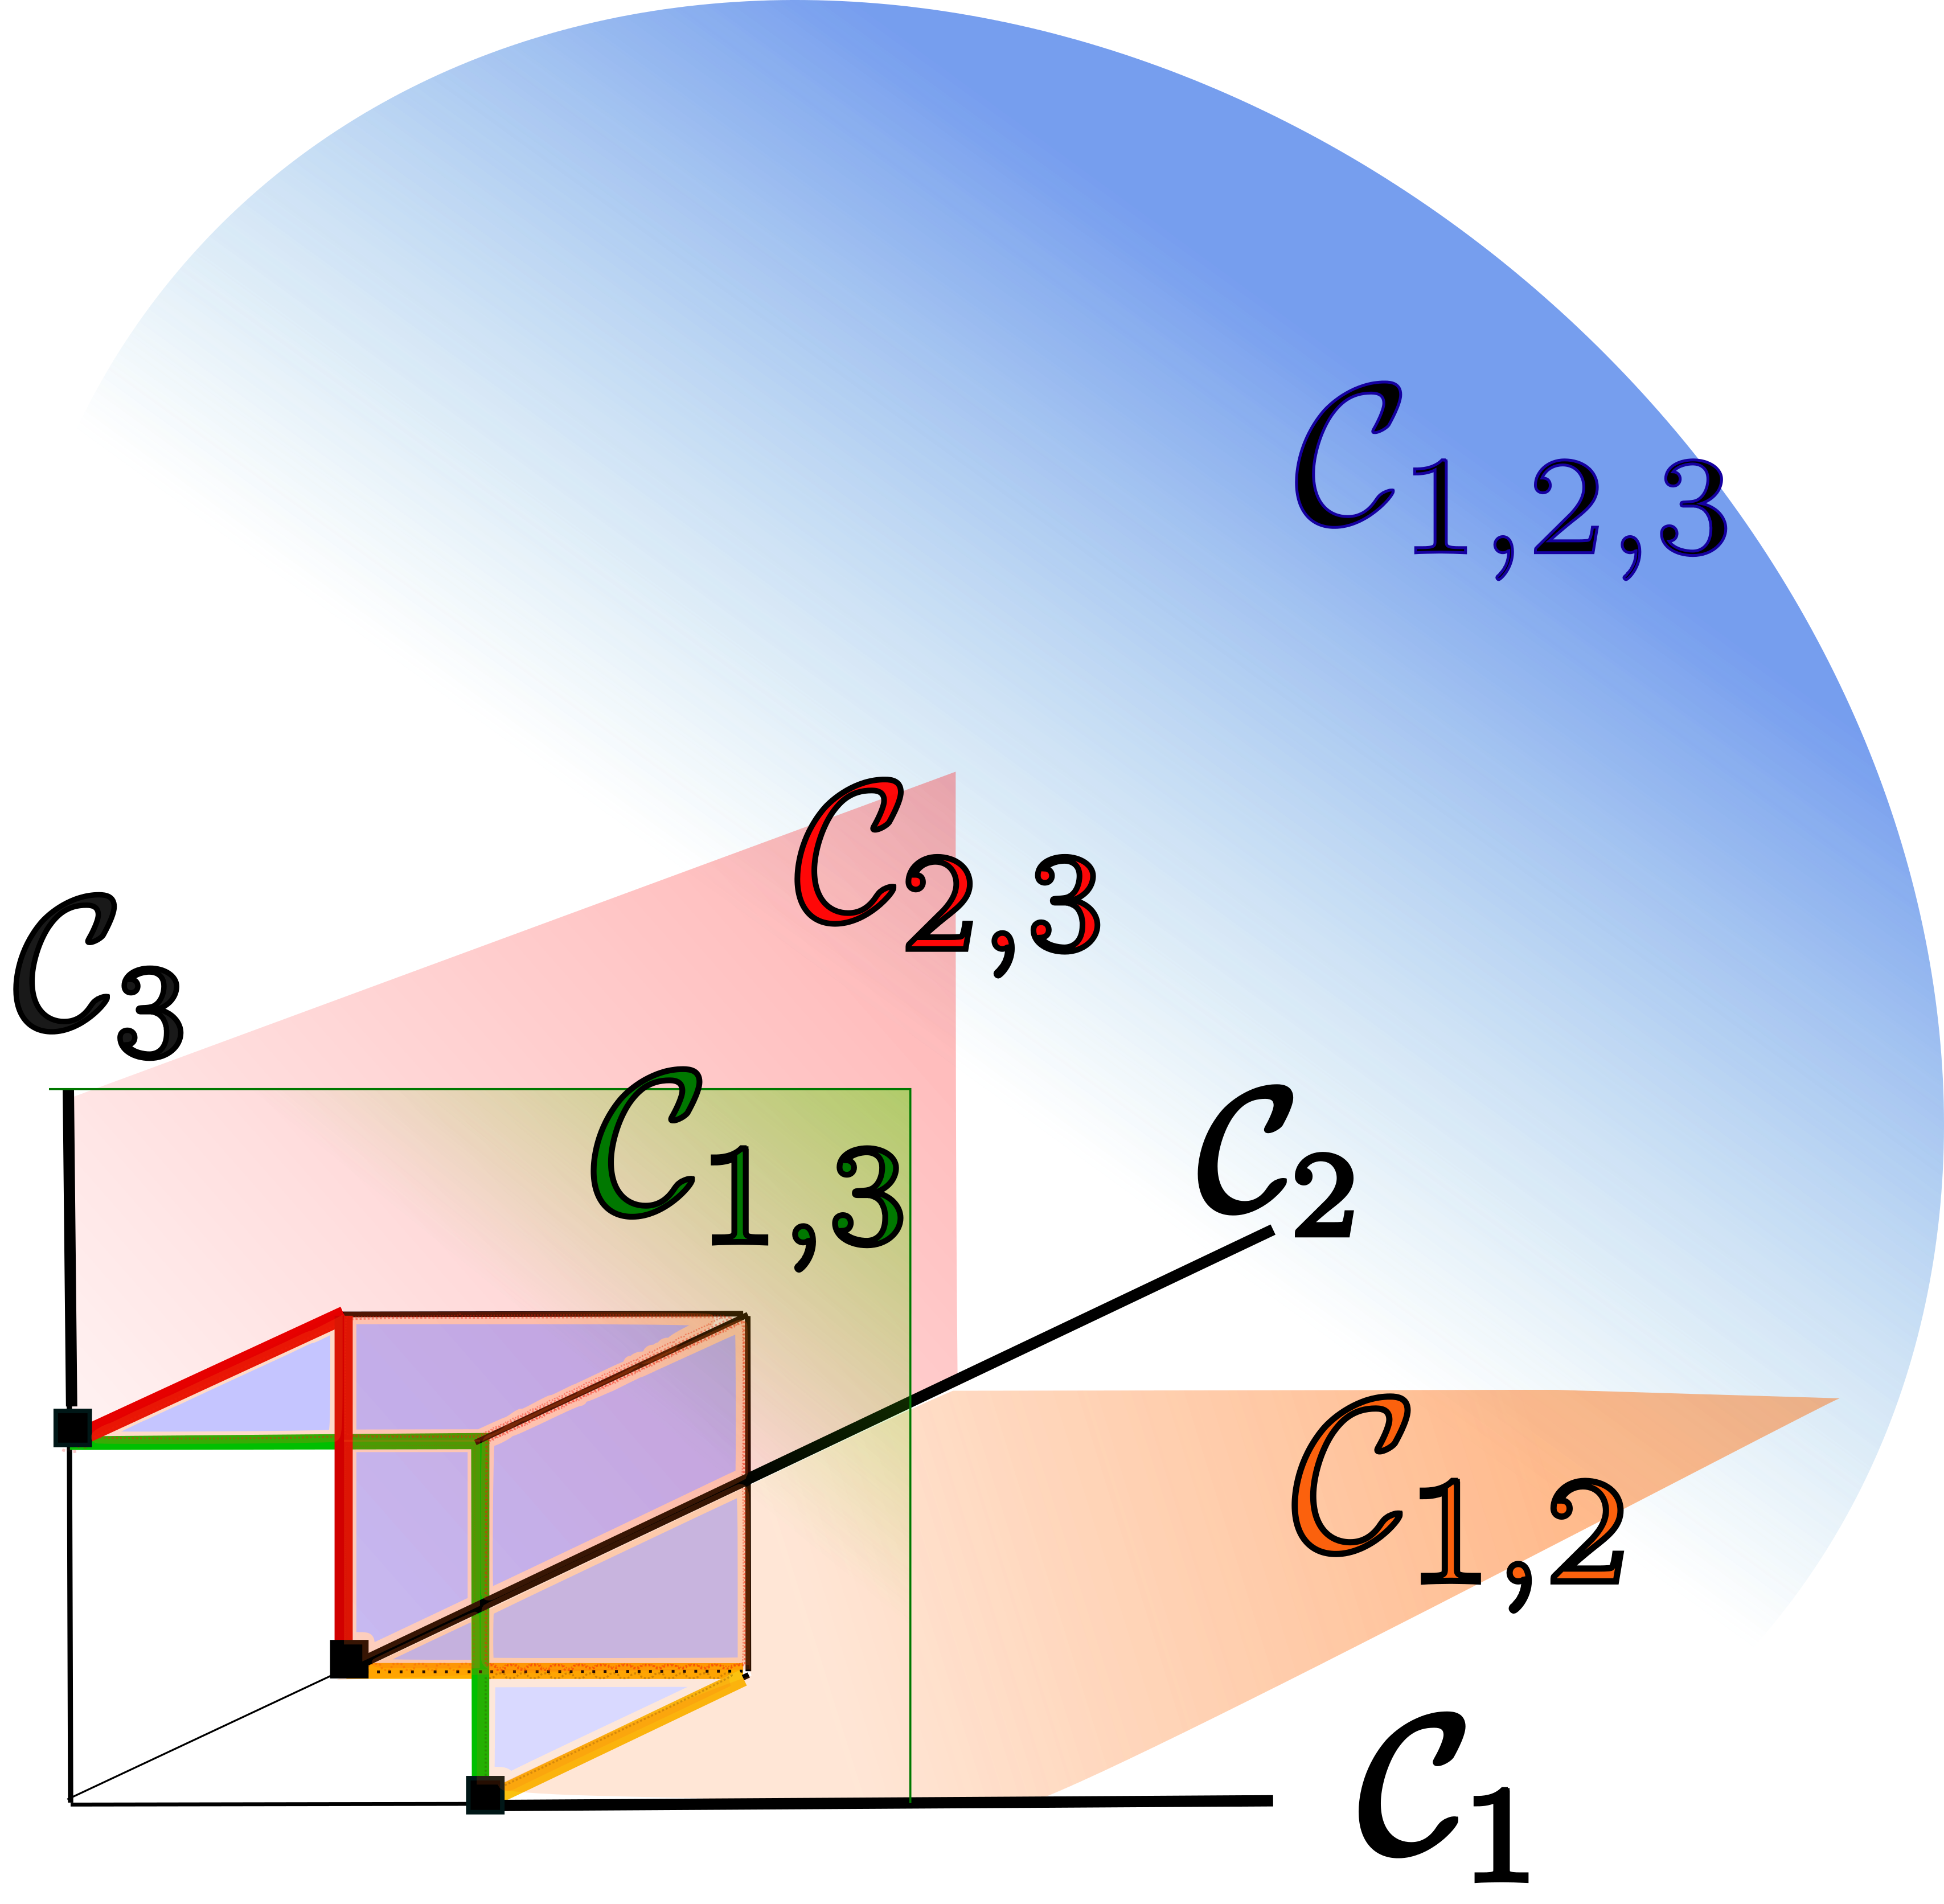
\includegraphics[width=0.4\linewidth]{sourcefigs/cone}
  \end{figure}
  \begin{itemize}
\item Sub-cones:  $\mathcal{C}_\alpha = \big\{\|v\|\ge 1,~~ v_j> 0 ~ (j\in\alpha),~~~  v_j = 0~(j\notin\alpha)\big\}$

\item   Corresponding sub-spheres: $\big\{\Omega_\alpha , \alpha\subset\{1,\dotsc,d\}\big\}$ ~~ ($\Omega_\alpha = \mathcal{C}_\alpha \cap \mathbf{S}_{d-1}$)
\end{itemize}
\end{frame}


% \begin{frame}
%   \frametitle{Joint extremes}
  
% \begin{figure}
% 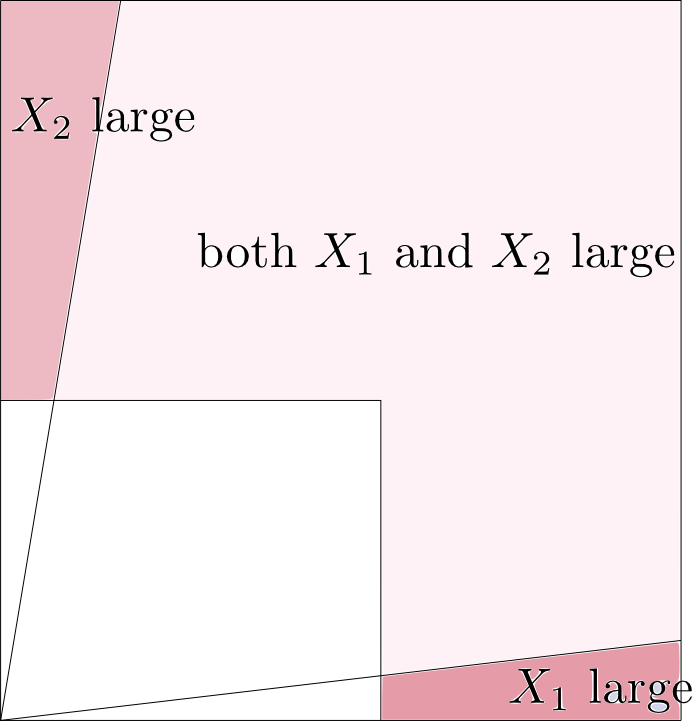
\includegraphics[width=0.68\linewidth]{sourcefigs/2DextremesIdea}
% \end{figure}
% \end{frame}


\begin{frame}
  \frametitle{Representation of extreme data}
\begin{itemize}
\item Natural decomposition of the angular measure :
$$
\Phi = \sum_{\alpha\subset\{1,\dotsc,d\}} \Phi_\alpha \text{~~~~~~~~~~~~~~~~~~with~~} \Phi_\alpha = \Phi_{|\Omega_\alpha} \leftrightarrow \mu_{|\mathcal{C}_\alpha}
$$


\item $\Rightarrow$ yields a representation
{\red
\begin{align*}
\mathcal{M} ~~&=~~ \Big\{~\Phi(\Omega_{\alpha}):~~~~ \emptyset \neq \alpha\subset\{1,\; \ldots,\; d \}~\Big\}  \\
&=~~ \Big\{~\mu(\mathcal{C}_{\alpha}):~~~~ \emptyset \neq \alpha\subset\{1,\; \ldots,\; d \}~\Big\}
\end{align*}
}  
% \begin{figure}
%     \centering
%     %\includegraphics[width=0.4\linewidth]{3D_anyH}\qquad 
%     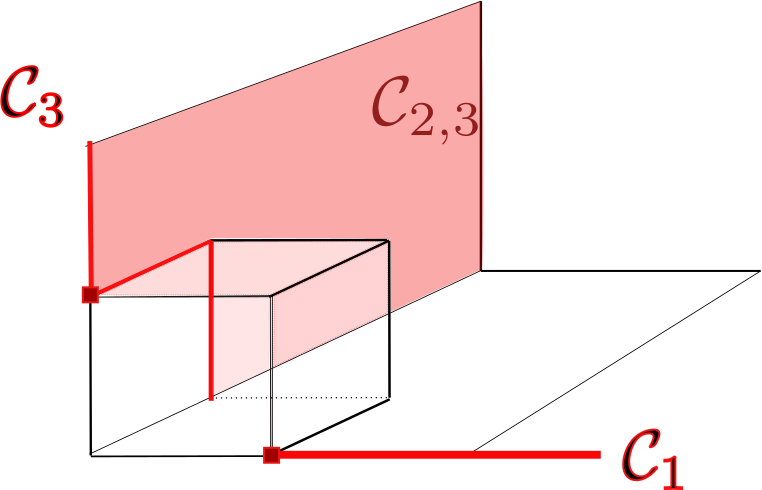
\includegraphics[width=0.3\linewidth]{sourcefigs/3D_sparseH}
%   \end{figure}

\item Assumption:  % $\Phi_\alpha = 0$ for $|\alpha|$ large,  and 
$\frac{\ud \mu_{|\mathcal{C}_\alpha}}{\ud v_\alpha} = O(1)$.\\~\\
 
%\item Remark: Representation $\mathcal{M}$ is linear (after non-linear transform of the data $\mb X \to \mb V$).
\end{itemize}


\end{frame}

\begin{frame}
\frametitle{Sparse Representation ?}
  \begin{figure}
    \centering
    \includegraphics[width=0.4\linewidth]{sourcefigs/3D_anyH}\qquad 
    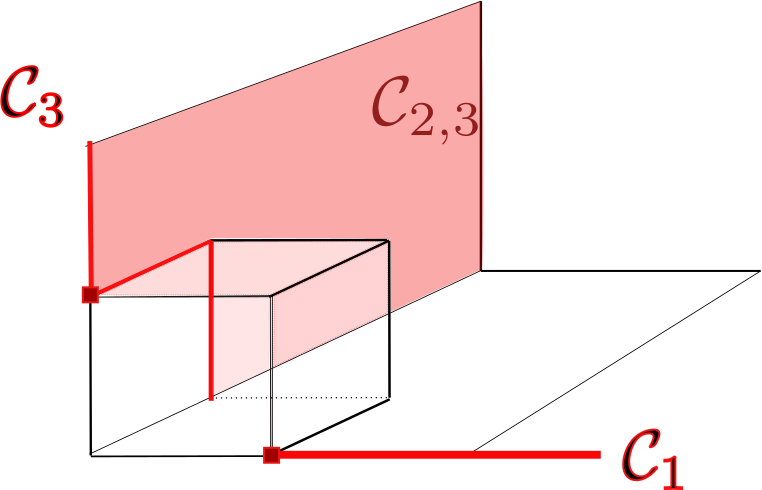
\includegraphics[width=0.4\linewidth]{sourcefigs/3D_sparseH} \\

 Full pattern : 
\hspace{3cm}   Sparse pattern  \\
{\footnotesize anything may happen}  \hspace{2cm} {\footnotesize ($V_1$ not large if
 $V_2$ or $V_3$ large)}
  \end{figure}
\end{frame}


% \subsection{Estimation}

\begin{frame}
\frametitle{Estimation}
\textbf{Estimation Problem}: $\mathcal{M}$ is an \textbf{asymptotic} representation
\begin{align*}
\mathcal{M} ~~=~~ \big\{~\Phi(\Omega_{\alpha}),~ \alpha~\big\} ~=~ \big\{~\mu(\mathcal{C}_{\alpha}),~ \alpha~\big\}
\end{align*}

is the restriction of an asymptotic measure 
\begin{align*}
\mu(A)=\lim_{t \to \infty} t \mathbb{P}[\mb V\in t~A]
\end{align*}
to a representative class of set $\{\mathcal{C}_\alpha,~\alpha\}$, but only the central sub-cone has positive Lebesgue measure!

\begin{minipage}{0.5\linewidth}
\centering
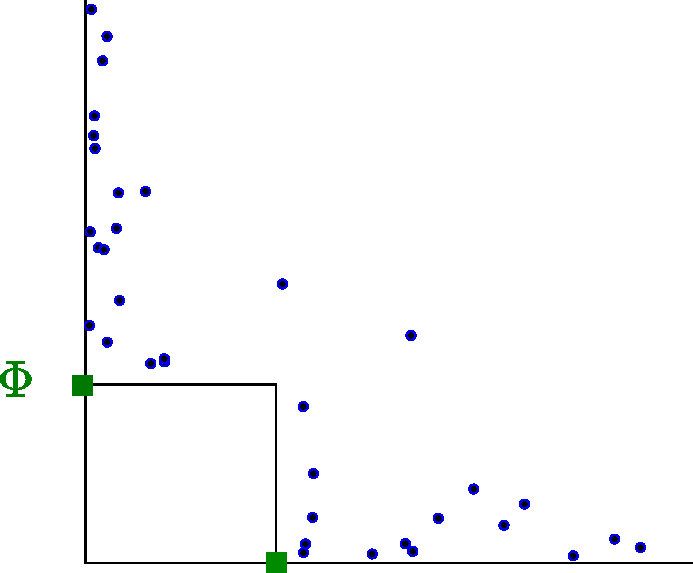
\includegraphics[scale=0.3]{sourcefigs/representation2D_problem.pdf}
\end{minipage}\hfill
\begin{minipage}{0.5\linewidth}
$\Rightarrow$ Cannot just do, for large $t$:
\begin{align*}
\Phi(\Omega_\alpha) = \mu(\mathcal{C}_\alpha) \simeq t \widehat{\mathbb{P}}(t \mathcal{C}_\alpha)
\end{align*}
\end{minipage}

\end{frame}

\begin{frame}
\frametitle{Solution}
 \textbf{Fix $\epsilon>0$. Affect data  $\epsilon$-close to an edge,
   to that edge. }

\begin{figure}[h]
  \centering
  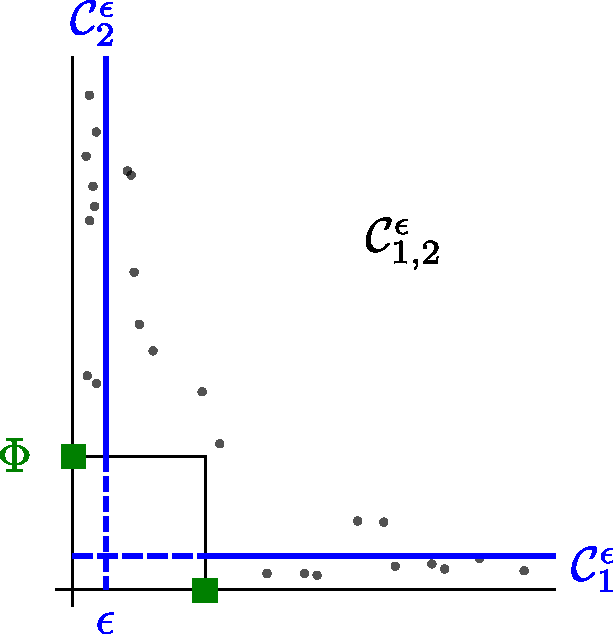
\includegraphics[scale=0.4]{sourcefigs/representation2Drect.pdf}
\end{figure}

\begin{align*}
\mathcal{C}_\alpha\to \mathcal{C}_\alpha^\epsilon &= \{\|v\|\ge 1,~~ v_j>\epsilon\, (j\in\alpha),\,v_j \le \epsilon \,(j\notin\alpha) \}. 
%\Omega_\alpha  \to  \Omega_\alpha^\epsilon&= \mathcal{C}_\alpha^\epsilon \cap \mathbf{S}_{d-1}
\end{align*}
New partition. %of $\mathbf{S}_{d-1}$.%, compatible with non asymptotic data.
\end{frame}


\begin{frame}
\frametitle{Resulting estimation procedure}
$\hat V_i^j = \frac{1}{1- \hat F_j(X_{i}^j)}$ with 
$\hat F_j(X_{i}^j) =\frac{rank(X_i^j) -1}{n} $\\~\\~\\

\begin{minipage}{0.5\linewidth}
%\centering
Recall that:
\begin{align*}
\mu(A)=\lim_{t \to \infty} t \mathbb{P}[\mb V\in t~A]
\end{align*}
%
$\Rightarrow$ get an natural estimate of $\Phi(\Omega_\alpha)$
\begin{align*}
&\widehat{\Phi}(\Omega_\alpha) := \frac{n}{k}\mathbb{P}_n( \hat V \in \frac{n}{k}\mathcal{C}_\alpha^\epsilon)\\
&(\frac{n}{k}~~ \text{large}, ~\epsilon~~ \text{small})
\end{align*}
\end{minipage}\hfill
\begin{minipage}{0.5\linewidth}
\centering
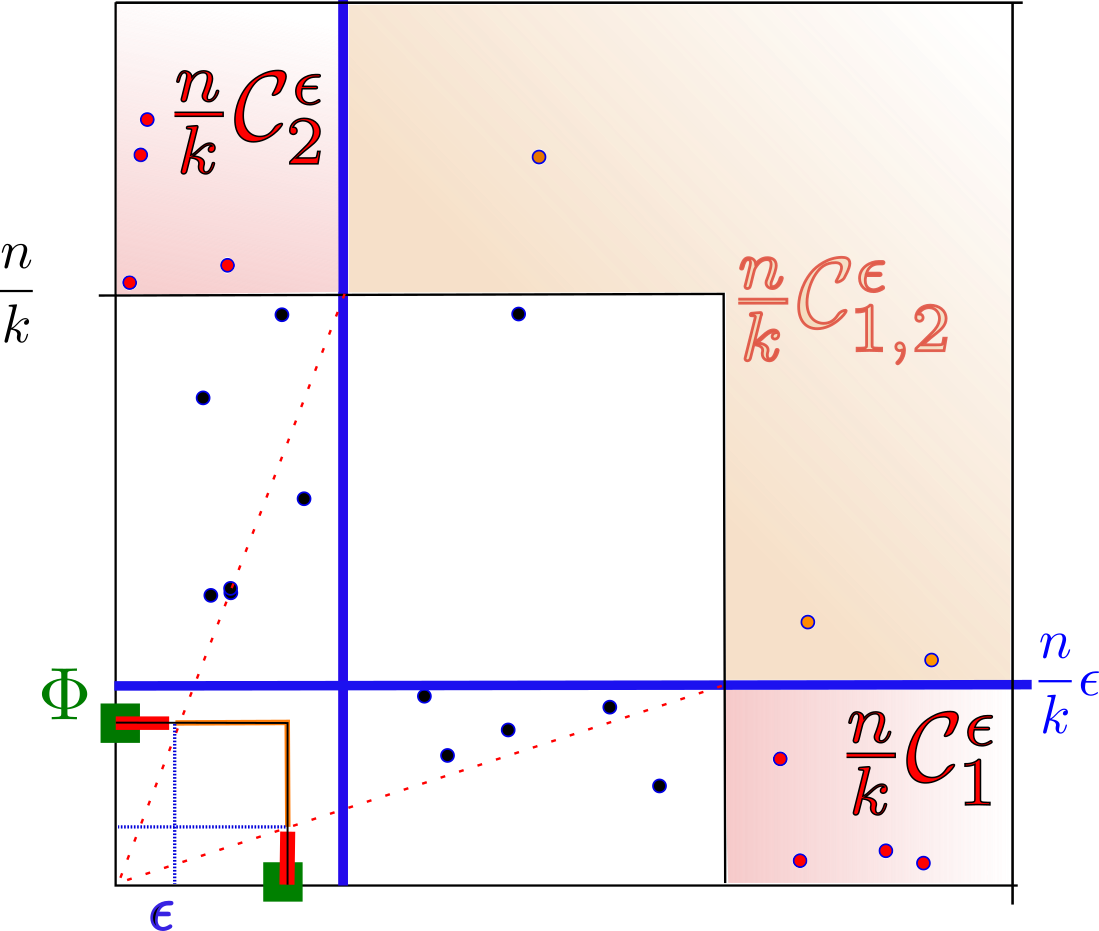
\includegraphics[scale=0.45]{sourcefigs/representation2D_nk_rect.png}
\end{minipage}
~\\~\\~\\
$\Rightarrow$ we obtain
$$\widehat{\mathcal{M}}:=\big\{~\widehat{\Phi}(\Omega_{\alpha}),~ \alpha~\big\}$$
\end{frame}





\begin{frame}
\frametitle{Statistical guaranties}

\begin{block}{Theorem {\small [Goix, Sabourin, Clémençon 2016]}}
There is an absolute constant $C > 0$ such that for any $n>0,~ k>0,~ 0<\epsilon<1,~ \delta>0$ such that $0<\delta<e^{-k}$, with probability at least $1 - \delta$,
\begin{align*}
\|\widehat{\mathcal{M}}- \mathcal{M}\|_\infty
~\le~  C d \left( \sqrt{ \frac{1}{\epsilon k}\log\frac{d}{\delta}} + M d\epsilon \right) + \text{bias}(\epsilon, k, n)
\end{align*}
\end{block}
~\\
\textbf{Comments:}
% % \[
% % \begin{aligned}
% $
% \text{error}%\hat \Phi_n(\Omega_\alpha) - \Phi(\Omega_\alpha^0)|
% % |\mu_n(\mathcal{C}_\alpha^\epsilon) - \mu(\mathcal{C}_\alpha^0)|
% ~\le~  \Big( {\color{blue}\frac{C  d}{k^{1/4}} \sqrt{
%     \log\frac{d}{\delta}}} ~+~ %\
% {\color{violet}~ 5\sup_{0 \le x \le \frac{2 \sqrt k}{d}}\big|\frac{n}{k} \tilde F(\frac{k}{n}x)-\frac{n}{k} l ( \frac{k}{n} x)\big| }\Big)  
% $~\\~\\~\\
%
% $\Big(${\color{blue} variance $O(1/k^{1/4})$} + 
% {\color{violet} bias  }$\Big)$
\begin{itemize}


\item $M \simeq \sum_\alpha \sup$(density on cones $\alpha$)


\item  Existing literature (for spectral measure) {\small [Einmahl and Segers 09, Einmahl \emph{et al.} 01]}

  \begin{center}
$d=2$, asymptotic behavior, rates  in $1/\sqrt k$.
  \end{center}
\item Here: $1/\sqrt k\to  1/\sqrt{\epsilon k} + \epsilon$. Price to pay
for biasing our estimator with $\epsilon$.
\end{itemize} 
\end{frame}




\begin{frame}
\frametitle{Theorem's proof: key ingredient}
% \frametitle{Statistical guarantees: Main issue}
Would like to use concentration inequality... % XXX citer boucheron?
% XXX 2 dessins
\begin{align*}
&\text{In our case:~~~~~~} \sup_{A \in \mathcal{A}} {\red\frac{n}{k}}\left| \big(\mathcal{P}- \mathcal{P}_n\big)\left({\blue \frac{n}{k}}A\right)\right|\\
&\text{But usually:~~~~~~~~~~~~} \sup_{A \in \mathcal{A}} \left| \big(\mathcal{P}-\mathcal{P}_n\big)(A) \right|
\end{align*}
\begin{itemize}
\item scaling ${\red \frac{n}{k}}$%: to compense the decreasing proba of ${\blue \frac{k}{n}}A$.\\
\item classical VC-inequality: ${\blue \frac{n}{k}}$ nice but not used ! \\$\rightarrow $ high proba bound in $${\red \frac{n}{k}} \times  \sqrt{ \frac{1}{ n}\log \frac{1}{\delta}} ~~~~~~\to~~ ~~\infty~~~~ !! $$ \\
\end{itemize}

$\Rightarrow$ Needs to take into account that the proba of  ${\blue \frac{n}{k}}A$ is small.\\
\end{frame}


\begin{frame}
\frametitle{Theorem's proof: key ingredient}
% \frametitle{Statistical guaranties: Solution}
\textbf{Key:}
VC-inequality adapted to rare regions $\rightarrow$ bound in $$\mathbf{{\blue \sqrt{p}}}~ {\red \frac{n}{k}} \sqrt{ \frac{d}{ n}\log \frac{1}{\delta}}$$
with $p$ the probability to be in the union class $\cup_{A \in \mathcal{A}}A$.
$$\mb {\blue p} \le d \frac{k}{n}$$
$\Rightarrow$ bound in $$ d \sqrt{ \frac{1}{ k}\log \frac{1}{\delta}} $$
%interpretation of $k$: 
%\begin{itemize}
%\item 
~\\
$k \propto$ number of data considered as extreme (data used for estimation)
%\item $k \simeq$ number of data 
%\end{itemize}

\end{frame}


% \begin{frame}
% \frametitle{Theorem's proof}
% % \begin{enumerate}
% % \item \textbf{Maximal deviation on VC-class:}
% %  \only<1>{ 
% % %Bound on the maximal deviation of $\mu_n$ on simple VC-class:
% % $$
% % \sup_{x\succeq {\epsilon}} |\mu_n - \mu| ([x,\infty[)  \le
% % {\color{blue} Cd\sqrt{\frac{2}{k}\log\frac{d}{\delta}} }  +
% %   {\color{violet} \text{bias}(\epsilon, k, n)% \text{bias}_{ \,\tilde F \leftrightarrow l, x\le 1/\epsilon}
% %   }
% % $$
% % \textbf{Tools}: Vapnik-Chervonenkis inequality adapted to small probability sets: bounds in ${\color{red}\sqrt{p}}\sqrt{\frac{1}{n}\log\frac{1}{\delta}}$.\\~\\

% % On the VC class $\{ [\frac{n}{k} x, \infty]$, $x \ge \epsilon \}$.

% % %   \begin{itemize}
% % %   \item 
% % %     \begin{itemize}
% % %     \item 
% % %    \item with nearly uniform
% % %     data $\hat U_{i,j} = 1 - \hat F_j(Y_{i,j}) ~( = 1/\hat X_{i,j})$.
% % %     \end{itemize}
% % % % $\exists C, \text{ indep from } n, d$, s.t., with proba $1-\delta$,
% % % \end{itemize}
% % }
% % \only<2>{~\\~\\ \item
%   \textbf{Decompose error:}
%   \[|\mu_n(\mathcal{C}_\alpha^\epsilon) - \mu(\mathcal{C}_\alpha)| \le 
% \underbrace{|\mu_n- \mu|(\mathcal{C}_\alpha^\epsilon)}_A +
% \underbrace{ |\mu(\mathcal{C}_{\alpha}^\epsilon) - \mu(\mathcal{C}_\alpha) |}_B \]\\
% \begin{itemize}
% % \item 
%  % Restriction to cube $[0,L]$, 
% \item term $A : $ Bounded with VC inequality adapted to small probability regions.\\~\\
% \item % $B  = O( M d^2 (\epsilon )^{d-\alpha}) $ $\to $ OK with boundedness
%   % assumption.
%   term $B  :$ $\text{Leb}(\mathcal{C}_{\alpha}^\epsilon \setminus \mathcal{C}_{\alpha})$ is small when $\epsilon$ is small.\\~\\%% O( M (d^2 \epsilon + (1+\epsilon)^d -1)) $ % $\to $ OK with boundedness
%    % assumption.

% % %% $A=O\Big(~ 2^\alpha  E  + M \alpha d (\epsilon L)  + Md^2
% %                                  (1+ \epsilon L )^{d}-1   
% % +
% %   \frac{1}{L}~\Big)$ \\

% %\item Optimize in $L, \epsilon \Rightarrow \epsilon=d/\sqrt k$  \\
% %explains the $k^{1/4}$ loss compared with low dimension.

% \end{itemize}
% % }
% % \end{enumerate}
% \end{frame}




\begin{frame}
\frametitle{Application to Anomaly Detection}

Recall that after standardization of marginals: 
$\mathbb{P}[R> r  ,\mb W \in B ]  \simeq \frac{1}{r}\,\Phi(B)$ \\~\\
 $\rightarrow$ scoring function = $\Phi_n^\epsilon$  $\times 1/r:$
$$s_n(\mb x):= (1/\|\hat T(\mb x)\|_\infty) \sum_{\alpha }\Phi_n^{\alpha, \epsilon} \mathds{1}_{\hat T(\mb x) \in \mathcal{C}_\alpha^\epsilon}.$$
 where $\hat T: \mb X \mapsto \mb V$ ~~~~~~~~~($\hat V_{j} = \frac{1}{1- \hat F_j (X_{j})} $)

  \begin{figure}
    \centering
    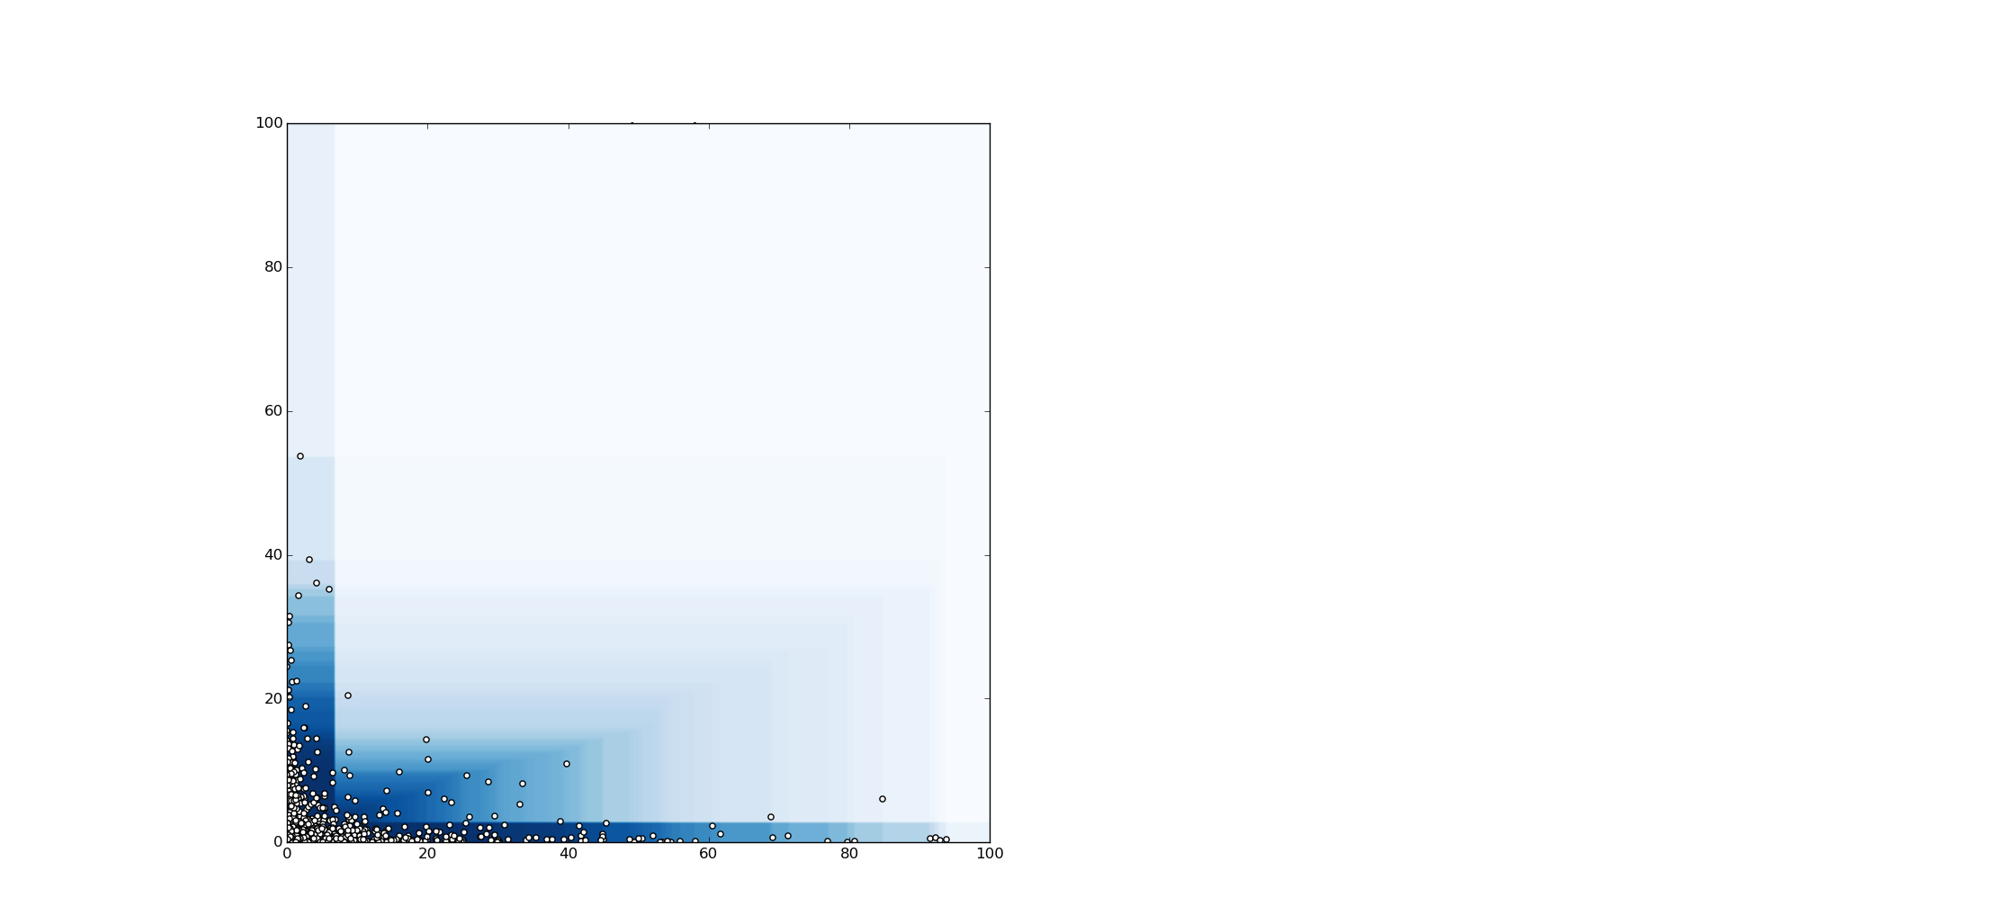
\includegraphics[scale=0.206, trim=2cm 0cm 2cm 1cm]{sourcefigs/plot_damex_level_sets}
  \end{figure}

\end{frame}


\section{Part III: Heuristic contributions and perspectives}

% \subsection{Evaluation of scoring functions, model selection}

\begin{frame}
\frametitle{EM and MV curves for model selection?}

%\subsection{Goal of Anomaly Detection }
%Anomaly: "an observation which deviates so much from other observations as to arouse suspicions that it was generated by a different mechanism (Hawkins 1980)"

% MV and EM curves allow to build scoring functions.

% \textbf{Question:} Can we use them for evaluating any scoring function?


\begin{block}{Practical motivations:}
Most of the time, data come without any label.\\
{\footnotesize ~~~~~~ $\to$ no ROC or PR curves!}
\end{block}
~\\~\\
% \begin{block}{Implicit (natural) simplification of the problem:}
% How good is an anomaly detection algorithm?\\
% $\to$ How good is it estimating the level sets of the inliers distribution?
% \end{block}

% Inputs: scoring function $s$
\textbf{Estimation:}
{\small
\begin{align*}
&\widehat{MV}_s(\alpha) = \inf_{u \ge 0} ~~~\leb(s \ge u) ~~~~\st~~~~ \mathbb{P}_n(s \ge u) \ge \alpha\\% ~~~~~~~~\to \widehat{\crit}^{EM}(s) = \|\widehat{MV}_s\|_{1, J}\\
&\widehat{EM}_s(t) = \sup_{u \ge 0} ~~~\mathbb{P}_n(s \ge u) ~-~ t \leb(s \ge u)% ~~~~~~~~~~~~~~~~~~~~~\to \widehat{\crit}^{MV}(s) = \|\widehat{EM}_s\|_{1, I}
\end{align*}
}
~\\~\\
{\small [Thomas et al. 2015]}\\

% \item \textbf{Empirical criteria:}
% \small{
% \begin{align*}
% \widehat{\crit}^{EM}(s) &= \| \widehat{EM}_s \|_{L^1(I)}  &&I = [0,\widehat{EM}^{-1}(0.9)],\\
% \widehat{\crit}^{MV}(s) &= \| \widehat{MV}_s \|_{L^1(J)}  &&J = [0.9, 1],
% \end{align*}
% }
~\\
\textbf{Issue in large dimensions:}\\
The volume $\leb(s \ge u)$ has to be estimated! % Challenging in high dimensions.

\end{frame}


\begin{frame}
\frametitle{EM and MV curves for model selection?}

\textbf{Heuristic extension for large dimension:}

\begin{block}{Random projection and averaging ~~~~{\color{black} \small [Goix 2016]}}~\\

\small{
%\begin{algorithm}
\begin{algorithmic}

  \STATE \textbf{Inputs}: AD algorithm $\mathcal{A}$, data set $X$ size $n \times d $, feature sub-sampling size $d'$, number of draws $m$.\\~\\
  \FOR{$k=1,\ldots,m$}
    \STATE{-randomly select a sub-group $F_k$ of $d'$ features}
    \STATE{-compute the associated scoring function $s_{k} = \mathcal{A}\big((x^j_i)_{1 \le i \le n,~j \in F_k}\big)$}
    \STATE -compute $\widehat{\crit}_k^{EM} = \| \widehat{EM}_{s_k} \|_{L^1(I)}$  or $\widehat{\crit}_k^{MV} = \| \widehat{MV}_{s_k} \|_{L^1(J)}$
  \ENDFOR \\~\\

  \STATE \textbf{Return} performance criteria: $$\widehat{\crit}^{EM}_{high\_dim} (\mathcal{A})= \frac{1}{m} \sum_{k=1}^m\widehat \crit_k^{EM} \text{~~~~or~~~~} \widehat{\crit}^{MV}_{high\_dim}(\mathcal{A}) = \frac{1}{m} \sum_{k=1}^m\widehat \crit_k^{MV}~.$$

\end{algorithmic}
%\end{algorithm}
}
\end{block}
Seems to work in practice but no statistical guaranties.
\end{frame}

% \subsection{One-class splitting criterion for random forests}

\begin{frame}
\frametitle{Random Forests for one-class classification}

% {\blue Two-class impurity decrease} (proxy) for splitting node $t$, yielding children nodes $t_L$ and $t_R$ :

\begin{block}{Two-class Random Forests [Breiman, 2001]}
\begin{minipage}{0.65\textwidth}
\textbf {Two-Class impurity decrease} 
\begin{align*}
I_G(t_L, t_R)= \frac{{\blue n_{t_L}} {\red n'_{t_L}}}{{\blue n_{t_L}} +  {\red n'_{t_L}}} + \frac{{\blue n_{t_R}} {\red n'_{t_R}}}{{\blue n_{t_R}} +  {\red n'_{t_R}}}.
\end{align*}
$n_t$ : nb of observations with label $0$ in node $t$.\\
$n_t'$: nb of observations with label $1$ in node $t$.

\end{minipage}
\begin{minipage}{0.3\textwidth}
	\centering
	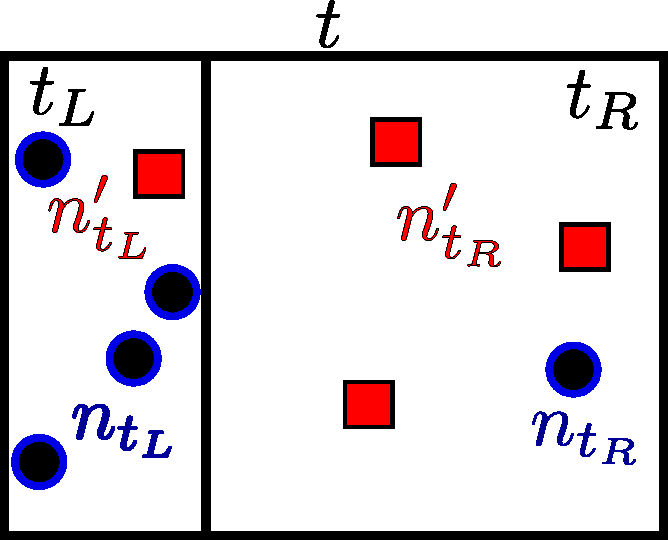
\includegraphics[width=0.95\textwidth]{sourcefigs/tree.pdf}
\end{minipage}
\end{block}
~\\~\\

\begin{exampleblock}{Random Forests for one-class classification}
\begin{minipage}{0.65\textwidth}
\begin{align*}
&\text{Two-Class:}~~~
I_G(t_L, t_R)= \frac{{\blue n_{t_L}} {\red n'_{t_L}}}{{\blue n_{t_L}} +  {\red n'_{t_L}}} + \frac{{\blue n_{t_R}} {\red n'_{t_R}}}{{\blue n_{t_R}} +  {\red n'_{t_R}}}.\\
&\text{One-Class:}~~~ {\red n'_{t_L}},~ {\red n'_{t_R}} = \text{?}
\end{align*}

\end{minipage}
\begin{minipage}{0.3\textwidth}
	\centering
	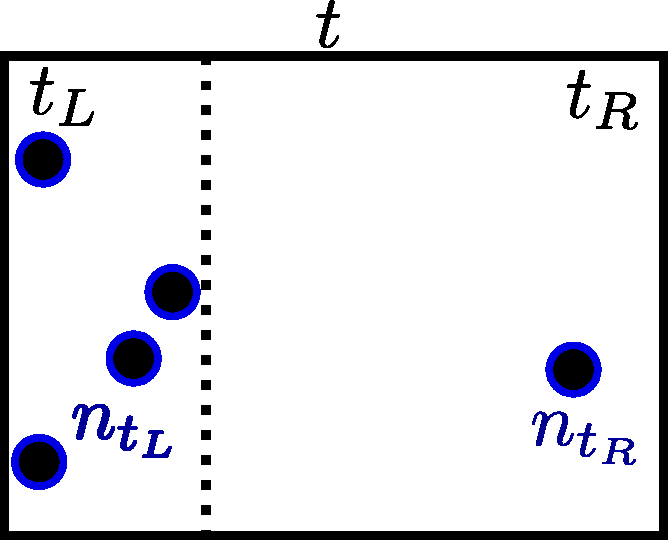
\includegraphics[width=0.95\textwidth]{sourcefigs/tree_oc.pdf}
\end{minipage}

Existing literature:
{\small [Liu et al., 2008, Désir et al., 2013, Shi and Horvath, 2012].}\\
Based on \textbf{second-class sampling}.
\end{exampleblock}
\end{frame}



\begin{frame}
\frametitle{Random Forests for one-class classification}

% {\blue Two-class impurity decrease} (proxy) for splitting node $t$, yielding children nodes $t_L$ and $t_R$ :

\begin{minipage}{0.65\textwidth}
\begin{align*}
&\text{Two-Class:}~~~
I_G(t_L, t_R)= \frac{{\blue n_{t_L}} {\red n'_{t_L}}}{{\blue n_{t_L}} +  {\red n'_{t_L}}} + \frac{{\blue n_{t_R}} {\red n'_{t_R}}}{{\blue n_{t_R}} +  {\red n'_{t_R}}}.\\
&\text{One-Class:}~~~ {\red n'_{t_L}},~ {\red n'_{t_R}} = \text{?}
\end{align*}

\end{minipage}
\begin{minipage}{0.3\textwidth}
	\centering
	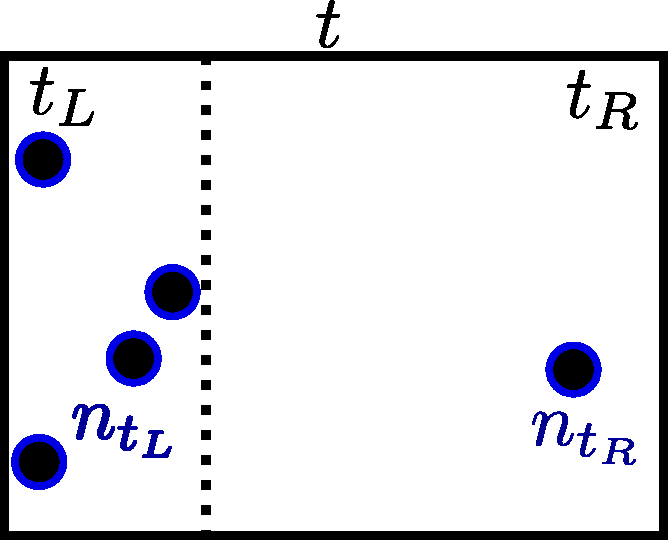
\includegraphics[width=0.95\textwidth]{sourcefigs/tree_oc.pdf}
\end{minipage}
\
\begin{exampleblock}{One-Class splitting criterion ~~~~{\color{black} \small [Goix, Brault, Drougard, Chiapino 2016]:}}
\textbf{Naive approach:} ~~~~~~~~~${\red n'_{t_L}} \to {\mb n} \frac{\leb(t_L)}{\leb(\mb{t_{0}})} ~~~~\text{and}~~~~ {\red n'_{t_R}} \to \mb n \frac{\leb(t_R)}{\leb(\mb{t_{0}})}$~~~~~~~($\mb{t_0}$ root node)

\textbf{Adaptive approach:}~~~
${\red n'_{t_L}} \to \mb{n_{t}} \frac{\leb(t_L)}{\leb(\mb t)} ~~~~\text{and}~~~~
{\red n'_{t_R}} \to \mb{n_{t}} \frac{\leb(t_R)}{\leb(\mb t)}
$
% \begin{align*}
% I_G^{OC-ad}(t_L, t_R)= \frac{{\blue n_{t_L}} \gamma n_t \lambda_L}{{\blue n_{t_L}} + \gamma n_t \lambda_L} + \frac{{\blue n_{t_R}} \gamma n_t \lambda_R}{{\blue n_{t_R}} + \gamma n_t \lambda_R}.
% \end{align*}

\begin{figure}[!ht]
  \centering
\resizebox{1.01\linewidth}{!} {
  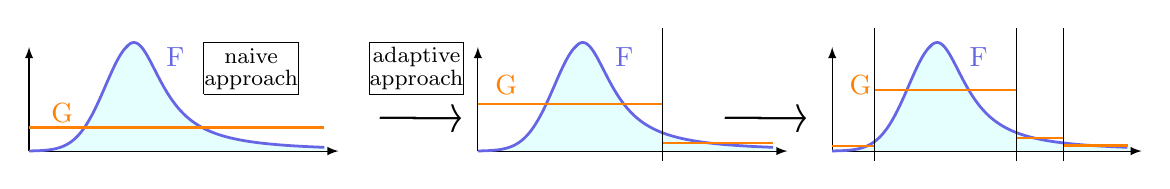
\begin{tikzpicture}[scale=0.6,declare function={
    %%cauchy distrib
    c1 = 6/10;
    c2 = 4/10;
    seuil = c1/(c1+c2);
    a1 = 0.1;
    a2 = 0.2;
    x01 = 0.8;
    x02 = 2.9;
    cauchyMass1(\x) = c1*a1/( pi*( pow(a1,2) + pow((\x-x01),2) ));
    cauchyMass2(\x) = c2*a2/( pi*( pow(a2,2) + pow((\x-x02),2) ));
    loinormale(\x) = c2*exp(-pow((\x-x02),2)/0.05);
    loinormale2(\x) = c2*exp(-pow((\x-x02-1.5),2)/0.3);
      indicatorFunction(\x) = exp(-pow(\x-3,2)/6);
      %%params
      firstVerticalSplitX = 1;
      lastVerticalSplitX = 5.7;
      verticalDashedSplitX = 2.3;
      verticalSplitX = 4;
      lowHorizontalDashedSplitY = 4.5;
      highHorizontalDashedSplitY = 5.5;
      coeffHomothety = 3.8;
      homothetyBone = -1.7;
      homothetyBtwo = -14;
    },
]
  \definecolor{niceblue}{rgb}{0.4,0.4,0.9}
    \definecolor{blue2}{rgb}{0.9,1,1}
\definecolor{ggreen}{rgb}{0.3,0.7,0.4}
\definecolor{orange2}{rgb}{1,0.7,0}

%%%%%%%%%%%%%%%% FIRST curve

\fill [blue2, domain=-7.9:-1.65, variable=\x]
      (-7.9, 1)
      -- plot[samples=200,smooth] ({\x},{ 1.5*coeffHomothety*loinormale((\x-homothetyBone+15)/coeffHomothety)  +1 } )
      -- (-1.47, 1)
      -- cycle;
\fill [blue2, domain=-5.8:-1.65, variable=\x]
      (-5.85, 1)
      -- plot[samples=200,smooth] ({\x},{ 1.5*0.633*coeffHomothety*cauchyMass2((\x-homothetyBone+15)/coeffHomothety)  +1 } )
      -- (-1.47, 1)
      -- cycle;
  \draw[->,>=latex] (-7.9,1) to (-7.9,3.2);
  \draw[->,>=latex] (-7.9,1) to (-1.35,1);
  \draw [domain=-7.9:-5.8, scale=1, color=niceblue, line width=1pt] plot[samples=200,smooth] (\x,{ 1.5*coeffHomothety*loinormale((\x-homothetyBone+15)/coeffHomothety)  +1} );
  \draw [domain=-5.85:-1.65, scale=1, color=niceblue, line width=1pt] plot[samples=200,smooth] (\x,{ 1.5*0.633*coeffHomothety*cauchyMass2((\x-homothetyBone+15)/coeffHomothety)  +1} );

  %% splits
  \draw[color=orange,thick] (-7.9,1.5) -- (-1.65,1.5);

  \node[color=orange] at (-7.2,1.8){G};
  \node[color=niceblue] at (-4.8,3){F};

  \node at (-3.2,3){\footnotesize naive};
  \node at (-3.2,2.5){\footnotesize approach};
  \draw (-4.2,2.2) -- (-2.2,2.2) -- (-2.2,3.3) -- (-4.2,3.3) -- (-4.2,2.2);


\node at (0.3,3){\footnotesize adaptive};
  \node at (0.3,2.5){\footnotesize approach};
  \draw (-0.7,2.2) -- (1.3,2.2) -- (1.3,3.3) -- (-0.7,3.3) -- (-0.7,2.2);
	\node at (0.4,1.6) {\scalebox{2}{$\longrightarrow$}};


%%%%%%%%%%%%%%%% second curve

\fill [blue2, domain=1.6:7.95, variable=\x]
      (1.6, 1)
      -- plot[samples=200,smooth] ({\x},{ 1.5*coeffHomothety*loinormale((\x-homothetyBone+5.5)/coeffHomothety)  +1 } )
      -- (8.03, 1)
      -- cycle;
\fill [blue2, domain=3.65:7.85, variable=\x]
      (3.65, 1)
      -- plot[samples=200,smooth] ({\x},{ 1.5*0.633*coeffHomothety*cauchyMass2((\x-homothetyBone+5.5)/coeffHomothety)  +1 } )
      -- (8.03, 1)
      -- cycle;
  \draw[->,>=latex] (1.6,1) to (1.6,3.2);
  \draw[->,>=latex] (1.6,1) to (8.15,1);
  \draw [domain=1.6:3.7, scale=1, color=niceblue, line width=1pt] plot[samples=200,smooth] (\x,{ 1.5*coeffHomothety*loinormale((\x-homothetyBone+5.5)/coeffHomothety)  +1} );
  \draw [domain=3.65:7.85, scale=1, color=niceblue, line width=1pt] plot[samples=200,smooth] (\x,{ 1.5*0.633*coeffHomothety*cauchyMass2((\x-homothetyBone+5.5)/coeffHomothety)  +1} );


\node[color=niceblue] at (4.7,3){F};


\draw[color=orange,thick] (1.6,2) -- (5.5,2);
\draw[color=orange,thick] (5.5,1.17) -- (7.85,1.17);
	 \node[color=orange] at (2.2,2.4){G};

  %% splits
  \draw (5.5,0.8) -- (5.5,3.6);


  %%%%%%%%%%%%%%%%%% third curve

\fill [blue2, domain=9.1:15.45, variable=\x]
      (9.1, 1)
      -- plot[samples=200,smooth] ({\x},{ 1.5*coeffHomothety*loinormale((\x-homothetyBone-2)/coeffHomothety)  +1 } )
      -- (15.53, 1)
      -- cycle;
\fill [blue2, domain=11.15:15.35, variable=\x]
      (11.15, 1)
      -- plot[samples=200,smooth] ({\x},{ 1.5*0.633*coeffHomothety*cauchyMass2((\x-homothetyBone-2)/coeffHomothety)  +1 } )
      -- (15.53, 1)
      -- cycle;
  \draw[->,>=latex] (9.1,1) to (9.1,3.2);
  \draw[->,>=latex] (9.1,1) to (15.65,1);
  \draw [domain=9.1:11.2, scale=1, color=niceblue, line width=1pt] plot[samples=200,smooth] (\x,{ 1.5*coeffHomothety*loinormale((\x-homothetyBone-2)/coeffHomothety)  +1} );
  \draw [domain=11.15:15.35, scale=1, color=niceblue, line width=1pt] plot[samples=200,smooth] (\x,{ 1.5*0.633*coeffHomothety*cauchyMass2((\x-homothetyBone-2)/coeffHomothety)  +1} );

\node[color=niceblue] at (12.2,3){F};

	\node at (7.7,1.6) {\scalebox{2}{$\longrightarrow$}};

\draw[color=orange,thick] (9.1,1.1) -- (10,1.1);
\draw[color=orange,thick] (10,2.3) -- (13,2.3);
\draw[color=orange,thick] (13,1.28) -- (14,1.28);
\draw[color=orange,thick] (14,1.12) -- (15.35,1.12);
	 \node[color=orange] at (9.7,2.4){G};

  %% splits
  \draw (13,0.8) -- (13,3.6);
\draw (14,0.8) -- (14,3.6);
\draw (10,0.8) -- (10,3.6);

\end{tikzpicture}
}
  \caption{\small {\blue $F$} is the inliers distribution, {\color{orange} $G$} is the assumed outliers distribution.
% Outliers distribution $G$ in the naive and adaptive approach.  In the naive approach, $G$ does not depends on the tree and is constant on the input space.
% In the adaptive approach $G$ depends on the inlier distribution $F$ through the tree. The outliers density is constant and equal to the average of $F$ on each node before splitting it.
}

  \label{ocrf:fig:outlier_density}
\end{figure}

\end{exampleblock}
%
Theoretical guaranties ?
{\small [Biau et al. 2008, Biau and Scornet, 2016]}

\end{frame}



% \subsection{AD and Extremes perspectives}

\begin{frame}
\frametitle{Perspectives on AD with Extremes}

  \begin{figure}
    \centering
    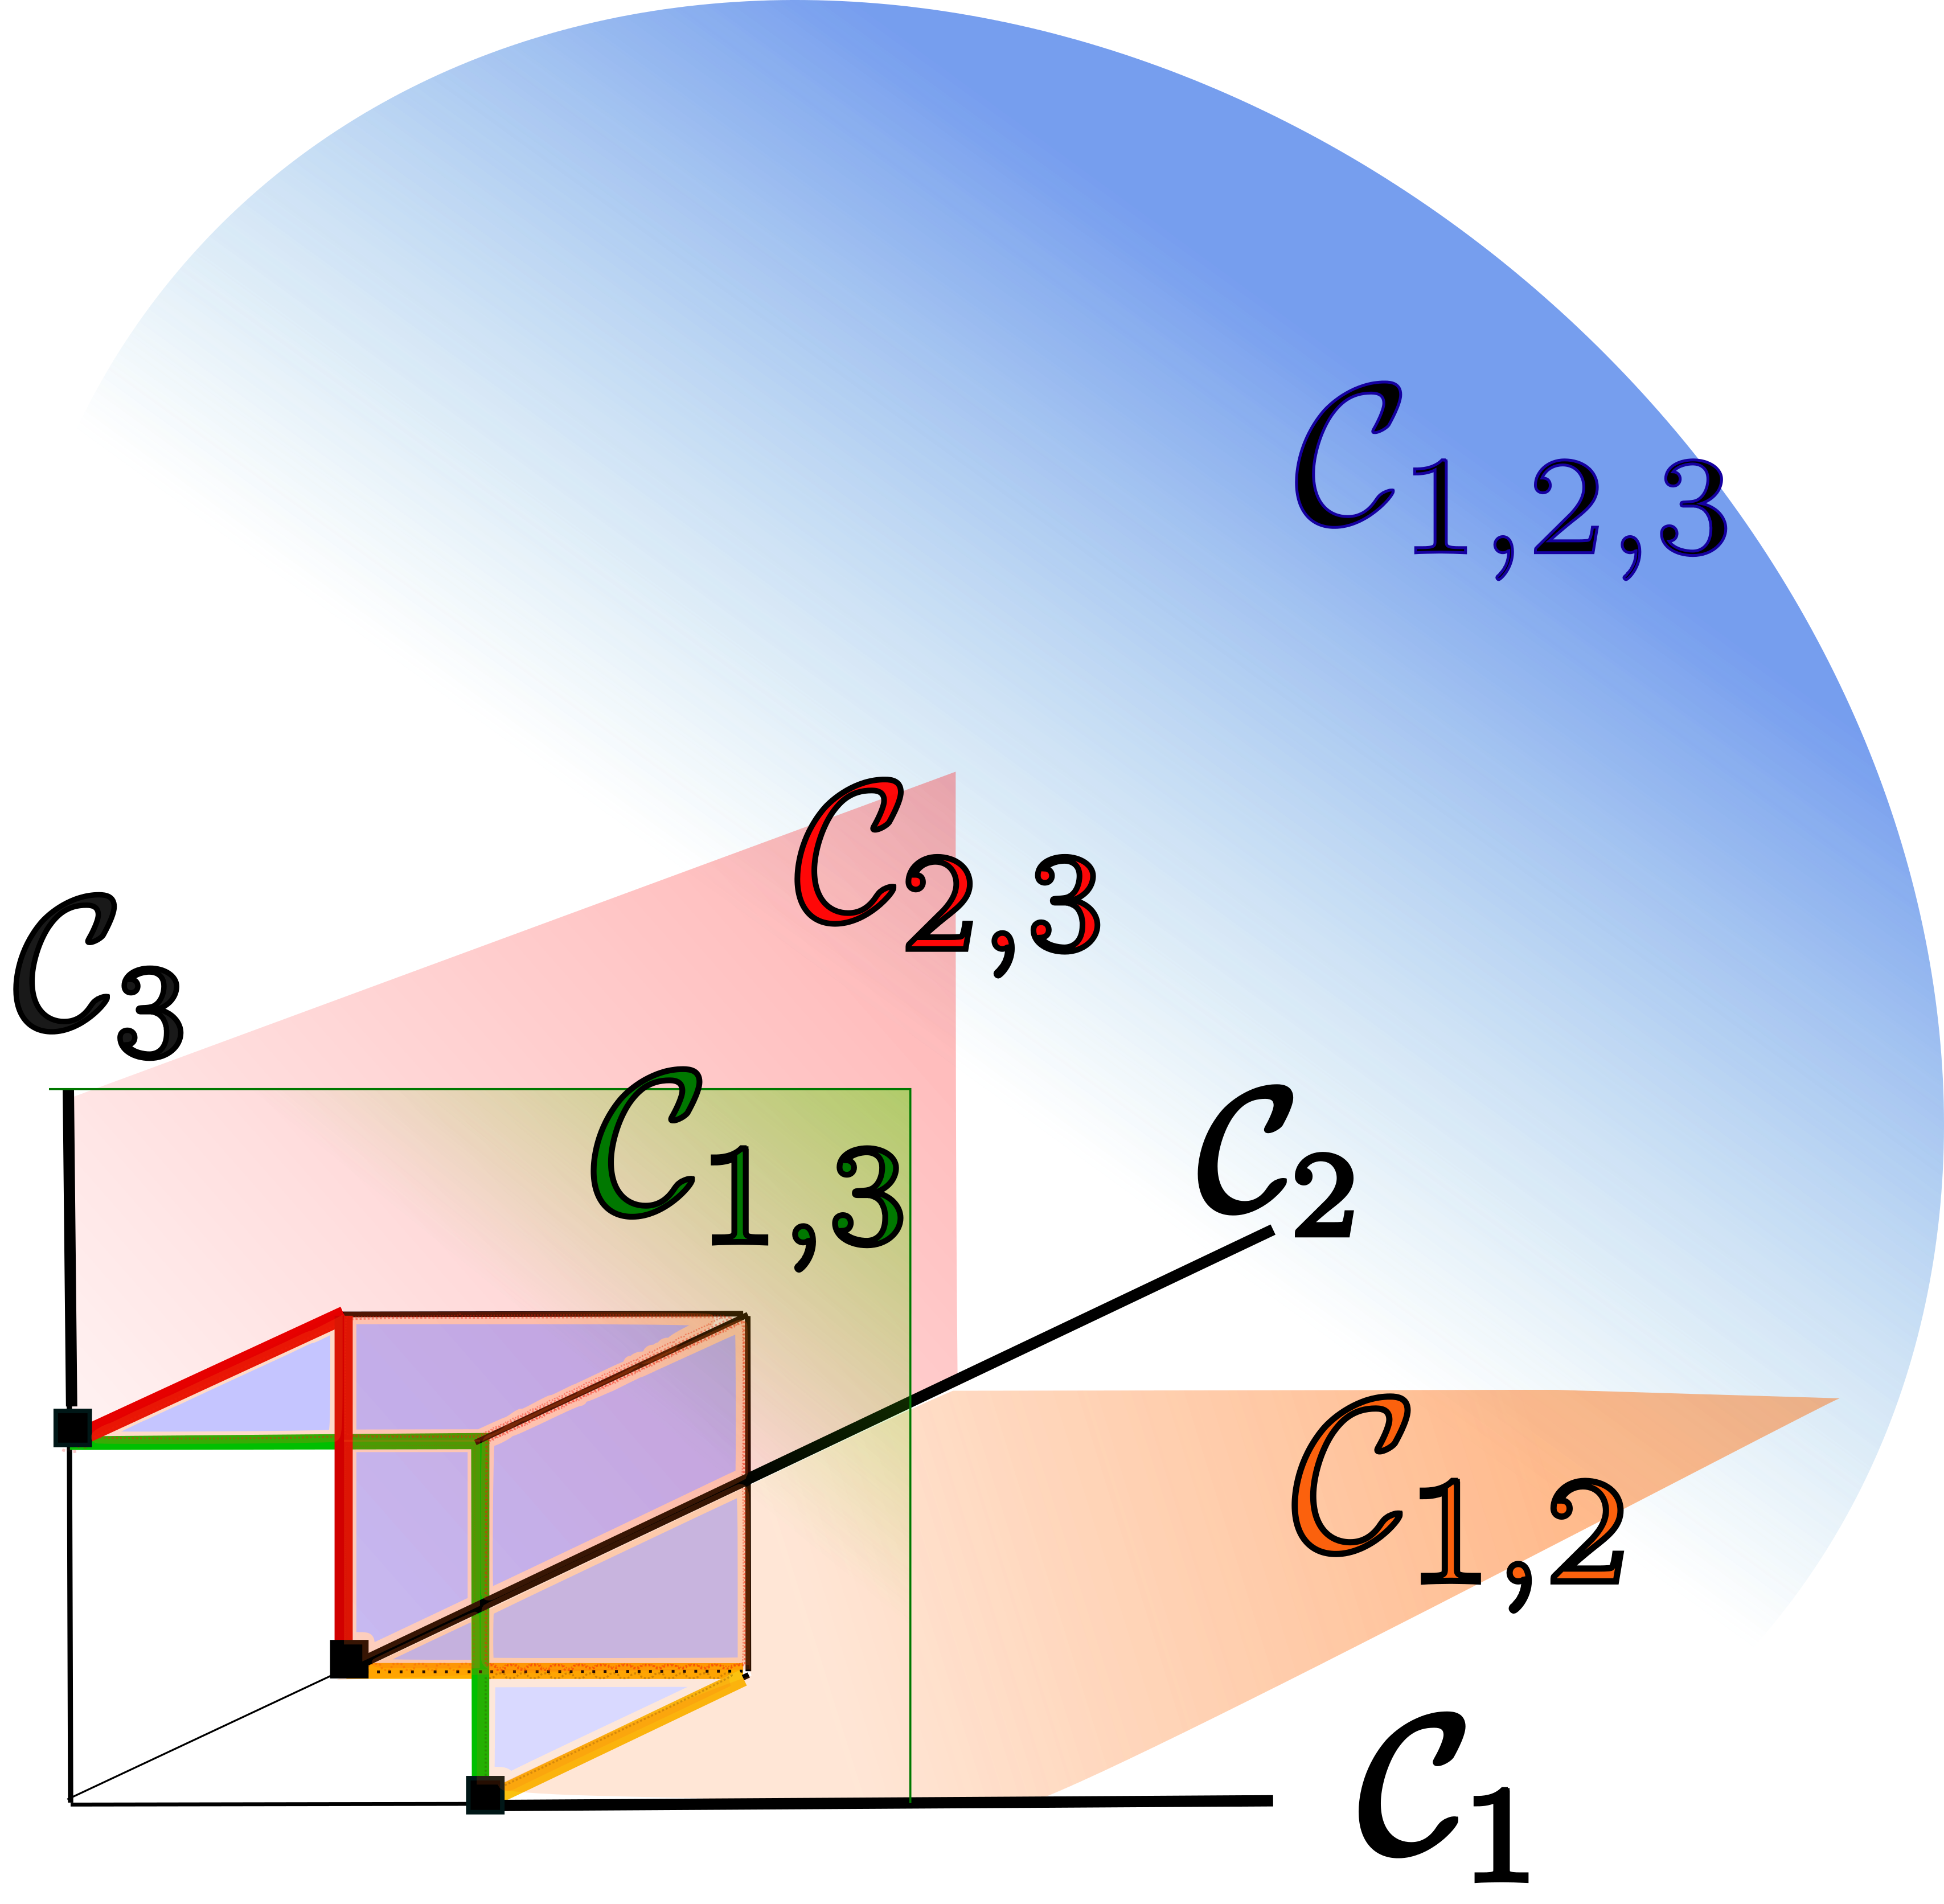
\includegraphics[width=0.4\linewidth]{sourcefigs/cone}
  \end{figure}


  \begin{itemize}
\item How to choose $\epsilon$ in practice?
\item Refine our representation?
\item An alternative notion of sparsity?
  \end{itemize}
\end{frame}






\begin{frame}
\frametitle{Some references:}
\begin{itemize}
\footnotesize{
\item Agarwal 2006, Detecting anomalies in cross-classified streams: a bayesian approach.

\item Aggarwal and Yu 2001, Outlier detection for high dimensional data.


\item Chandola, Banerjee, and Kumar 2009, Anomaly detection: A survey.

%\item A. L. M. Dekkers, J. H. J. Einmahl, and L. De Haan. A moment estimator for the index of an extreme-value distribution, 1989

\item Clifton, Hugueny and Tarassenko 2011, Novelty detection with multivariate extreme value statistics.

\item Désir, Bernard, Petitjean and Heutte 2012, A New Random Forest Method for One-Class Classification.

\item Einmahl and Mason 1992, Generalized quantile processes.

% \item Einmahl and Segers 2009 Maximum empirical likelihood estimation of the spectral measure of an extreme-value distribution

\item Einmahl, Krajina and Segers 2012, An m-estimator for tail dependence in arbitrary dimensions.

\item Eskin 2000,  Anomaly detection over noisy data using learned probability distributions.

\item Goix, Sabourin and Clémençon 2015, Learning the dependence structure of rare events: a non-asymptotic study.

\item Goix, Sabourin and Clémençon 2016, Sparse Representation of Multivariate Extremes with Applications to Anomaly Ranking.

\item Goix, Sabourin and Clémençon 2015, On Anomaly Ranking and Excess-Mass Curves.

\item Goix 2016, How to Evaluate the Quality of Unsupervised Anomaly Detection Algorithms?

\item Goix, Brault, Drougard and Chiapino 2016, One Class Splitting Criteria for Random Forests with Application to Anomaly Detection.

\item Hautamaki, Karkkainen and Franti 2004. Outlier detection using k-nearest neighbour graph.

\item de Haan and Ferreira, Extreme value theory, 2006.

\item Hawkins 1980, Identification of outliers.

\item Lee and Roberts 2008, On-line novelty detection using the Kalman filter and extreme value theory.

}
\end{itemize}
\end{frame}



\begin{frame}
\frametitle{Some references:}
\begin{itemize}
\footnotesize{

\item Liu, Ting, Zhou 2008, Isolation forest.

\item Liu and Weng 1991,  Detection of outlying data in bioavailability/bioequivalence studies. 

\item Papadimitriou, Kitagawa, Gibbons and Faloutsos 2002, Loci: Fast outlier detection using the local correlation integral.

\item Polonik 1995, Measuring mass concentrations and estimating density contour cluster-an excess mass approach.

\item Polonik 1997, Minimum volume sets and generalized quantile processes.

\item Qi 1997, Almost sure convergence of the stable tail empirical dependence function in multivariate extreme statistics.

\item Resnick 1987, Extreme Values, Regular Variation, Point Processes.

\item Roberts 1999, Novelty detection using extreme value statistics.

\item Sch{\"o}lkopf, Platt, Shawe-Taylor, Smola, and Williamson 2001, Estimating the support of a high-dimensional distribution.

\item Scott and Nowak 2006, Learning minimum volume sets.

\item J. Segers 2012, Max-stable models for multivariate extremes.

\item Shi and Horvath 2012, Unsupervised learning with random forest predictors.

\item Shyu, Chen, Sarinnapakorn and Chang 2003, A novel anomaly detection scheme based on principal component classifier

\item Tang, Chen, Fu, and W.Cheung 2002. Enhancing effectiveness of outlier detections for low density patterns.

\item Thomas, Feuillard and Gramford 2015, Calibration of One-Class SVM for MV set estimation.

\item Thomas, Clémençon, Feuillard and Gramford 2016, Learning Hyperparameters for Unsupervised Anomaly Detection.

\item Vert and Vert 2006, Consistency and Convergence Rates of One-Class SVMs and Related Algorithms
}
\end{itemize}
\end{frame}


\begin{frame}
\frametitle{Damex algorithm}
\begin{center}

% \begin{minipage}{0.95\linewidth}
\begin{block}{DAMEX in $O(dn\log n)$}

\begin{algorithmic} 
\STATE {\bf Input:} parameters $\epsilon>0$,~~ $k = k(n)$\\~\\ %$\Phi_{\min}\geq 0$.
  \FOR{$i=1,\ldots,n$}
\STATE {\green $\#$ Standardize \emph{via} marginal rank-transformation:}
\STATE $\hat V_i := \big (1/(1- \hat F_j (X_i^j))\big)_{j=1,\ldots,d}$~. 

\IF{$\hat V_i > \frac{n}{k}$}
\STATE {\green $\#$ Assign to each $\hat V_i$ the cone  $\frac{n}{k}\mathcal{C}_\alpha^\epsilon$  it belongs to:}
\STATE $\alpha = \alpha(V_i)$  \\
\STATE $c_\alpha$ ++
\ENDIF
  \ENDFOR
\STATE $\Phi_n^{\alpha,\epsilon} := \frac{n}{k} c_\alpha $ \\~\\
\STATE {\bf Output:} (sparse) representation of the dependence
  structure:
$\Phi_n^{\alpha,\epsilon} = \widehat{\Phi}(\Omega_\alpha) = \frac{n}{k}\mathbb{P}_n( \hat V \in \frac{n}{k}\mathcal{C}_\alpha^\epsilon)$, estimate of the $\alpha$-mass of $\Phi$ for every $\alpha$.

 %$(\mu_n^{\alpha,\epsilon})_{\alpha\subset\{1,\ldots, d\}, \mu_n^{\alpha,\epsilon}>\mu_{\min}}$.

\begin{align*}
\widehat{\mathcal{M}} := (\Phi_n^{\alpha,\epsilon})_{\alpha\subset\{1,\ldots, d\}, \Phi_n^{\alpha,\epsilon}>\Phi_{\min}}
\end{align*}

\end{algorithmic}
% \end{minipage}

\end{block}
\end{center}

\end{frame}



% \begin{frame}
% \frametitle{Damex benchmark}
% \begin{figure}[H]
%   \centering
%   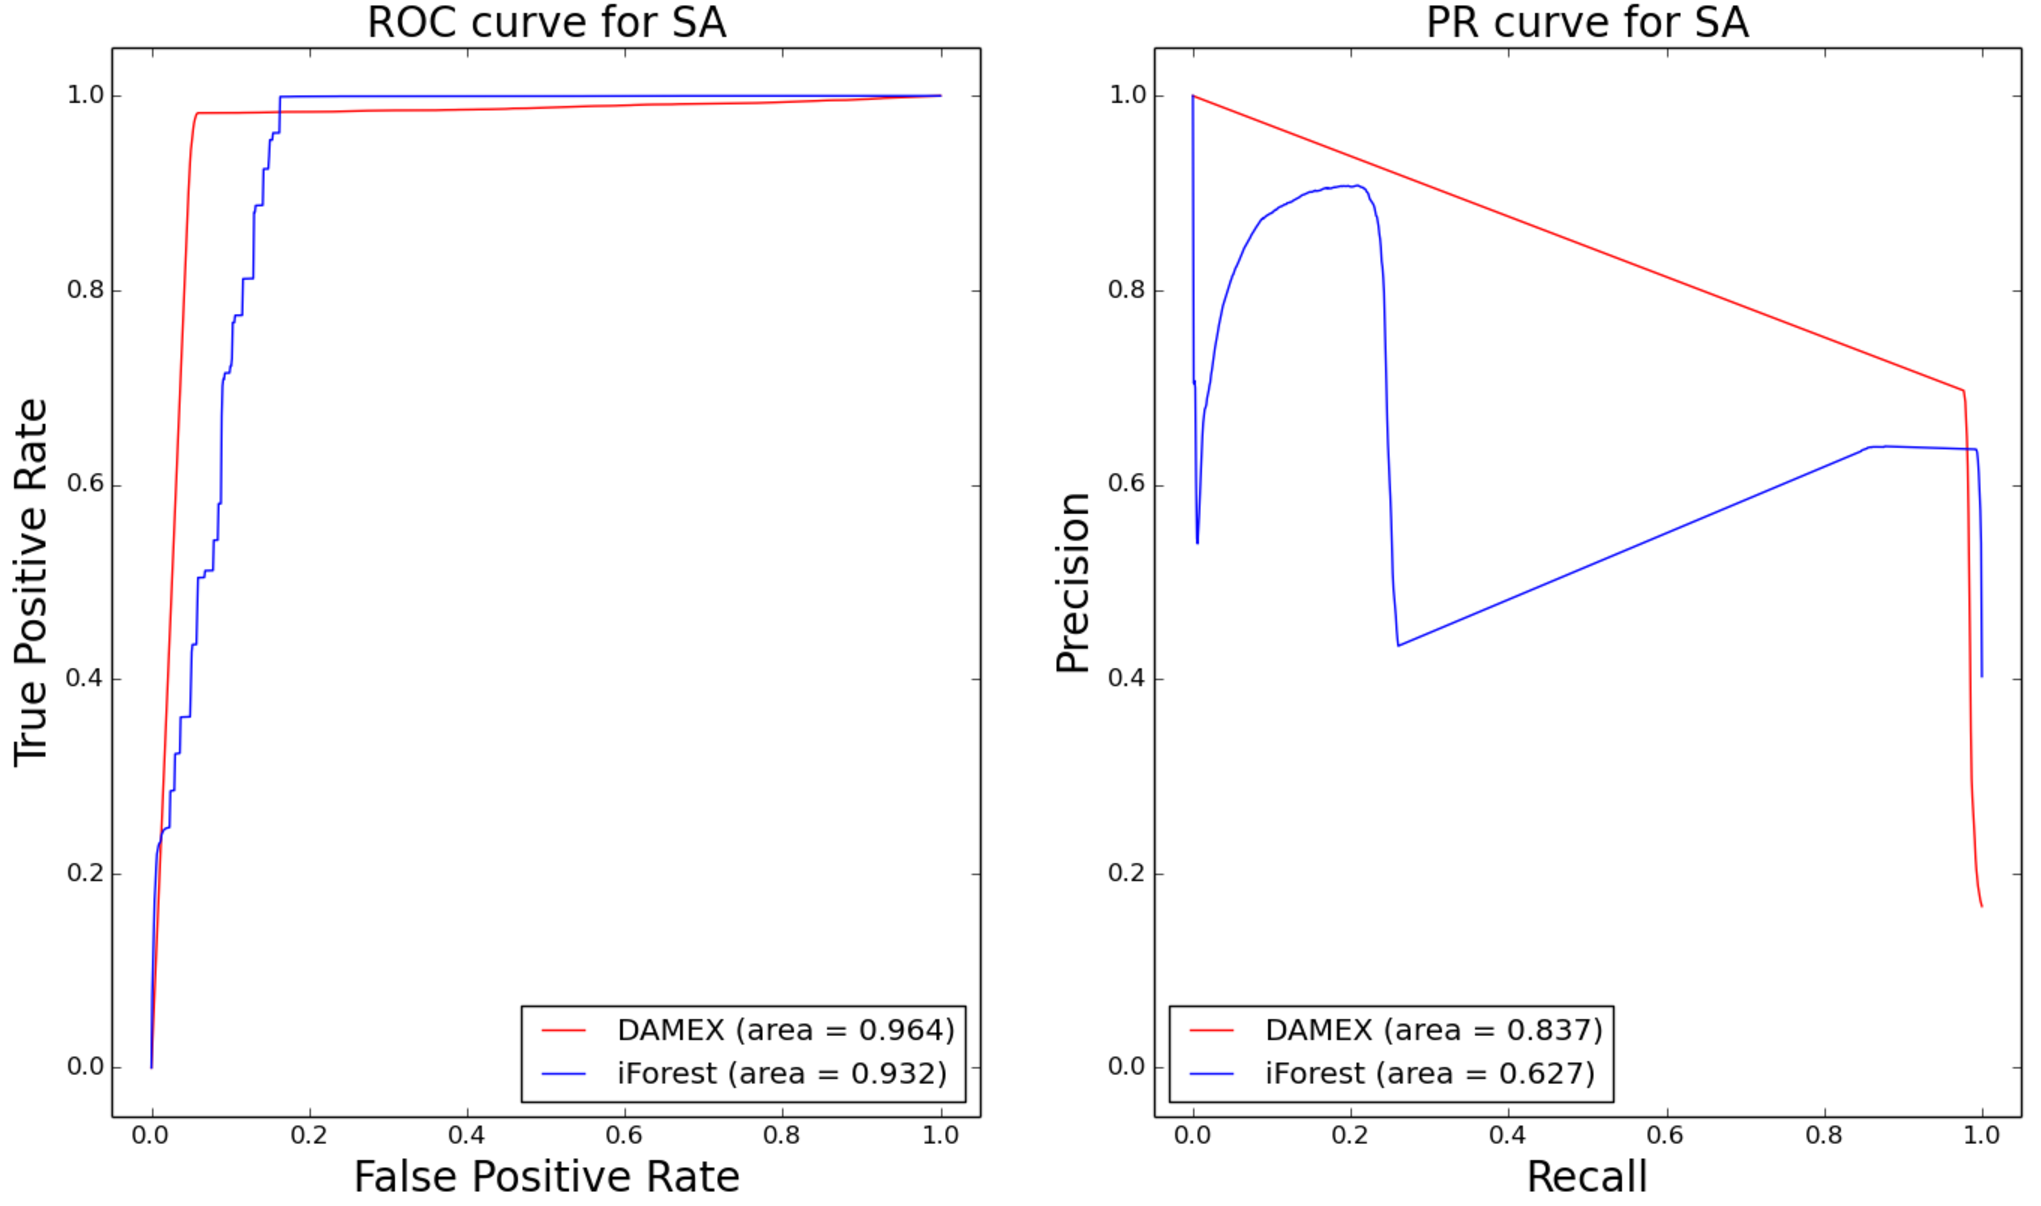
\includegraphics[width = 1. \textwidth]{SA-lb-semi-supervised-average-0001.pdf}
%   \caption{ROC and PR curve on SA dataset}
%   \label{SA}
% \end{figure}
% \end{frame}




% \begin{frame}
% \frametitle{Damex benchmark}
% \begin{table}[h]
% \centering
% \begin{tabular}{lcc}
%   \toprule
%   ~           & number of samples  & number of features \\
%   \midrule
%   shuttle     & 85849              & 9                  \\
%   forestcover & 286048             & 54                 \\
%   SA          & 976158             & 41                 \\
%   SF          & 699691             & 4                  \\
%   http        & 619052             & 3                  \\
%   % smtp        & 95373              & 3                  \\
%   \bottomrule
% \end{tabular}
% \caption{Datasets characteristics}
% \label{table:data}


% % \begin{tabular}{lcccc}
% %   \toprule
% % Dataset      &\multicolumn{2}{c}{iForest}& \multicolumn{2}{c}{DAMEX}\\
% % \midrule
% % ~            &AUC ROC       & AUC PR     &AUC ROC     &AUC PR       \\
% % shuttle      & 0.957        & 0.987      &$\mb{0.988}$&$\mb{0.996}$ \\
% % forestcover  & 0.667        & 0.201      &$\mb{0.976}$&$\mb{0.805}$ \\
% % http         & 0.561        & 0.321      &$\mb{0.981}$&$\mb{0.742}$ \\
% % %smtp         & $\mb{0.900}$ &$\mb{0.004}$&0.898       &0.003        \\
% % SF           & 0.134        & 0.189      &$\mb{0.988}$&$\mb{0.973}$ \\
% % SA           & 0.932        &0.625       &$\mb{0.945}$&$\mb{0.818}$ \\ 
% % \bottomrule
% % \end{tabular}
% % \caption{Results on extreme regions with standard parameters $(k,\epsilon) = (n^{1/2}, 0.01)$}
% \end{table}
% \end{frame}


% \begin{frame}
% \frametitle{Damex benchmark}
% \begin{figure}[H]
%   \centering
%   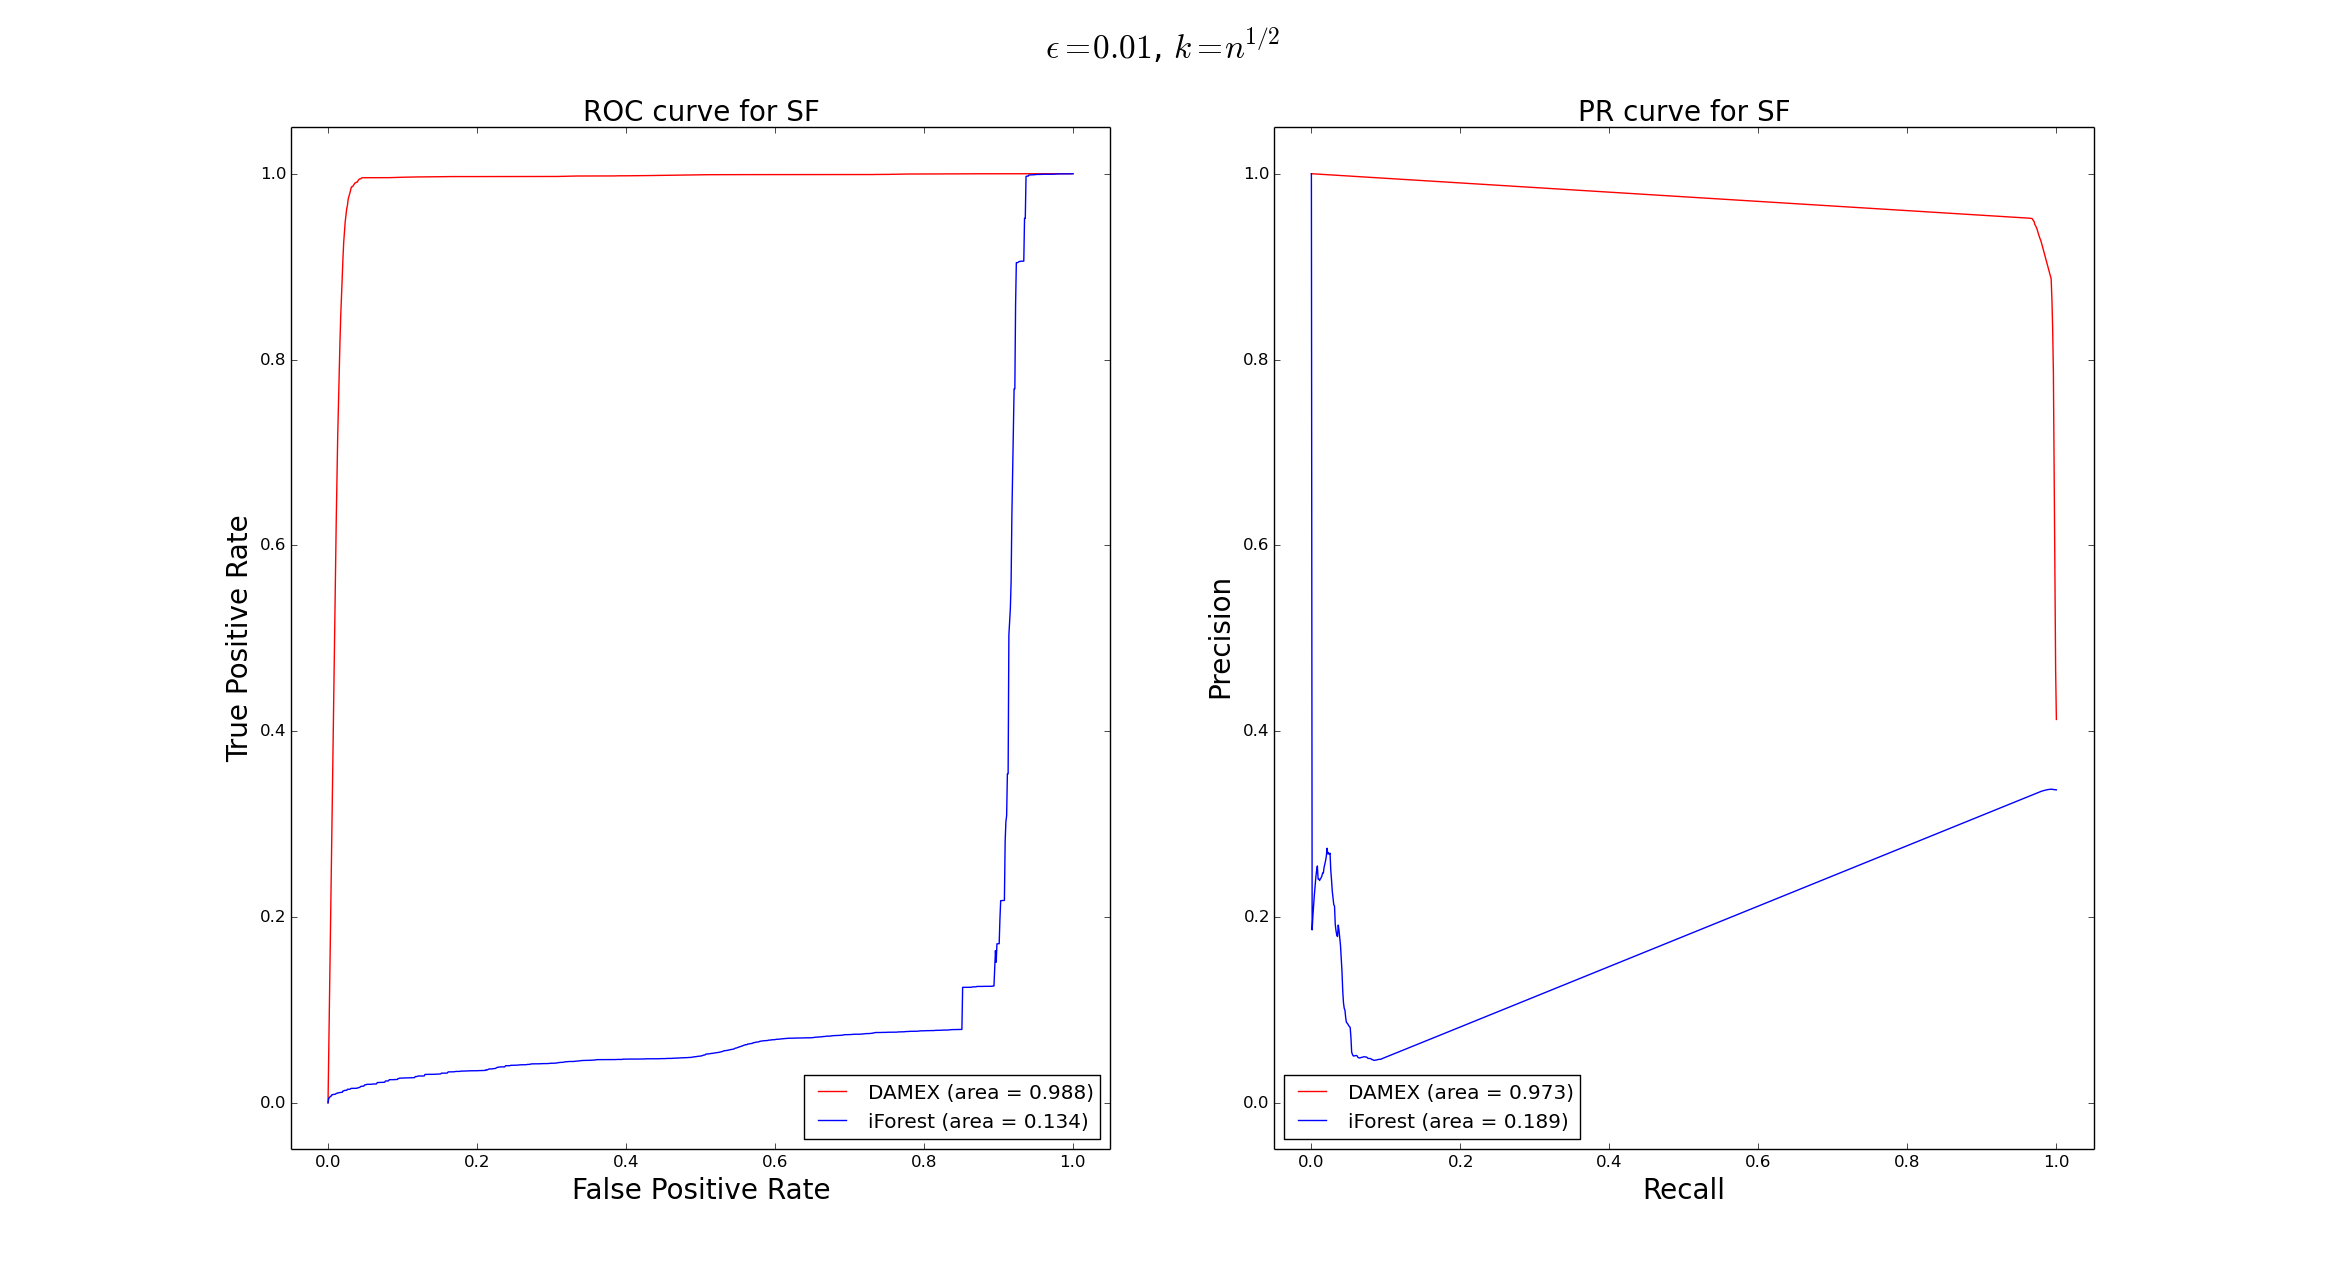
\includegraphics[width = 1. \textwidth]{SF-4d-lb-semi-supervised-average-rect-01}
%   \caption{ROC and PR curve on SF dataset}
%   \label{SF}
% \end{figure}
% \end{frame}



% \begin{frame}
% \frametitle{Damex benchmark}
% \begin{figure}[H]
%   \centering
%   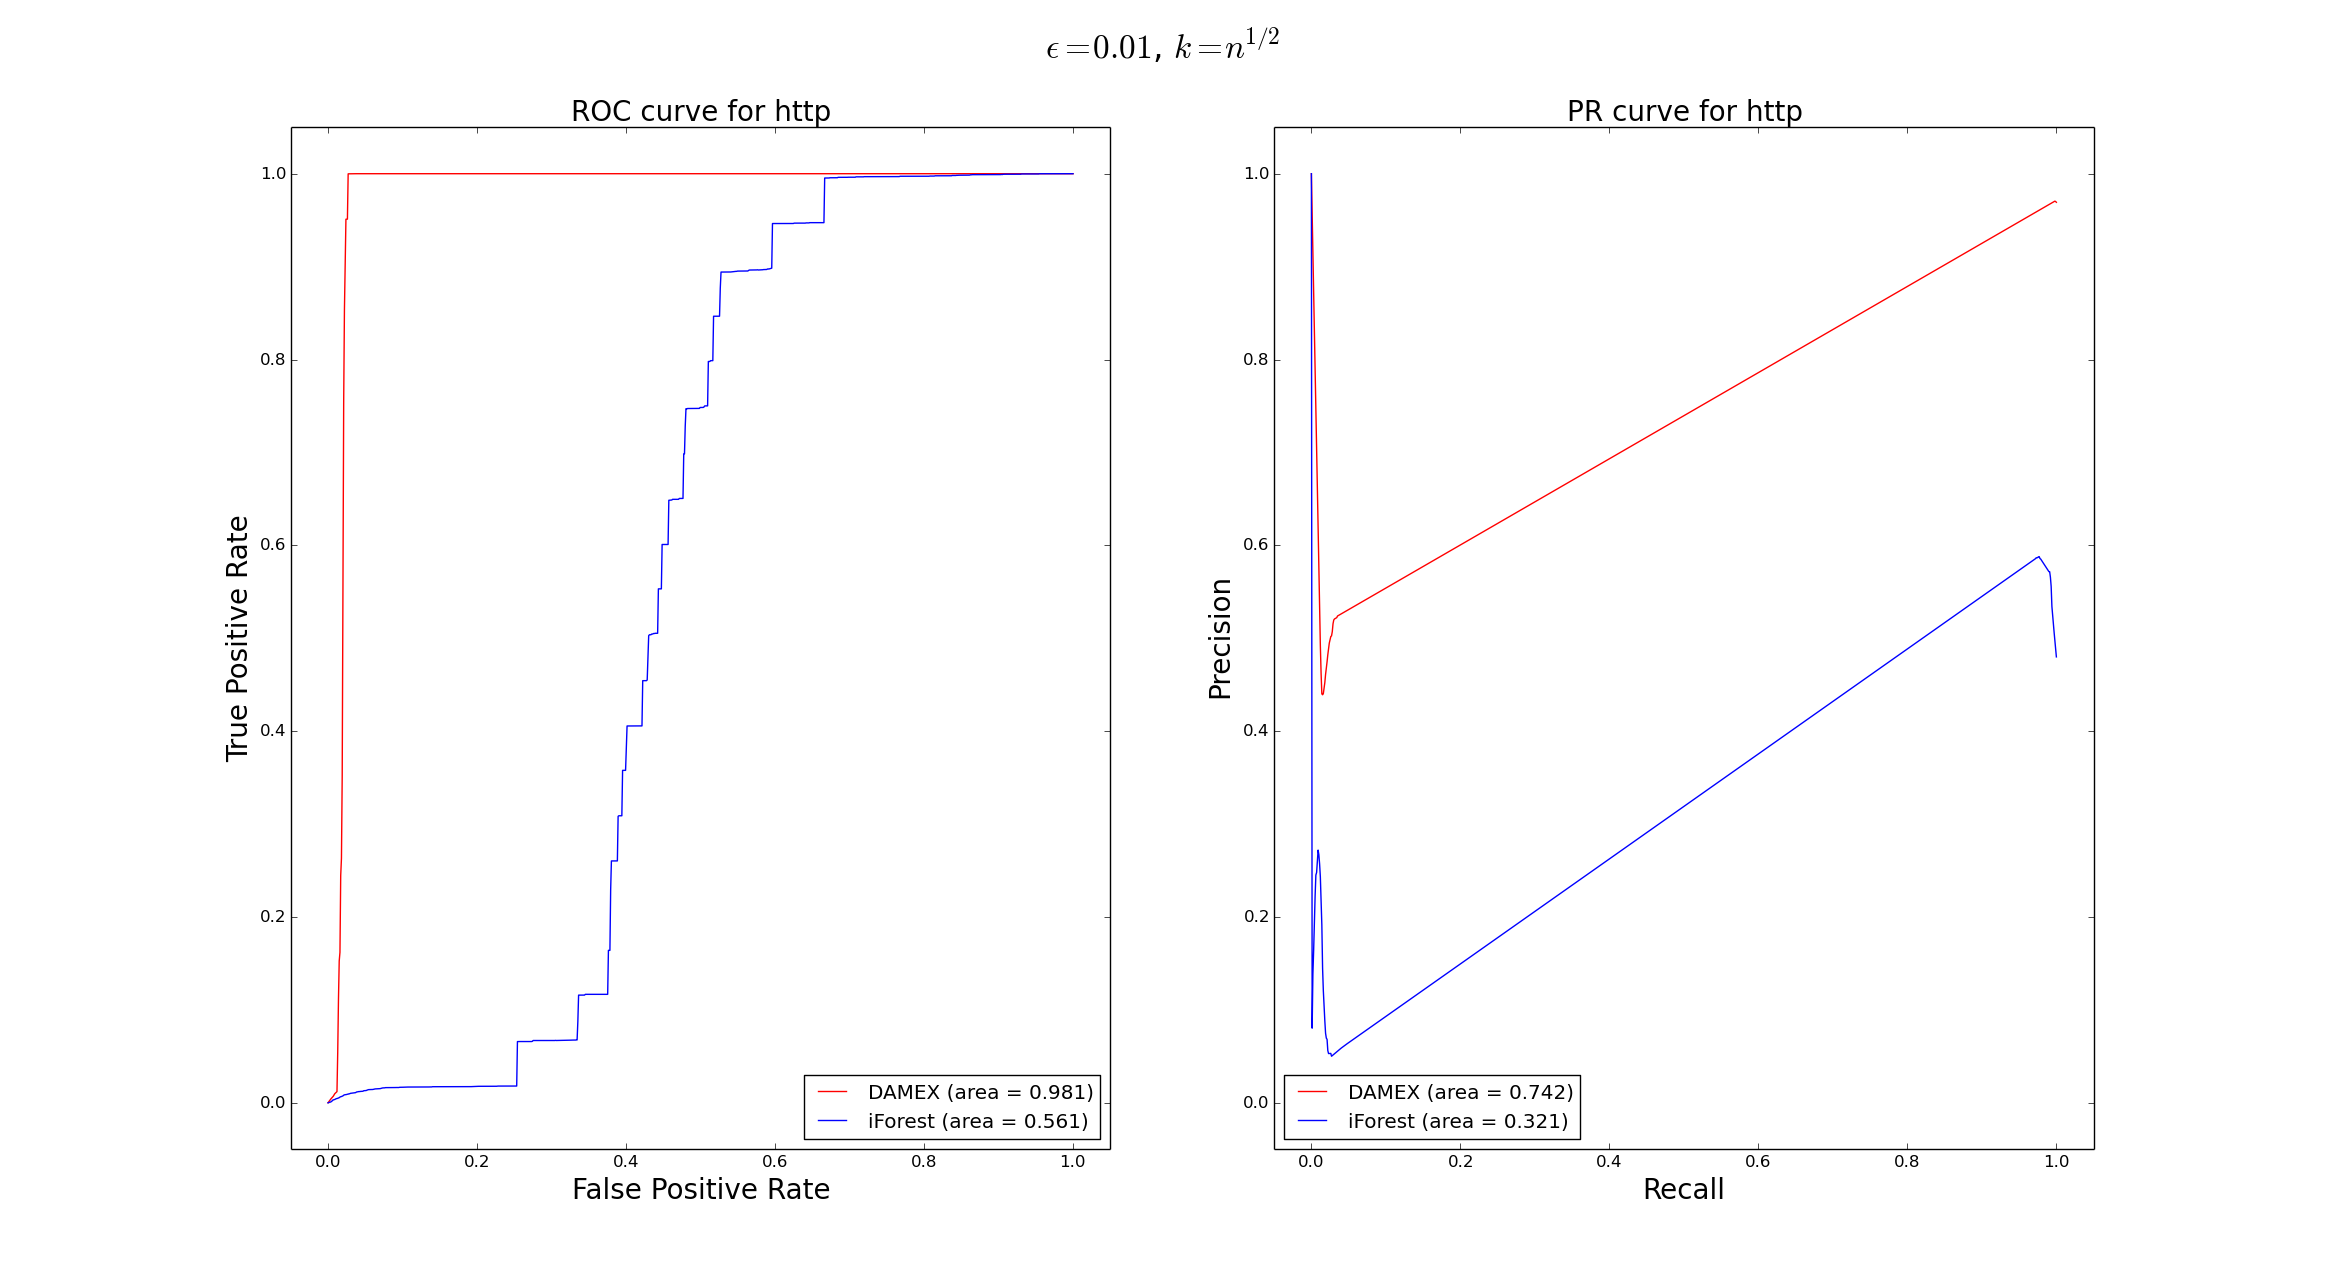
\includegraphics[width = 1. \textwidth]{http-3d-semi-supervised-average-rect-01}
%   \caption{ROC and PR curve on http dataset}
%   \label{http}
% \end{figure}
% \end{frame}


% \begin{frame}
% \frametitle{Damex benchmark}
% \begin{figure}[H]
%   \centering
%   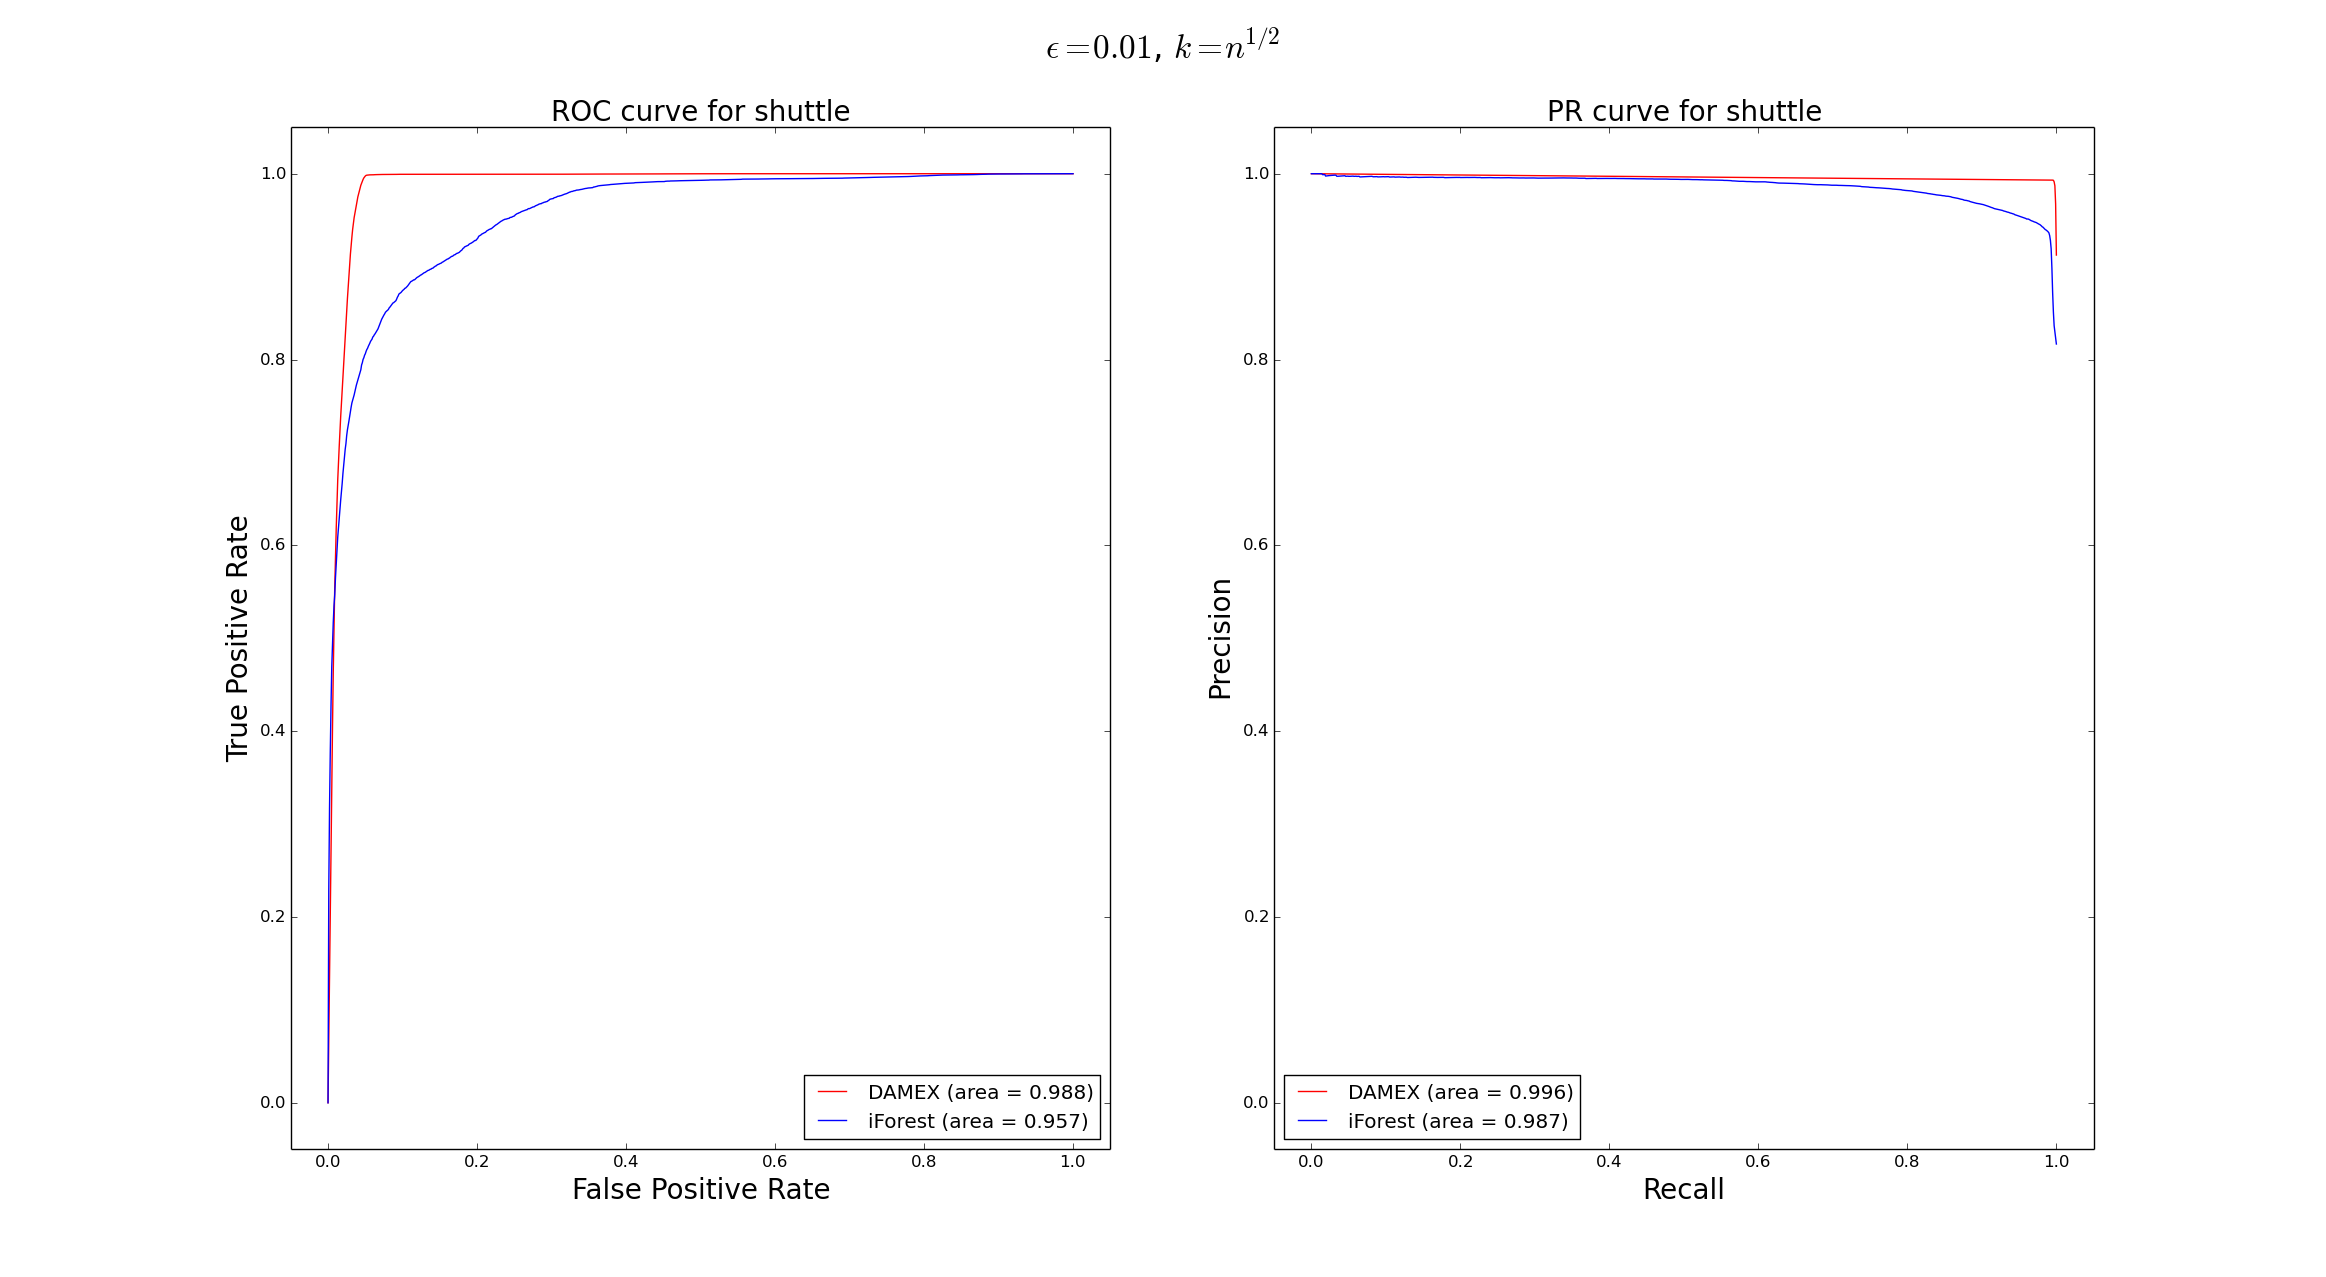
\includegraphics[width = 1. \textwidth]{shuttle-semi-supervised-average-rect-01}
%   \caption{ROC and PR curve on shuttle dataset}
%   \label{shuttle}
% \end{figure}
% \end{frame}

% \begin{frame}
% \frametitle{Damex benchmark}
% \begin{figure}[H]
%   \centering
%   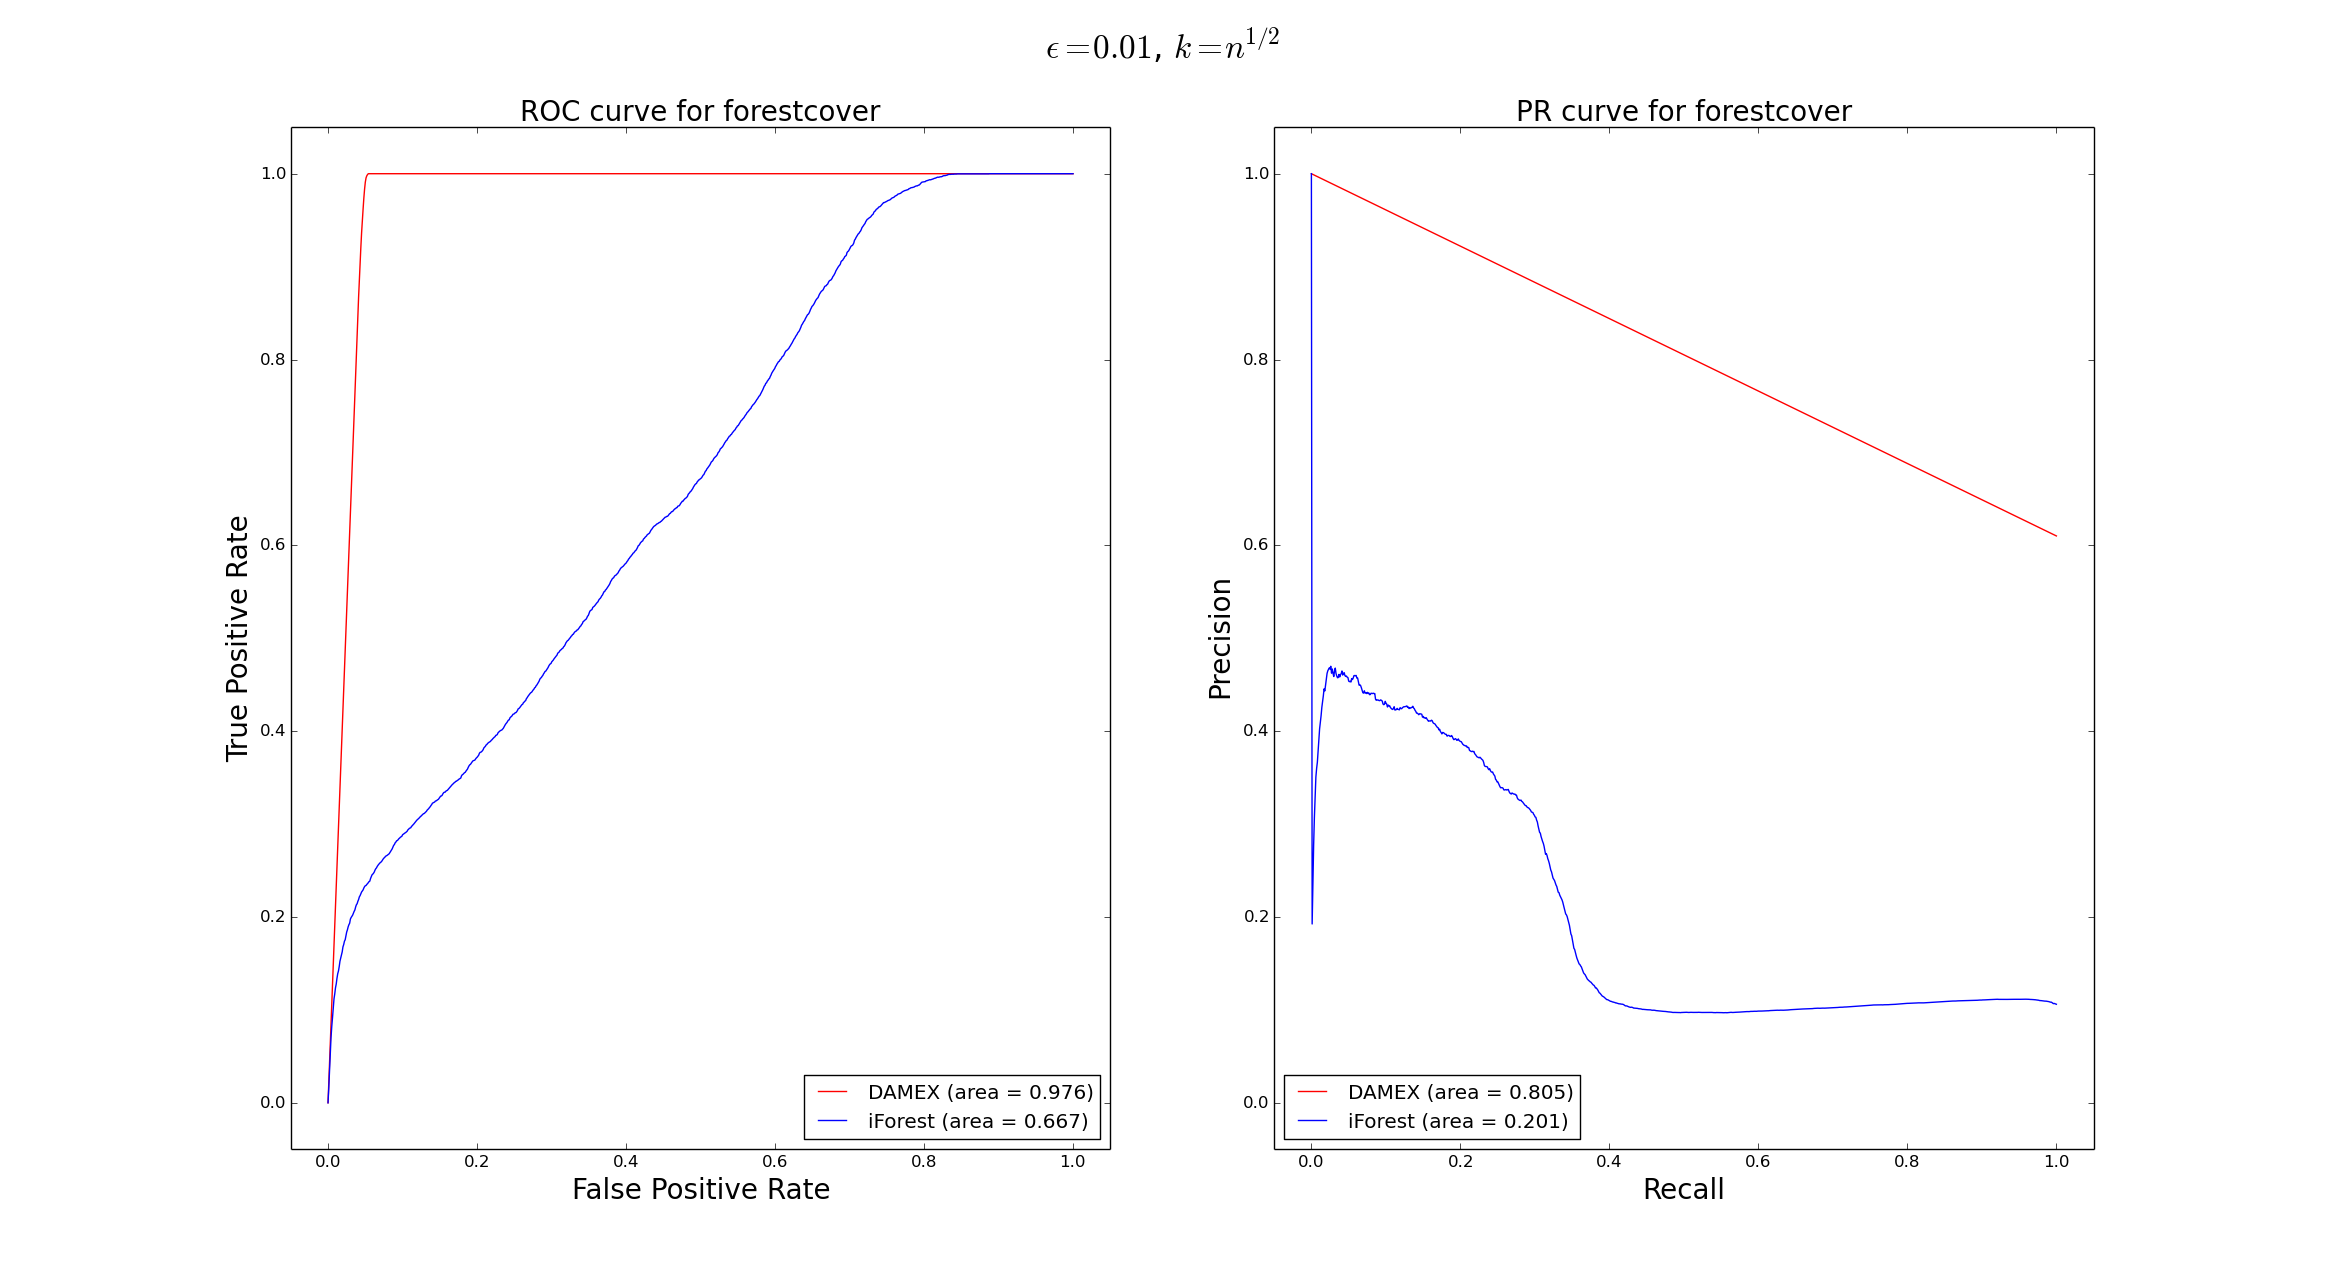
\includegraphics[width = 1. \textwidth]{forestcover-semi-supervised-average-rect-01}
%   \caption{ROC and PR curve on forestcover dataset}
%   \label{forestcover}
% \end{figure}
% \end{frame}





\begin{frame}
\frametitle{EM/MV random projection benchmark}
\begin{block}{Does performance in term of EM/MV correspond to performance in term of ROC/PR?}

\begin{itemize}
\item \textbf{Experiments:}
{\small
12 datasets, 3 AD algorithms (LOF, OCSVM, iForest)
$\to$ 36 possible pairwise comparisons:
\begin{align*}
\bigg\{~~\Big(A_1 \text{~on~} \mathcal{D},~ A_2 \text{~on~} \mathcal{D}\Big),~~ & A_1, A_2 \in \{\text{iForest, LOF, OCSVM}\}, \\
& \mathcal{D} \in \{\text{adult, http, \ldots, spambase}\} ~~\bigg\}.
\end{align*}
}


\item \textbf{Results:}
{ \small
If we only consider the pairs \st~\emph{ROC and PR agree on which algorithm is the best}, we are able (with EM and MV scores) to recover it in $80\%$ of the cases.
}
\end{itemize}


\end{block}
\end{frame}




\begin{frame}{EM/MV random projection benchmark}
\begin{table}[!ht]
\centering
\footnotesize
\caption{\footnotesize Results for the novelty detection setting. One can see that ROC, PR, EM, MV often do agree on which algorithm is the best (in bold), which algorithm is the worse (underlined) on some fixed datasets. When they do not agree, it is often because ROC and PR themselves do not, meaning that the ranking is not clear.}
\tabcolsep=0.11cm
\resizebox{\linewidth}{!} {
\begin{tabular}{l cccc c cccc c cccc}
\toprule
Dataset      & \multicolumn{4}{c}{iForest}& & \multicolumn{4}{c}{OCSVM}&  & \multicolumn{4}{c}{LOF} \\ %& parameters $(\epsilon, k)$\\
  \cmidrule{1-15}

~            & ROC  & PR   & EM    &  MV  &  & ROC  & PR   & EM    & MV     &  & ROC  & PR   & EM    & MV    \\
adult        &\bf 0.661 &\bf 0.277 &\bf 1.0e-04&\bf 7.5e01&  &0.642 &0.206 &2.9e-05& 4.3e02 &  &\underline{0.618} &\underline{0.187}&\underline{1.7e-05}&\underline{9.0e02} \\
http         &0.994 &0.192 &1.3e-03&9.0   &  &\bf 0.999 &\bf 0.970 &\bf 6.0e-03&\bf 2.6  &     &\underline{0.946} &\underline{0.035} &\underline{8.0e-05}&\underline{3.9e02} \\
pima         &0.727 &0.182 &5.0e-07&\bf 1.2e04&  &\bf 0.760 &\bf 0.229 &\bf 5.2e-07&\underline{1.3e04} &   &\underline{0.705} &\underline{0.155} &\underline{3.2e-07}&2.1e04 \\
smtp         &0.907 &\underline{0.005} &\underline{1.8e-04}&\underline{9.4e01}&  &\underline{0.852} &\bf 0.522 &\bf 1.2e-03&8.2    &   &\bf 0.922 &0.189 & 1.1e-03&\bf 5.8    \\
wilt         &0.491 &0.045 &4.7e-05&\underline{2.1e03} & &\underline{0.325} &\underline{0.037} &\bf 5.9e-05&\bf 4.5e02 &   &\bf 0.698 &\bf 0.088 &\underline{2.1e-05}&1.6e03 \\ 
 &&&&&&&&&&&&&& \\
% internet\_ads&0.414 &0.109 &  NA   &  NA    &      &      &       &          &0.540 &0.139 &       &       \\
% SA           &0.988 &0.386 &  NA   &  NA    &      &      &       &          &0.880 &0.018 &       &       \\
% SF           &0.936 &0.038 &  NA   &  NA    &      &      &       &          &0.891 &0.022 &       &       \\
annthyroid   &\bf 0.913 &\bf 0.456 &\bf 2.0e-04&2.6e02 & &\underline{0.699} &\underline{0.237} &\underline{6.3e-05}&\bf 2.2e02 &   &0.823 &0.432 &6.3e-05&\underline{1.5e03} \\
arrhythmia   &\bf 0.763 &\bf 0.487 &\bf 1.6e-04&\bf 9.4e01 & &0.736 &0.449 &1.1e-04&1.0e02   & &\underline{0.730} &\underline{0.413} &\underline{8.3e-05}&\underline{1.6e02} \\
forestcov.   &\underline{0.863} &\underline{0.046} &\underline{3.9e-05}&\underline{2.0e02}&  &0.958 &0.110 &5.2e-05&1.2e02  &  &\bf 0.990 &\bf 0.792 &\bf 3.5e-04&\bf 3.9e01 \\
ionosphere   &\underline{0.902} &\underline{0.529} &\underline{9.6e-05}&\underline{7.5e01} & &\bf 0.977 &\bf 0.898 &\bf 1.3e-04&\bf 5.4e01  &  &0.971 &0.895 &1.0e-04&7.0e01 \\
pendigits    &0.811 &0.197 &2.8e-04&2.6e01 & &\underline{0.606} &\underline{0.112} &\underline{2.7e-04}&\underline{2.7e01}   & &\bf 0.983 &\bf 0.829 &\bf 4.6e-04&\bf 1.7e01 \\
shuttle      &0.996 &0.973 &1.8e-05&5.7e03 & &\underline{0.992} &\underline{0.924} &\bf 3.2e-05&\bf 2.0e01   & &\bf 0.999 &\bf 0.994 &\underline{7.9e-06}&\underline{2.0e06} \\
spambase     &\bf 0.824 &\bf 0.371 &\bf 9.5e-04&\bf 4.5e01&  &\underline{0.729} &0.230 &4.9e-04&1.1e03  &  &0.754 &\underline{0.173} &\underline{2.2e-04}&\underline{4.1e04} \\
\bottomrule
\end{tabular}
}
\end{table}

\end{frame}



\begin{frame}
\frametitle{OCRF Benchmark}
\begin{table}[ht]
\caption{ Results for the novelty detection setting %(novelty detection framework).
%We compare various methods from the state-of-the-art (top line) to OneClassRF over different classical datasets (leftmost column).
}
\label{ocrf:table:results-semisupervised}
\centering
%\scriptsize
\tabcolsep=0.1cm
\resizebox{1.\linewidth}{!} {
\begin{tabular}{ l  c@{\extracolsep{0.1cm}}c c@{\extracolsep{0.1cm}}c c@{\extracolsep{0.1cm}}c c@{\extracolsep{0.1cm}}c c@{\extracolsep{0.1cm}}c c@{\extracolsep{0.1cm}}c c@{\extracolsep{0.1cm}}c c@{\extracolsep{0.1cm}}c }
\toprule
%
Datasets & \multicolumn{2}{c }{OneClassRF} & \multicolumn{2}{c }{iForest} & \multicolumn{2}{c }{OCRF\small{sampl.}} & \multicolumn{2}{c }{OCSVM}& \multicolumn{2}{c }{LOF}& \multicolumn{2}{c }{Orca}& \multicolumn{2}{c }{LSAD}& \multicolumn{2}{c }{RFC}  \\%& parameters $(\epsilon, k)$\\
  \cmidrule{1-17}
~     & ROC &  PR & ROC &  PR & ROC & PR  & ROC & PR  & ROC & PR  &ROC  & PR  & ROC &  PR & ROC & PR  \\
adult        &        \textbf{0.665} & \textbf{0.278} & 0.661 & 0.227 & NA & NA & 0.638 & 0.201 & 0.615 & 0.188 & 0.606 & 0.218 &  0.647    & 0.258     & NA & NA \\
annthyroid   &        \textbf{0.936} & 0.468 & 0.913 & 0.456 & 0.918 & \textbf{0.532} & 0.706 & 0.242 & 0.832 & 0.446 & 0.587 & 0.181 &  0.810    & 0.327     & NA & NA \\
arrhythmia   &        0.684 & 0.510 & 0.763 & 0.492 & 0.639 & 0.249 & \textbf{0.922} & \textbf{0.639} & 0.761 & 0.473 & 0.720 & 0.466 &  0.778    & 0.514     & 0.716 & 0.299 \\
forestcover  &        0.968 & 0.457 & 0.863 & 0.046 & NA & NA & NA & NA & \textbf{0.990} & \textbf{0.795} & 0.946 & 0.558 &  0.952    & 0.166     & NA & NA \\
http         &        \textbf{0.999} & \textbf{0.838} & 0.994 & 0.197 & NA & NA & NA & NA & NA & NA & \textbf{0.999} & 0.812 &  0.981    & 0.537     & NA & NA \\
ionosphere   &        0.909 & 0.643 & 0.902 & 0.535 & 0.859 & 0.609 & 0.973 & 0.849 & 0.959 & 0.807 & 0.928 & \textbf{0.910} &  \textbf{0.978}    & 0.893     & 0.950 & 0.754 \\
pendigits    &        0.960 & 0.559 & 0.810 & 0.197 & 0.968 & 0.694 & 0.603 & 0.110 & 0.983 & 0.827 & \textbf{0.993} & \textbf{0.925} &  0.983    & 0.752     & NA & NA \\
pima         &        0.719 & 0.247 & 0.726 & 0.183 & \textbf{0.759} & \textbf{0.266} & 0.716 & 0.237 & 0.700 & 0.152 & 0.588 & 0.175 &  0.713    & 0.216     & 0.506 & 0.090 \\
shuttle      &        \textbf{0.999} & \textbf{0.998} & 0.996 & 0.973 & NA & NA & 0.992 & 0.924 & \textbf{0.999} & 0.995 & 0.890 & 0.782 &  0.996    & 0.956     & NA & NA \\
smtp         &        0.922 & 0.499 & 0.907 & 0.005 & NA & NA & 0.881 & \textbf{0.656} & \textbf{0.924} & 0.149 & 0.782 & 0.142 &  0.877    & 0.381     & NA & NA \\
spambase     &        \textbf{0.850} & 0.373 & 0.824 & 0.372 & 0.797 & \textbf{0.485} & 0.737 & 0.208 & 0.746 & 0.160 & 0.631 & 0.252 &  0.806    & 0.330     & 0.723 & 0.151 \\
wilt         &        0.593 & 0.070 & 0.491 & 0.045 & 0.442 & 0.038 & 0.323 & 0.036 & 0.697 & 0.092 & 0.441 & 0.030 &  0.677    & 0.074     & \textbf{0.896} & \textbf{0.631} \\
%internet_ads &     &       & & & & & & & &\\
\cmidrule{1-17}
average:    & \textbf{0.850} & \textbf{0.495} & 0.821 & 0.311 & 0.769 & 0.410 & 0.749 & 0.410 & 0.837 & 0.462 & 0.759 & 0.454 & \textbf{0.850}  & 0.450 &  0.758  & 0.385 \\
cum. train time: & \multicolumn{2}{c }{\textbf{61s}} & \multicolumn{2}{c }{68s} & \multicolumn{2}{c }{NA} & \multicolumn{2}{c }{NA}& \multicolumn{2}{c }{NA}& \multicolumn{2}{c }{2232s}& \multicolumn{2}{c }{73s}& \multicolumn{2}{c }{NA}  \\

  \bottomrule
\end{tabular}
}
\end{table}

\end{frame}



\begin{frame}
\frametitle{Datasets}

\begin{table}[ht]
% \caption{Original datasets characteristics}
% \label{ocrf:table:data}
\centering
\footnotesize
%\tabcolsep=0.08cm
\resizebox{\linewidth}{!} {
\begin{tabular}{lccll}
  \toprule
  Datasets        & nb of samples      & nb of features     & ~~~~~~~~~~~~~~~~~~~~~~~~~anomaly class      & ~                  \\ \midrule
  adult       & 48842              & 6                  &    class '$>50K$'                           &      (23.9\%)      \\
  annthyroid  & 7200               & 6                  &    classes $\neq$ 3                         &        (7.42\%)    \\
  arrhythmia  & 452                & 164                &    classes $\neq$ 1 (features 10-14 removed)&  (45.8\%)          \\
  forestcover & 286048             & 10                 &    class 4  (vs. class 2 )                  &           (0.96\%) \\
  http        & 567498             & 3                  &      attack                                 &    (0.39\%)        \\
  ionosphere  & 351                & 32                 &    bad                                      &       (35.9\%)     \\
  pendigits   & 10992              & 16                 &    class 4                                  &        (10.4\%)    \\
  pima        & 768                & 8                  &    pos (class 1)                            &        (34.9\%)    \\
  shuttle     & 85849              & 9                  &      classes $\neq$ 1 (class 4 removed)     &  (7.17\%)          \\
  smtp        & 95156              & 3                  &      attack                                 &    (0.03\%)        \\
  spambase    & 4601               & 57                 &    spam                                     &           (39.4\%) \\
  wilt        & 4839               & 5                  &    class 'w' (diseased trees)               &    (5.39\%)        \\
  \bottomrule
\end{tabular}
}
\end{table}


\end{frame}

\end{document}
